%% abtex2-modelo-trabalho-academico.tex, v-1.9.2 laurocesar
%% Copyright 2012-2014 by abnTeX2 group at http://abntex2.googlecode.com/ 
%%
%% This work may be distributed and/or modified under the
%% conditions of the LaTeX Project Public License, either version 1.3
%% of this license or (at your option) any later version.
%% The latest version of this license is in
%%   http://www.latex-project.org/lppl.txt
%% and version 1.3 or later is part of all distributions of LaTeX
%% version 2005/12/01 or later.
%%
%% This work has the LPPL maintenance status `maintained'.
%% 
%% The Current Maintainer of this work is the abnTeX2 team, led
%% by Lauro César Araujo. Further information are available on 
%% http://abntex2.googlecode.com/
%%
%% This work consists of the files abntex2-modelo-trabalho-academico.tex,
%% abntex2-modelo-include-comandos and abntex2-modelo-references.bib
%%

% ------------------------------------------------------------------------
% ------------------------------------------------------------------------
% abnTeX2: Modelo de Trabalho Academico (tese de doutorado, dissertacao de
% mestrado e trabalhos monograficos em geral) em conformidade com 
% ABNT NBR 14724:2011: Informacao e documentacao - Trabalhos academicos -
% Apresentacao
% ------------------------------------------------------------------------
% ------------------------------------------------------------------------

%-------------------------------------------------------------------------
% Modelo adaptado especificamente para o contexto do PPgSI-EACH-USP por 
% Marcelo Fantinato, com auxílio dos Professores Norton T. Roman, Helton
% H. Bíscaro e Sarajane M. Peres, em 2015, com muitos agradecimentos aos 
% criadores da classe e do modelo base.
%
% 20/06/2017: inclusão de "lista de quadros" com base no especificado em:
% https://github.com/abntex/abntex2/wiki/HowToCriarNovoAmbienteListing,
% de autoria de "Eduardo de Santana Medeiros Alexandre".
%
%-------------------------------------------------------------------------

\documentclass[
	% -- opções da classe memoir --
	12pt,				% tamanho da fonte
	% openright,			% capítulos começam em pág ímpar (insere página vazia caso preciso)
	oneside,			% para impressão apenas no anverso (apenas frente). Oposto a twoside
	a4paper,			% tamanho do papel. 
	% -- opções da classe abntex2 --
	%chapter=TITLE,		% títulos de capítulos convertidos em letras maiúsculas
	%section=TITLE,		% títulos de seções convertidos em letras maiúsculas
	%subsection=TITLE,	% títulos de subseções convertidos em letras maiúsculas
	%subsubsection=TITLE,% títulos de subsubseções convertidos em letras maiúsculas
	% -- opções do pacote babel --
	english,			% idioma adicional para hifenização
	%french,				% idioma adicional para hifenização
	%spanish,			% idioma adicional para hifenização
	brazil				% o último idioma é o principal do documento
	]{abntex2ppgsi}

% ---
% Pacotes básicos 
% ---
% \usepackage{lmodern}			% Usa a fonte Latin Modern			
% \usepackage[T1]{fontenc}		% Selecao de codigos de fonte.
\usepackage[utf8]{inputenc}		% Codificacao do documento (conversão automática dos acentos)
\usepackage{lastpage}			% Usado pela Ficha catalográfica
\usepackage{indentfirst}		% Indenta o primeiro parágrafo de cada seção.
\usepackage{color}				% Controle das cores
\usepackage{graphicx}			% Inclusão de gráficos
\usepackage{microtype} 			% para melhorias de justificação
\usepackage{pdfpages}     %para incluir pdf
\usepackage{algorithm}			%para ilustrações do tipo algoritmo
\usepackage{mdwlist}			%para itens com espaço padrão da abnt
\usepackage[noend]{algpseudocode}			%para ilustrações do tipo algoritmo

\usepackage{lscape}
\usepackage{longtable}
\usepackage{setspace}
\usepackage{multirow}
\usepackage{amsmath}

\hyphenation{pro-ces-sa-men-to}

% ---
% Pacotes adicionais, usados apenas no âmbito do Modelo Canônico do abnteX2
% ---
\usepackage{lipsum}				% para geração de dummy text
% ---

% ---
% Pacotes de citações
% ---
\usepackage{hyperref}
\usepackage[brazilian,hyperpageref]{backref}	 % Paginas com as citações na bibl
\usepackage[alf,abnt-etal-list=0,abnt-etal-text=it]{abntex2cite}	% Citações padrão ABNT

% --- 
% CONFIGURAÇÕES DE PACOTES
% --- 

% ---
% Configurações do pacote backref
% Usado sem a opção hyperpageref de backref
\renewcommand{\backrefpagesname}{Citado na(s) página(s):~}
% Texto padrão antes do número das páginas
\renewcommand{\backref}{}
% Define os textos da citação
\renewcommand*{\backrefalt}[4]{
	\ifcase #1 %
		Nenhuma citação no texto.%
	\or
		Citado na página #2.%
	\else
		Citado #1 vezes nas páginas #2.%
	\fi}%
% ---

% ---
% Informações de dados para CAPA e FOLHA DE ROSTO
% ---

%-------------------------------------------------------------------------
% Comentário adicional do PPgSI - Informações sobre o ``instituicao'':
%
% Não mexer. Deixar exatamente como está.
%
%-------------------------------------------------------------------------
\instituicao{
	UNIVERSIDADE DE SÃO PAULO
	\par
	ESCOLA DE ARTES, CIÊNCIAS E HUMANIDADES
	\par
	PROGRAMA DE PÓS-GRADUAÇÃO EM SISTEMAS DE INFORMAÇÃO}

%-------------------------------------------------------------------------
% Comentário adicional do PPgSI - Informações sobre o ``título'':
%
% Em maiúscula apenas a primeira letra da sentença (do título), exceto 
% nomes próprios, geográficos, institucionais ou Programas ou Projetos ou 
% siglas, os quais podem ter letras em maiúscula também.
%
% O subtítulo do trabalho é opcional.
% Sem ponto final.
%
% Atenção: o título da Dissertação/Tese na versão corrigida não pode mudar. 
% Ele deve ser idêntico ao da versão original.
%
%-------------------------------------------------------------------------
\titulo{Classificação automática de espécies de abelhas por meio da morfologia de suas asas utilizando rede neural convolucional com técnicas de aumento de dados e transferência de aprendizado}

%-------------------------------------------------------------------------
% Comentário adicional do PPgSI - Informações sobre o ``autor'':
%
% Todas as letras em maiúsculas.
% Nome completo.
% Sem ponto final.
%-------------------------------------------------------------------------
\autor{\uppercase{Danilo Souza de Assunção}}

%-------------------------------------------------------------------------
% Comentário adicional do PPgSI - Informações sobre o ``local'':
%
% Não incluir o ``estado''.
% Sem ponto final.
%-------------------------------------------------------------------------
\local{São Paulo}

%-------------------------------------------------------------------------
% Comentário adicional do PPgSI - Informações sobre a ``data'':
%
% Colocar o ano do depósito (ou seja, o ano da entrega) da respectiva 
% versão, seja ela a versão original (para a defesa) seja ela a versão 
% corrigida (depois da aprovação na defesa). 
%
% Atenção: Se a versão original for depositada no final do ano e a versão 
% corrigida for entregue no ano seguinte, o ano precisa ser atualizado no 
% caso da versão corrigida. 
% Cuidado, pois o ano da ``capa externa'' também precisa ser atualizado 
% nesse caso.
%
% Não incluir o dia, nem o mês.
% Sem ponto final.
%-------------------------------------------------------------------------
\data{2022}

%-------------------------------------------------------------------------
% Comentário adicional do PPgSI - Informações sobre o ``Orientador'':
%
% Se for uma professora, trocar por ``Profa. Dra.''
% Nome completo.
% Sem ponto final.
%-------------------------------------------------------------------------
\orientador{Prof. Dr. Helton Hideraldo Biscaro}

%-------------------------------------------------------------------------
% Comentário adicional do PPgSI - Informações sobre o ``Coorientador'':
%
% Opcional. Incluir apenas se houver co-orientador formal, de acordo com o 
% Regulamento do Programa.
%
% Se for uma professora, trocar por ``Profa. Dra.''
% Nome completo.
% Sem ponto final.
%-------------------------------------------------------------------------
\coorientador{Prof. Dr. Luciano Antonio Digiampietri}

\tipotrabalho{Dissertação (Mestrado)}

\preambulo{
%-------------------------------------------------------------------------
% Comentário adicional do PPgSI - Informações sobre o texto ``Versão 
% original'':
%
% Não usar para Qualificação.
% Não usar para versão corrigida de Dissertação/Tese.
%
%-------------------------------------------------------------------------
%Versão original \newline \newline \newline 
%-------------------------------------------------------------------------
% Comentário adicional do PPgSI - Informações sobre o ``texto principal do
% preambulo'':
%
% Para Doutorado, trocar por: Tese apresentada à Escola de Artes, Ciências e Humanidades da Universidade de São Paulo para obtenção do título de Doutor (ou Doutora) em Ciências pelo Programa de Pós-graduação em Sistemas de Informação. 
%
% Para Qualificação, trocar por: Projeto de pesquisa para exame de qualificação apresentado à Escola de Artes, Ciências e Humanidades da Universidade de São Paulo como parte dos requisitos para obtenção do título de Mestre (ou Doutor ou Doutora) em Ciências pelo Programa de Pós-graduação em Sistemas de Informação.
%
%-------------------------------------------------------------------------
%Dissertação apresentada à Escola de Artes, Ciências e Humanidades da Universidade de São Paulo para obtenção do título de Mestre em Ciências pelo Programa de Pós-graduação em Sistemas de Informação.
Texto de qualificação apresentado à Escola de Artes, Ciências e Humanidades da Universidade de São Paulo como etapa do mestrado no Programa de Pós-graduação em Sistemas de Informação.
%
\newline \newline Área de concentração: Metodologia e Técnicas da Computação}
%-------------------------------------------------------------------------
% Comentário adicional do PPgSI - Informações sobre o texto da ``Versão 
% corrigida'':
%
% Não usar para Qualificação.
% Não usar para versão original de Dissertação/Tese.
% 
% Substituir ``xx de xxxxxxxxxxxxxxx de xxxx'' pela ``data da defesa''.
%
%-------------------------------------------------------------------------
%\newline \newline \newline Versão corrigida contendo as alterações solicitadas pela comissão julgadora em xx de xxxxxxxxxxxxxxx de xxxx. A versão original encontra-se em acervo reservado na Biblioteca da EACH-USP e na Biblioteca Digital de Teses e Dissertações da USP (BDTD), de acordo com a Resolução CoPGr 6018, de 13 de outubro de 2011.}
% ---


% ---
% Configurações de aparência do PDF final

% alterando o aspecto da cor azul
\definecolor{blue}{RGB}{41,5,195}

% informações do PDF
\makeatletter
\hypersetup{
     	%pagebackref=true,
		pdftitle={\@title}, 
		pdfauthor={\@author},
    	pdfsubject={\imprimirpreambulo},
	    pdfcreator={laTeX com abnTeX2 adaptado para o PPgSI-EACH-USP},
		pdfkeywords={abnt}{latex}{abntex}{abntex2ppgsi}{qualificação de mestrado}{dissertação de mestrado}{qualificação de doutorado}{tese de doutorado}{ppgsi}, 
		colorlinks=true,       		% false: boxed links; true: colored links
    	linkcolor=blue,          	% color of internal links
    	citecolor=blue,        		% color of links to bibliography
    	filecolor=magenta,      		% color of file links
		urlcolor=blue,
		bookmarksdepth=4
}
\makeatother
% --- 

% --- 
% Espaçamentos entre linhas e parágrafos 
% --- 

% O tamanho do parágrafo é dado por:
\setlength{\parindent}{1.25cm}

% Controle do espaçamento entre um parágrafo e outro:
\setlength{\parskip}{0cm}  % tente também \onelineskip
\renewcommand{\baselinestretch}{1.5}

% ---
% compila o indice
% ---
\makeindex
% ---

	% Controlar linhas orfas e viuvas
  \clubpenalty10000
  \widowpenalty10000
  \displaywidowpenalty10000

% ----
% Início do documento
% ----
\begin{document}

% Retira espaço extra obsoleto entre as frases.
\frenchspacing 

% ----------------------------------------------------------
% ELEMENTOS PRÉ-TEXTUAIS
% ----------------------------------------------------------
% \pretextual

% ---
% Capa
% ---
%-------------------------------------------------------------------------
% Comentário adicional do PPgSI - Informações sobre a ``capa'':
%
% Esta é a ``capa'' principal/oficial do trabalho, a ser impressa apenas 
% para os casos de encadernação simples (ou seja, em ``espiral'' com 
% plástico na frente).
% 
% Não imprimir esta ``capa'' quando houver ``capa dura'' ou ``capa brochura'' 
% em que estas mesmas informações já estão presentes nela.
%
%-------------------------------------------------------------------------
\imprimircapa
% ---

% ---
% Folha de rosto
% (o * indica que haverá a ficha bibliográfica)
% ---
\imprimirfolhaderosto*
% ---

% ---
% Inserir a autorização para reprodução e ficha bibliografica
% ---

%-------------------------------------------------------------------------
% Comentário adicional do PPgSI - Informações sobre o texto da 
% ``autorização para reprodução e ficha bibliografica'':
%
% Página a ser usada apenas para Dissertação/Tese (tanto na versão original 
% quanto na versão corrigida).
%
% Solicitar a ficha catalográfica na Biblioteca da EACH. 
% Duas versões devem ser solicitadas, em dois momentos distintos: uma vez 
% para a versão original, e depois outra atualizada para a versão 
% corrigida.
%
% Atenção: esta página de ``autorização para reprodução e ficha 
% catalográfica'' deve ser impressa obrigatoriamente no verso da folha de 
% rosto.
%
% Não usar esta página para Qualificação.
%
% Substitua o arquivo ``fig_ficha_catalografica.pdf'' abaixo referenciado 
% pelo PDF elaborado pela Biblioteca
%
%-------------------------------------------------------------------------
\begin{fichacatalografica}
    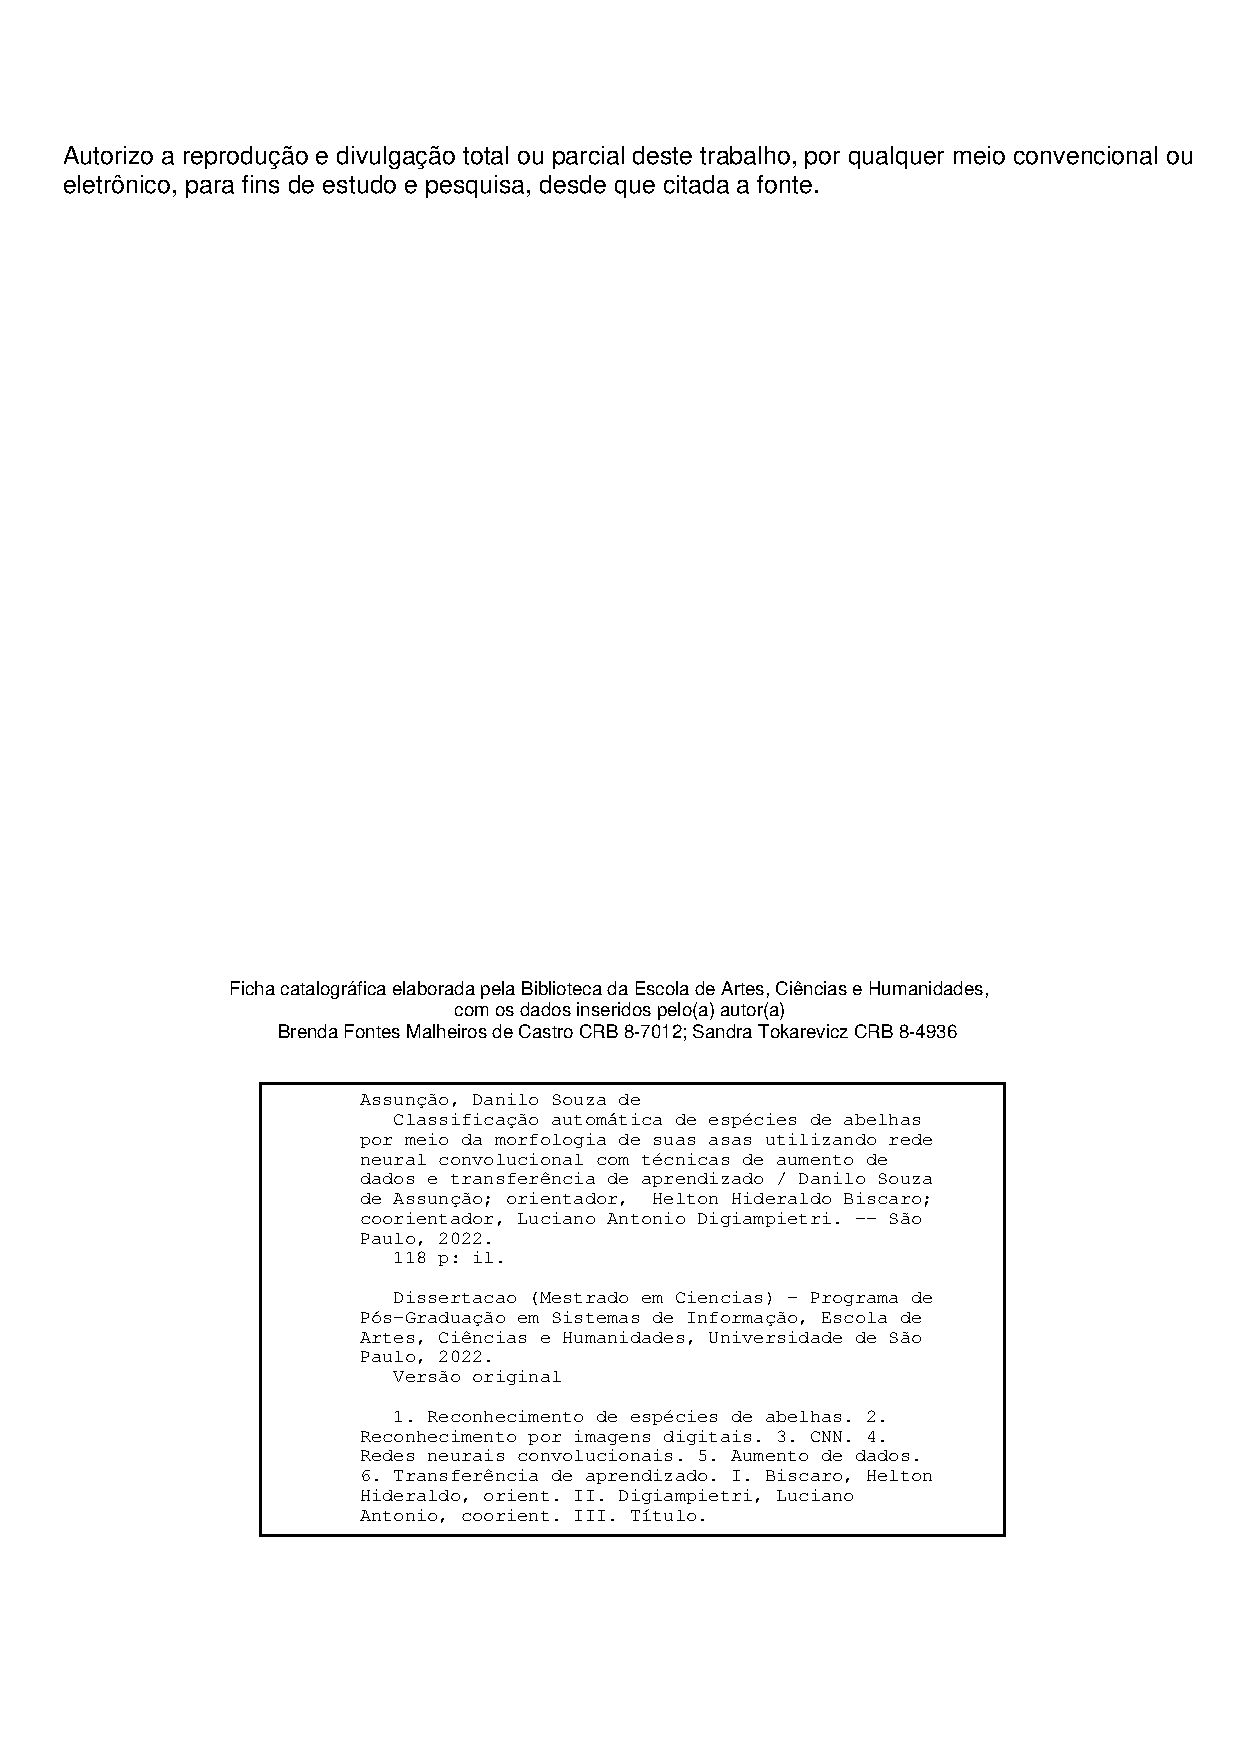
\includepdf{fig_ficha_catalografica.pdf}
\end{fichacatalografica}

% ---
% Inserir errata
% ---
%-------------------------------------------------------------------------
% Comentário adicional do PPgSI - Informações sobre ``Errata'':
%
% Usar esta página de errata apenas em casos de excepcionais, e apenas 
% para a versão corrigida da Dissertação/Tese. Por exemplo, quando depois de
% já depositada e publicada a versão corrigida, ainda assim verifica-se
% a necessidade de alguma correção adicional.
%
% Se precisar usar esta página, busque a forma correta (o modelo correto) 
% para fazê-lo, de acordo com a norma ABNT.
%
% Não usar esta página para versão original de Dissertação/Tese.
% Não usar esta página para Qualificação.
%
%-------------------------------------------------------------------------
%\begin{errata}
%Elemento opcional para versão corrigida, depois de depositada.
%\end{errata}
% ---

% ---
% Inserir folha de aprovação
% ---

\begin{folhadeaprovacao}
%-------------------------------------------------------------------------
% Comentário adicional do PPgSI - Informações sobre ``Folha da aprovação'':
%
% Página a ser usada apenas para Dissertação/Tese.
%
% Não usar esta página para Qualificação.
%
% Substituir ``Fulano de Tal'' pelo nome completo do autor do trabalho, com 
% apenas as iniciais em maiúsculo.
%
% Substituir ``___ de ______________ de ______'' por: 
%     - Para versão original de Dissertação/Tese: deixar em branco, pois a data 
%       pode mudar, mesmo que ela já esteja prevista.
%     - Para versão corrigida de Dissertação/Tese: usar a data em que a defesa 
%       efetivamente ocorreu.
%
% Para Tese de Doutorado: trocar "Dissertação" por "Tese".
%-------------------------------------------------------------------------
\noindent Dissertação de autoria de Danilo Souza de Assunção, sob o título \textbf{``\imprimirtitulo''}, apresentada à Escola de Artes, Ciências e Humanidades da Universidade de São Paulo, para obtenção do título de Mestre em Ciências pelo Programa de Pós-graduação em Sistemas de Informação, na área de concentração Metodologia e Técnicas da Computação, aprovada em \rule{0.85cm}{0.5pt} de \rule{3.5cm}{0.5pt} de \rule{1.25cm}{0.5pt} pela comissão julgadora constituída pelos doutores:

\vspace*{3cm}

\begin{center}
%-------------------------------------------------------------------------
% Comentário adicional do PPgSI - Informações sobre ``assinaturas'':
%
% Para versão original de Dissertação/Tese: deixar em 
% branco (ou seja, assim como está abaixo), pois os membros da banca podem
% mudar, mesmo que eles já estejam previstos.
% 
% Para versão corrigida de Dissertação/Tese: usar os dados dos examinadores que 
% efetivamente participaram da defesa. 
% 
% Para versão corrigida de Dissertação/Tese: em caso de ``professora'', trocar 
% por ``Profa. Dra.'' 
% 
% Para versão corrigida de Dissertação/Tese: ao colocar os nomes dos 
% examinadores, usar seus nomes completos, exatamente conforme constam em 
% seus Currículos Lattes
% 
% Para a versão corrigida de Dissertação/Tese: remova o texto “Instituição: ”, 
% ou seja, coloque apenas/diretamente o nome da instituição, por exemplo 
% "Universidade de São Paulo" ou "Universidade Estadual de Campinas".
%
% Não abreviar os nomes das instituições.
%
% Verifique quantos membros há em sua banca, de acordo com o seu regulamento, 
% especificamente para o caso de Dissertação de Mestrado ou Tese de Doutorado, 
% e use o número correto de espaços para assinaturas.
%
%-------------------------------------------------------------------------

\assinatura{Prof. Dr. \\ Instituição \\ Presidente}

\assinatura{Prof. Dr. \\ Instituição}

\assinatura{Prof. Dr. \\ Instituição}

%\assinatura{Prof. Dr. \\ Instituição}    % Incluir para bancas de tese de doutorado

%\assinatura{Prof. Dr. \\ Instituição}    % Incluir para bancas de tese de doutorado

\end{center}
  
\end{folhadeaprovacao}
% ---

% ---
% Dedicatória
% ---
%-------------------------------------------------------------------------
% Comentário adicional do PPgSI - Informações sobre ``Dedicatória'': 
%
% Opcional para Dissertação/Tese.
% Não sugerido para Qualificação.
% 
%-------------------------------------------------------------------------
\begin{dedicatoria}
  \vspace*{\fill}
  \centering
  \noindent
  \textit{Dedico este trabalho aos meus familiares, em especial a minha mãe Alessandra Marcia de Souza que esteve sempre ao meu lado me apoiando nesta trajetória.} 
	 \vspace*{\fill}
\end{dedicatoria}
% ---

% ---
% Agradecimentos
% ---
%-------------------------------------------------------------------------
% Comentário adicional do PPgSI - Informações sobre ``Agradecimentos'': 
%
% Opcional para Dissertação/Tese.
% Não sugerido para Qualificação.
% 
% 
% Financiamentos recebidos durante o projeto de mestrado/doutorado, vindos de qualquer 
% agência de fomento, devem ser mencionados na seção de agradecimentos da dissertação/tese. 
% Isso se aplica não apenas a bolsas de estudo, mas a qualquer tipo de financiamento, 
% tais como para apoio a participação em eventos, compra de materiais, traduções etc. 
% Especificamente para financiamento da Capes, siga as instruções contidas na portaria 
% 206, de 4/set/2018; para outras agências de fomento, procure as regras apropriadas.
%
% Portaria Capes 206, de 4/set/2018: 
% http://ppgsi.each.usp.br/arquivos/Portaria_0783227_Portaria_CAPES_DOU___206_de_2018.pdf 
%
%
%-------------------------------------------------------------------------
\begin{agradecimentos}
Primeiramente, eu desejo agradecer à minha mãe, Alessandra Marcia de Souza, sendo a minha melhor companhia em todo o trajeto pelo qual eu percorri neste mestrado, ela esteve comigo, me incentivando e apoiando, e isso tudo foi concluído graças à força que ela constantemente me forneceu.

À minha família, pai, irmãos, tios e avós que também me apoiaram bastante durante todo este percurso, principalmente ao meu tio, William Assunção, sendo uma das pessoas que mais me induziram a entrar no meio acadêmico.

Um reconhecimento especial aos meus orientadores, Prof. Dr. Helton Hideraldo Biscaro e Prof. Dr. Luciano Antonio Digiampietri que foram figuras excepcionais para mim, ao Helton por ter me aceitado como um dos seus orientandos, me ajudando muito durante todo o desenvolvimento do trabalho e aos ensinamentos por ele dados a mim, e ao Luciano que foi o facilitador em todo o meu processo de entrada neste programa de mestrado e também uma das pessoas que mais me auxiliou durante todo este percurso. Aos dois, meus mestres, meu eterno agradecimento.

Ao meu amigo Gilson Clemente, que me ajudou muito durante todo o desenvolvimento do meu trabalho, tendo participado em opiniões gerais em todo o escopo presente neste documento, como também um grande revisor. E também um agradecimento especial à Sammy, que é uma pessoa muito importante na minha vida.

E por fim, ao PPGSI, sendo o programa que tornou tudo isto possível, permitindo que eu participasse deste grande percurso, aprendi muito, e aqui estou, muito mais avançado do que quando comecei. Para todos os colaboradores que fazem parte deste programa, meus agradecimentos.
\end{agradecimentos}

% ---
% Epígrafe
% ---
%-------------------------------------------------------------------------
% Comentário adicional do PPgSI - Informações sobre ``Epígrafe'': 
%
% Opcional para Dissertação/Tese.
% Não sugerido para Qualificação.
% 
%-------------------------------------------------------------------------
\begin{epigrafe}
    \vspace*{\fill}
	\begin{flushright}
		\textit{``Nada é permanente, exceto a mudança.''\\
		(Heráclito)}
	\end{flushright}
\end{epigrafe}
% ---

% ---
% RESUMOS
% ---

% resumo em português
\setlength{\absparsep}{18pt} % ajusta o espaçamento dos parágrafos do resumo
\begin{resumo}

%-------------------------------------------------------------------------
% Comentário adicional do PPgSI - Informações sobre ``referência'':
% 
% Troque os seguintes campos pelos dados de sua Dissertação/Tese (mantendo a 
% formatação e pontuação):
%   - SOBRENOME
%   - Nome1
%   - Nome2
%   - Nome3
%   - Título do trabalho: subtítulo do trabalho
%   - AnoDeDefesa
%
% Mantenha todas as demais informações exatamente como estão.
% 
% [Não usar essas informações de ``referência'' para Qualificação]
%
% Para Tese de Doutorado: trocar "Dissertação (Mestrado em Ciências)" por "Tese (Doutorado em Ciências)".
%-------------------------------------------------------------------------
\begin{flushleft}
ASSUNÇÃO, Danilo Souza. \textbf{\imprimirtitulo}. \imprimirdata. \pageref{LastPage} f. Dissertação (Mestrado em Ciências) – Escola de Artes, Ciências e Humanidades, Universidade de São Paulo, São Paulo, 2022.
\end{flushleft}

O processo de classificação de espécies de abelhas é uma atividade importante para a preservação das abelhas, pois possibilita o estabelecimento de estratégias mais precisas de conservação ao obter informações detalhadas de uma determinada espécie numa localidade específica. A realização automática da análise estatística da morfologia das abelhas se convém devido às despesas necessárias nos processos de identificação manual, e, para esta análise morfológica, o conjunto de características extraídos a partir das asas têm se mostrado uma eficiente maneira para a identificação das espécies utilizando métodos estatísticos ou computacionais. O aprendizado profundo tem sido amplamente aplicado em atividades relacionadas à visão computacional. Diferente dos métodos tradicionais de aprendizado de máquina, o modelo de aprendizado profundo pode aprender características automaticamente a partir de uma grande quantidade de instâncias de dados, e não requer a assistência de um especialista no domínio para a extração destas características. No aprendizado profundo, as Redes Neurais Convolucionais (CNN) são bem conhecidas por seu sucesso em muitas tarefas de visão computacional. Neste trabalho foi desenvolvido um método utilizando CNN para classificação de espécies de abelhas através da morfologia de suas asas através do auxílio de técnicas de aumento de dados e transferência de aprendizado. A solução desenvolvida atingiu resultados superiores a 97\% para acurácia e medida F.

Palavras-chaves: Redes Neurais Convolucionais. CNN. Aumento de dados. Transferência de aprendizado. Reconhecimento de espécies. Reconhecimento de espécies de abelhas. Morfologia das asas. Reconhecimento por imagens digitais.
\end{resumo}

% resumo em inglês
%-------------------------------------------------------------------------
% Comentário adicional do PPgSI - Informações sobre ``resumo em inglês''
% 
% Caso a Qualificação ou a Dissertação/Tese inteira seja elaborada no idioma inglês, 
% então o ``Abstract'' vem antes do ``Resumo''.
% 
%-------------------------------------------------------------------------
\begin{resumo}[Abstract]
\begin{otherlanguage*}{english}

%-------------------------------------------------------------------------
% Comentário adicional do PPgSI - Informações sobre ``referência em inglês''
% 
% Troque os seguintes campos pelos dados de sua Dissertação/Tese (mantendo a 
% formatação e pontuação):
%     - SURNAME
%     - FirstName1
%     - MiddleName1
%     - MiddleName2
%     - Work title: work subtitle
%     - DefenseYear (Ano de Defesa)
%
% Mantenha todas as demais informações exatamente como estão.
%
% [Não usar essas informações de ``referência'' para Qualificação]
%
%-------------------------------------------------------------------------
\begin{flushleft}
ASSUNÇÃO, Danilo. \textbf{\imprimirtitulo}. \imprimirdata. \pageref{LastPage} p. Dissertation (Master of Science) – School of Arts, Sciences and Humanities, University of São Paulo, São Paulo, 2022.
\end{flushleft}

Bees' species classification process turns out to be an important activity in bee preservation, as it makes it possible to establish more precise conservation strategies when obtaining detailed information about a specific species and also for a specific location. The automatic realization of the visual analysis of the morphology of the bees is convenient due to the necessary expenses in the processes of manual identification, and, for this morphological analysis, the sets of characteristics extracted from the wings have shown to be an efficient way for the identification of the species using statistical methods. Deep learning has been widely applied in activities related to computer vision. Unlike traditional machine learning methods, the deep learning model can automatically learn resources from a large number of data samples and does not require the assistance of an expert in the field to extract these characteristics. In deep learning, Convolutional Neural Networks (CNN) are well known for their success in many computer vision tasks. In this work, a method was developed using CNN to classify bee species through the morphology of their wings using data augmentation and transfer learning techniques. The developed solution achieved results above 97\% for accuracy and F score.

Keywords: Convolutional Neural Networks. CNN. Data augmentation. Transfer learning. Species recognition. Recognition of bee species. Wing morphology. Digital image recognition.
\end{otherlanguage*}
\end{resumo}

% ---
% ---
% inserir lista de figuras
% ---
\pdfbookmark[0]{\listfigurename}{lof}
\listoffigures*
\cleardoublepage
% ---

% ---
% inserir lista de algoritmos
% ---
% \pdfbookmark[0]{\listalgorithmname}{loa}
% \listofalgorithms
% \cleardoublepage

% ---
% inserir lista de quadros
% ---
\pdfbookmark[0]{\listofquadrosname}{loq}
\listofquadros*
\cleardoublepage


% ---
% inserir lista de tabelas
% ---
\pdfbookmark[0]{\listtablename}{lot}
\listoftables*
\cleardoublepage
% ---

% ---
% inserir lista de abreviaturas e siglas
% ---
%-------------------------------------------------------------------------
% Comentário adicional do PPgSI - Informações sobre ``Lista de abreviaturas 
% e siglas'': 
%
% Opcional.
% Uma vez que se deseja usar, é necessário manter padrão e consistência no
% trabalho inteiro.
% Se usar: inserir em ordem alfabética.
%
%-------------------------------------------------------------------------
\begin{siglas}
  \item[ANN] Artificial Neural Network
  \item[CNN] Convolutional Neural Network
  \item[GAN] Generative Adversarial Networks
  \item[KNN] K-Nearest Neighbors
  \item[MNIST] Modified National Institute of Standards and Technology
  \item[RBF] Radius Basis Function
  \item[ReLU] Rectified Linear Unit
  \item[RGB] Red, Green and Blue
  \item[ResNet] Residual Neural Network
  \item[SGD] Stochastic Gradient Descent
  \item[SVM] Support Vector Machine
  \item[VGG] Visual Geometry Group
\end{siglas}
% ---

% ---
% inserir lista de símbolos
% ---
%-------------------------------------------------------------------------
% Comentário adicional do PPgSI - Informações sobre ``Lista de símbolos'': 
%
% Opcional.
% Uma vez que se deseja usar, é necessário manter padrão e consistência no
% trabalho inteiro.
% Se usar: inserir na ordem em que aparece no texto.
% 
%-------------------------------------------------------------------------
\begin{comment}
\begin{simbolos}

\end{simbolos}
\end{comment}
% ---

% ---
% inserir o sumario
% ---
\pdfbookmark[0]{\contentsname}{toc}
\tableofcontents*
\cleardoublepage
% ---



% ----------------------------------------------------------
% ELEMENTOS TEXTUAIS
% ----------------------------------------------------------
\textual



%-------------------------------------------------------------------------
% Comentário adicional do PPgSI - Informações sobre ``títulos de seções''
% 
% Para todos os títulos (seções, subseções, tabelas, ilustrações, etc.):
%
% Em maiúscula apenas a primeira letra da sentença (do título), exceto 
% nomes próprios, geográficos, institucionais ou Programas ou Projetos ou
% siglas, os quais podem ter letras em maiúscula também.
%
%------------------------------------------------------------------------

% ----------------------------------------------------------
% CAPITULO - INTRODUÇÃO
% ----------------------------------------------------------
\chapter{Introdução}
A partir da definição dos serviços ecossistêmicos, que designa sobre o funcionamento normal dos ecossistemas e os benefícios que as pessoas adquirem dele, tem-se uma conexão direta com a prosperidade da civilização humana. Tendo como essencialidade a polinização, sendo um dos serviços ecossistêmicos que traz segurança alimentar, mas é afetada desde a Revolução Industrial com as enormes perdas de biodiversidades que o mundo vem vivenciando \cite{rockstrom2009safe}. O valor de mercado anual dos serviços de polinização foi estimado em US\$ 235 bilhões em todo o mundo \cite{potts2016assessment}. Sendo as abelhas as polinizadoras primárias de culturas e ecossistemas naturais e, responsáveis pela reprodução da grande maioria das plantas com flores, tornando-as organismos essenciais tanto em termos econômicos quanto ecológicos, além de serem vitais para fins de conservação \cite{rebelo2021fully}.

Diferentes abordagens automáticas têm sido desenvolvidas com o objetivo de identificar automaticamente a espécie de diferentes seres vivos de forma a auxiliar a minimizar os problemas relacionados com os gastos econômicos e, principalmente, pelas perdas de biodiversidades dos ecossistemas. Estas abordagens envolvem, por exemplo, o código de barras de DNA e o reconhecimento automático de espécies com base na morfologia das asas, sendo que, estas metodologias são vantajosas por permitirem o acesso à identificação de espécies a um público mais amplo, deixando os taxonomistas despendidos em tarefas mais urgentes, como a descrição de espécies \cite{rebelo2021fully}. Vale ressaltar que, para algumas espécies, a identificação automática pode ser um desafio, principalmente para as abelhas sem ferrão que possuem características muito parecidas entre as espécies de mesmo grupo \cite{francoy2010morfometria}

Atualmente, a realização automática da análise visual da morfologia das abelhas é mais proveitosa diante das dificuldades encontradas nos processos de identificação manual, e para tal automatização da análise morfológica, os conjuntos de características extraídos a partir das asas têm se mostrado uma maneira eficiente para a identificação das espécies utilizando métodos estatísticos \cite{francoy2008identification}.

Baseado no problema abordado, em conjunto com suas possíveis soluções, alguns experimentos utilizando métodos tradicionais de aprendizado de máquina já foram realizados no trabalho de \citeonline{rebelo2021fully}, onde é feito o uso de um conjunto de técnicas de pré-processamento e segmentação de imagens, podendo ser denominados como métodos \textit{handcrafted}, para a extração manual de características relevantes e situadas nas imagens de asas de abelhas, para que, assim, fosse criado um conjunto de imagens com características capazes de serem usadas em um modelo de aprendizado de máquina supervisionado utilizando o algoritmo \textit{k-nearest neighbors} (KNN).

A partir dos resultados do experimento citado, o presente projeto objetivou realizar um aprimoramento do mecanismo que realiza todo o processo de identificação automática das espécies de abelhas através das imagens de suas asas. Desta forma, foi idealizado o uso métodos de aprendizado profundo, ou, mais especificamente, o uso de Redes Neurais Convolucionais (CNN) para a construção de ferramentas que permitam classificar automaticamente tais espécies, removendo a necessidade do uso de métodos \textit{handcrafted} para a extração de características contidas nessas imagens, automatizando por completo o fluxo.

Neste contexto, na literatura, foi identificado que o aprendizado profundo tem sido amplamente utilizado em atividades relacionadas à visão computacional. O aprendizado profundo é um subconjunto do aprendizado de máquina baseado em redes neurais artificiais. Este processo de aprendizado é profundo pois a estrutura das redes neurais artificiais consiste em várias camadas, sendo estas camadas, de entrada, saída e oculta. Diferente dos métodos tradicionais de aprendizado de máquina, o modelo de aprendizado profundo pode aprender características automaticamente a partir de uma grande quantidade de dados, e não requer a assistência de um especialista no domínio para extração manual destas características, dado que, isso é extraído automaticamente através do algoritmo \cite{liu2020classification}. No campo de aprendizado profundo, as CNNs são bem reconhecidas por seu sucesso em muitas tarefas de visão computacional \cite{le2020automated}.

A CNN oferece uma abordagem que automatiza o aprendizado de características contidas em uma imagem ao utilizar grandes conjuntos de dados, que representam um domínio de interesse da aplicação \cite{gonzalez2018deep}. Devido à necessidade de uma grande quantidade de dados para o treinamento deste tipo de rede, é essencial que, para conjuntos de dados menores, tenha-se o auxílio de técnicas que permitam atingir bons resultados. Baseado nisso, foram adicionados, no presente trabalho, mecanismos de aumento de dados e/ou transferência de aprendizado, com o propósito de se obter um modelo com melhor desempenho, por meio do uso de uma CNN que irá identificar, a partir da disponibilidade de um pequeno conjunto de dados das asas de abelhas, de maneira automatizada e sem o uso de métodos \textit{handcrafted}.

\section{Hipótese}
O uso de CNN para automatização do processo de extração de características e classificação, pode trazer resultados promissores ao problema em questão, devido a sua capacidade de identificar e extrair características de alto e baixo nível, presente nas imagens. E, estes resultados podem ser auxiliados baseando-se no uso da CNN em união com as técnicas de aumento de dados e/ou técnicas de transferência de aprendizado.

Esta hipótese foi testada, levando em consideração, as medidas tradicionais de aprendizado de máquina obtidas a partir do modelo proposto, relacionando-o com o modelo de \textit{baseline} apresentado em \citeonline{rebelo2021fully}.

Espera-se que o modelo proposto apresente resultados similares ou superiores ao modelo de \textit{baseline} para as medidas sugeridas.

\section{Objetivos}
Este projeto de pesquisa tem como objetivo o desenvolvimento de uma ferramenta de classificação de espécies de abelhas por meio da morfologia de suas asas, utilizando-se de uma CNN como mecanismo de extração de características e classificação destas imagens, junto à utilização de técnicas de aumento de dados ou transferência de aprendizado para otimização dos resultados do modelo, a fim de se obter resultados relevantes, como apresentados no \textit{baseline} definido. Desta forma, este trabalho tem os seguintes objetivos específicos:

\begin{enumerate}
  \item Desenvolvimento, teste e validação de ferramenta (\textit{pipeline}) que realize automaticamente o processamento, ampliação, organização e armazenamento de conjunto de dados contendo as imagens para treinamento, validação e teste do modelo;
  \item Desenvolvimento, teste e validação de ferramenta (\textit{pipeline}) que utilize o conjunto de dados processado e disponibilizado em união a arquiteturas de CNN para experimentação dos modelos no domínio proposto.
\end{enumerate}

\section{Justificativa}
Uma vez que o modelo demonstrar cenários de sucesso com base nas avaliações e resultados extraídos, torna-se evidente que a aplicação de uma CNN poderá atingir um modelo mais próximo do estado da arte para o problema abordado.

\section{Estrutura do documento}
O restante deste documento está organizado da seguinte forma. O capítulo 2 descreve os conceitos fundamentais para o entendimento do trabalho. O capítulo 3 apresenta a revisão de literatura realizada. O capítulo 4 descreve o conjunto de dados e as técnicas a serem utilizadas. O capítulo 5 detalha a abordagem desenvolvida. O capítulo 6 apresenta os resultados e as discussões realizadas em cima destes resultados. E por fim, o capítulo 7 apresenta a conclusão deste projeto e suas possibilidades futuras.

% ----------------------------------------------------------
% CAPITULO - CONCEITOS FUNDAMENTAIS
% ----------------------------------------------------------
\chapter{Conceitos fundamentais}
Neste capítulo são apresentados alguns tópicos fundamentais para a compreensão deste projeto. Dessa forma, primeiro é realizada uma curta introdução ao tema de visão computacional, logo depois são apresentadas as definições referentes a aprendizado de máquina, aprendizado profundo, redes neurais artificiais, Redes Neurais Convolucionais (CNN), técnicas de transferência de aprendizado e aumento de dados.

\section{Visão computacional}
A Visão Computacional pode ser descrita como uma subárea da Computação Gráfica, a qual busca extrair informações relevantes das imagens. Em outras palavras, a entrada de dados é uma imagem e a saída são informações como: existe ou não determinado objeto, características ou atividade na imagem de entrada \cite{rebelo2021fully}. E a meta da visão computacional é utilizar computadores para simular a visão humana, incluindo o aprendizado e a capacidade de fazer inferências e agir com base em informações visuais. Essa área representa um ramo da inteligência artificial cujo objetivo é simular a inteligência humana \cite{gonzalez2000processamento}.

Neste contexto, conforme a definição dada por \citeonline{gonzalez2000processamento}, uma imagem pode ser estabelecida como uma função bidimensional, $f(x,y)$, em que $x$ e $y$ são coordenadas espaciais (plano), e a amplitude de $f$ em qualquer par de coordenadas $(x,y)$ é chamada de intensidade ou nível de cinza da imagem nesse ponto. Quando $x$, $y$ e os valores de intensidade de $f$ são quantidades finitas e discretas, chamamos de imagem digital. O campo do processamento digital de imagens se refere ao processamento de imagens digitais por um computador digital. Observe que uma imagem digital é composta de um número finito de elementos, cada um com localização e valor específicos. Esses elementos são chamados de elementos \textit{pictóricos}, elementos de imagem, \textit{pels} e \textit{pixels}. \textit{Pixel} é o termo mais utilizado para representar os elementos de uma imagem digital.

Para um modelo de visão computacional, tem-se, conforme demonstrado por \citeonline{gonzalez2018deep}, a composição de determinadas etapas, sendo tais etapas, aquisição, pré-processamento, extração de características e classificação. A aquisição gera os padrões brutos de entrada (por exemplo, imagens digitais); o pré-processamento trata de tarefas como redução de ruído e correções geométricas; a extração de características lida com atributos computacionais que são fundamentais para diferenciar uma classe de padrões de outra; e a classificação é o processo que atribui um determinado padrão de entrada a uma das várias classes predefinidas.

\section{Aprendizado de máquina}
Dentre as definições presentes na literatura, \citeonline{mohri2018foundations} dizem que, o aprendizado de máquina pode ser amplamente definido como métodos computacionais, usando a experiência (dados) para melhorar o desempenho ou realizar previsões precisas. A experiência se refere às informações anteriores disponíveis para o modelo de aprendizagem de máquina, que normalmente assumem a forma de dados eletrônicos coletados e disponibilizados para análise. Esses dados podem estar na forma de conjuntos de treinamento com identificação humana ou a diferentes tipos de informações obtidas por meio da interação com o ambiente. Em todos os casos, sua qualidade e tamanho são cruciais para o sucesso das previsões feitas pelo modelo. De maneira geral, as técnicas de aprendizagem são métodos orientados por dados que combinam conceitos fundamentais em ciência da computação com ideias de estatística, probabilidade e otimização.

\subsection{Principais tarefas em aplicações de aprendizado de máquina}
Nesta seção são explicados alguns conceitos sobre as tarefas de aprendizado de máquina, sendo comumente utilizados e explicados em \citeonline{mohri2018foundations}. Tais tarefas de aprendizado de máquina são:

\begin{itemize}
  \item \textbf{Classificação}: trata-se do problema de atribuir uma categoria a cada item. Por exemplo, a classificação de imagens consiste em atribuir a cada imagem uma categoria como carro, navio ou avião. O número de categorias em tais tarefas costuma ser menor do que algumas centenas, mas pode ser muito maior em algumas tarefas difíceis, e até mesmo ilimitadas, como em classificação de texto ou reconhecimento de fala.

  \item \textbf{Regressão}: é a atividade de solucionar problemas já previstos a partir de dados históricos de cada item. Exemplos de regressão incluem a previsão de valores de estoque ou índice econômicos. Na regressão, a penalidade para uma previsão incorreta depende da magnitude da diferença entre os valores verdadeiros e previstos, em contraste com o problema de classificação, em que normalmente não há noção de proximidade entre as várias categorias.

  \item \textbf{Redução de dimensionalidade}: consiste em transformar uma representação inicial de itens em uma representação de dimensão inferior, preservando algumas propriedades da representação inicial. Um exemplo comum envolve o pré-processamento de imagens digitais em tarefas de visão computacional.
\end{itemize}

\subsection{Terminologias}
Baseado nas terminologias empregadas em \citeonline{mohri2018foundations}, a seguir está uma lista de definições e terminologias habitualmente usados no escopo de aprendizado de máquina:

\begin{itemize}
  \item \textbf{Instâncias}: são unidades que representam cada dado dentro de um conjunto de dados que são usados para aprendizado e avaliação do modelo. Imaginando o problema de identificação das espécies de abelhas através da imagem de suas asas, uma instância seria o correspondente a uma imagem de uma asa de abelha dentro do conjunto de imagens presentes no conjunto de dados.
  
  \item \textbf{Características}: O conjunto de atributos, frequentemente representado como um vetor, associado a uma instância. No caso de uma imagem, algumas características relevantes podem incluir a forma do objeto presente nesta imagem, cor e dentre vários outros aspectos.
  
  \item \textbf{Rótulo ou Classe}: valores ou categorias atribuídos a exemplos. Em problemas de classificação, as instâncias são atribuídas a categorias específicas. Por exemplo, considerando imagens de objetos de veículos, se tem categorias como, carro, avião ou navio.
  
  \item \textbf{Hiperparâmetros}: parâmetros livres que não são determinados pelo algoritmo de aprendizagem, mas sim especificados como entrada para o algoritmo de aprendizagem.

  \item \textbf{Instância de treinamento}: são instâncias utilizadas para treinar um algoritmo de aprendizagem. Em um problema envolvendo reconhecimento de padrões por meio de imagens digitais, a instância de treinamento consiste em um conjunto de exemplos de imagens junto a suas classes associadas.

  \item \textbf{Instância de validação}: são exemplos usados para ajustar os parâmetros de um algoritmo de aprendizagem ao trabalhar com dados rotulados. A instância de validação é usada para selecionar valores apropriados para os parâmetros livres do algoritmo de aprendizagem (hiperparâmetros).

  \item \textbf{Instância de teste}: são exemplos usados para avaliar o desempenho de um algoritmo de aprendizagem. A instância de teste é separada dos dados de treinamento e validação, não sendo disponibilizada na fase de aprendizado. Por exemplo, em um cenário de reconhecimento facial, a instância de teste consiste em uma coleção de exemplos de imagens de rostos, para os quais o algoritmo de aprendizagem deve prever suas determinadas classes com base em certas características, sendo então comparadas com as características da instância de teste para medir o desempenho do algoritmo.

  \item \textbf{Função de perda}: em problemas de otimização, a função de perda é um tipo de função que mede o grau de previsões incorretas realizadas pelo algoritmo, ou seja, se o algoritmo apresentar uma qualidade não desejada, o valor exibido pela função de perda será alto.
\end{itemize}

\subsection{Aprendizagem supervisionada}
A aprendizagem supervisionada é um ramo do aprendizado de máquina, método de análise de dados que usa algoritmos que aprendem iterativamente a partir dos dados para permitir que os computadores encontrem informações ocultas sem serem explicitamente programados para onde procurar \cite{o2015introduction}. A aprendizagem supervisionada resolve problemas já conhecidos usando um conjunto de dados previamente rotulado para treinar um algoritmo para realizar tarefas específicas \cite{nasteski2017overview}. Ela usa modelos para prever resultados conhecidos, por exemplo, um processo de aprendizagem supervisionada poderia ser o de classificar veículos de duas e quatro rodas a partir de suas imagens. Os dados de treinamento teriam que ser rotulados corretamente para identificar se um veículo é de duas rodas ou de quatro rodas. A aprendizagem supervisionada permite que os algoritmos ``aprendam'' a partir de dados históricos de treinamento e os apliquem a entradas desconhecidas para derivar a saída correta \cite{o2015introduction}.

\subsection{Sobreajuste e subajuste}
Conforme apresentado em \citeonline{bonaccorso2017machine}, o objetivo de um modelo de aprendizado de máquina é aproximar uma função desconhecida que associe elementos de entrada aos de saída (para um classificador, os chamamos de classes) . No entanto, essa condição ideal nem sempre é fácil de se alcançar, e este comportamento ocorre devido a duas características eminentes que são:

\begin{itemize}
  \item \textbf{Sobreajuste}: ocorre quando o modelo perde sua capacidade de generalização, sendo assim, ele pode associar quase perfeitamente todas as instâncias conhecidas aos valores de saída correspondentes, mas quando uma entrada desconhecida é apresentada, o erro de previsão correspondente pode ser muito alto.

  \item \textbf{Subajuste}: ocorre quando o modelo não é capaz de determinar um padrão, sendo incapaz de determinar uma relação entre os dados e já possuindo resultados inconsistentes na fase de treinamento do modelo.
\end{itemize}

Para exemplificar estes conceitos, na Figura \ref{fig:subajuste_sobreajuste} temos como primeiro caso o cenário de subajuste, em que a linha vermelha retrata os resultados do modelo que indica a incapacidade de generalização com relação aos dados do exemplo, dado que, ele não é capaz de distinguir os elementos abordados. Na imagem do meio, temos o cenário ideal, apresentando a capacidade do modelo em gerar uma função capaz de se generalizar com o modelo proposto. Por fim é exibido o cenário de sobreajuste, em que é possível observar a linha vermelha definindo o resultado do modelo se ajustou exatamente aos exemplos propostos, entretanto, dado a inserção de novas instâncias, este modelo pode vir a apresentar altas taxas de erro.

\begin{figure}[H]
    \centering
    \caption{Representação gráfica de subajuste e sobreajuste}
    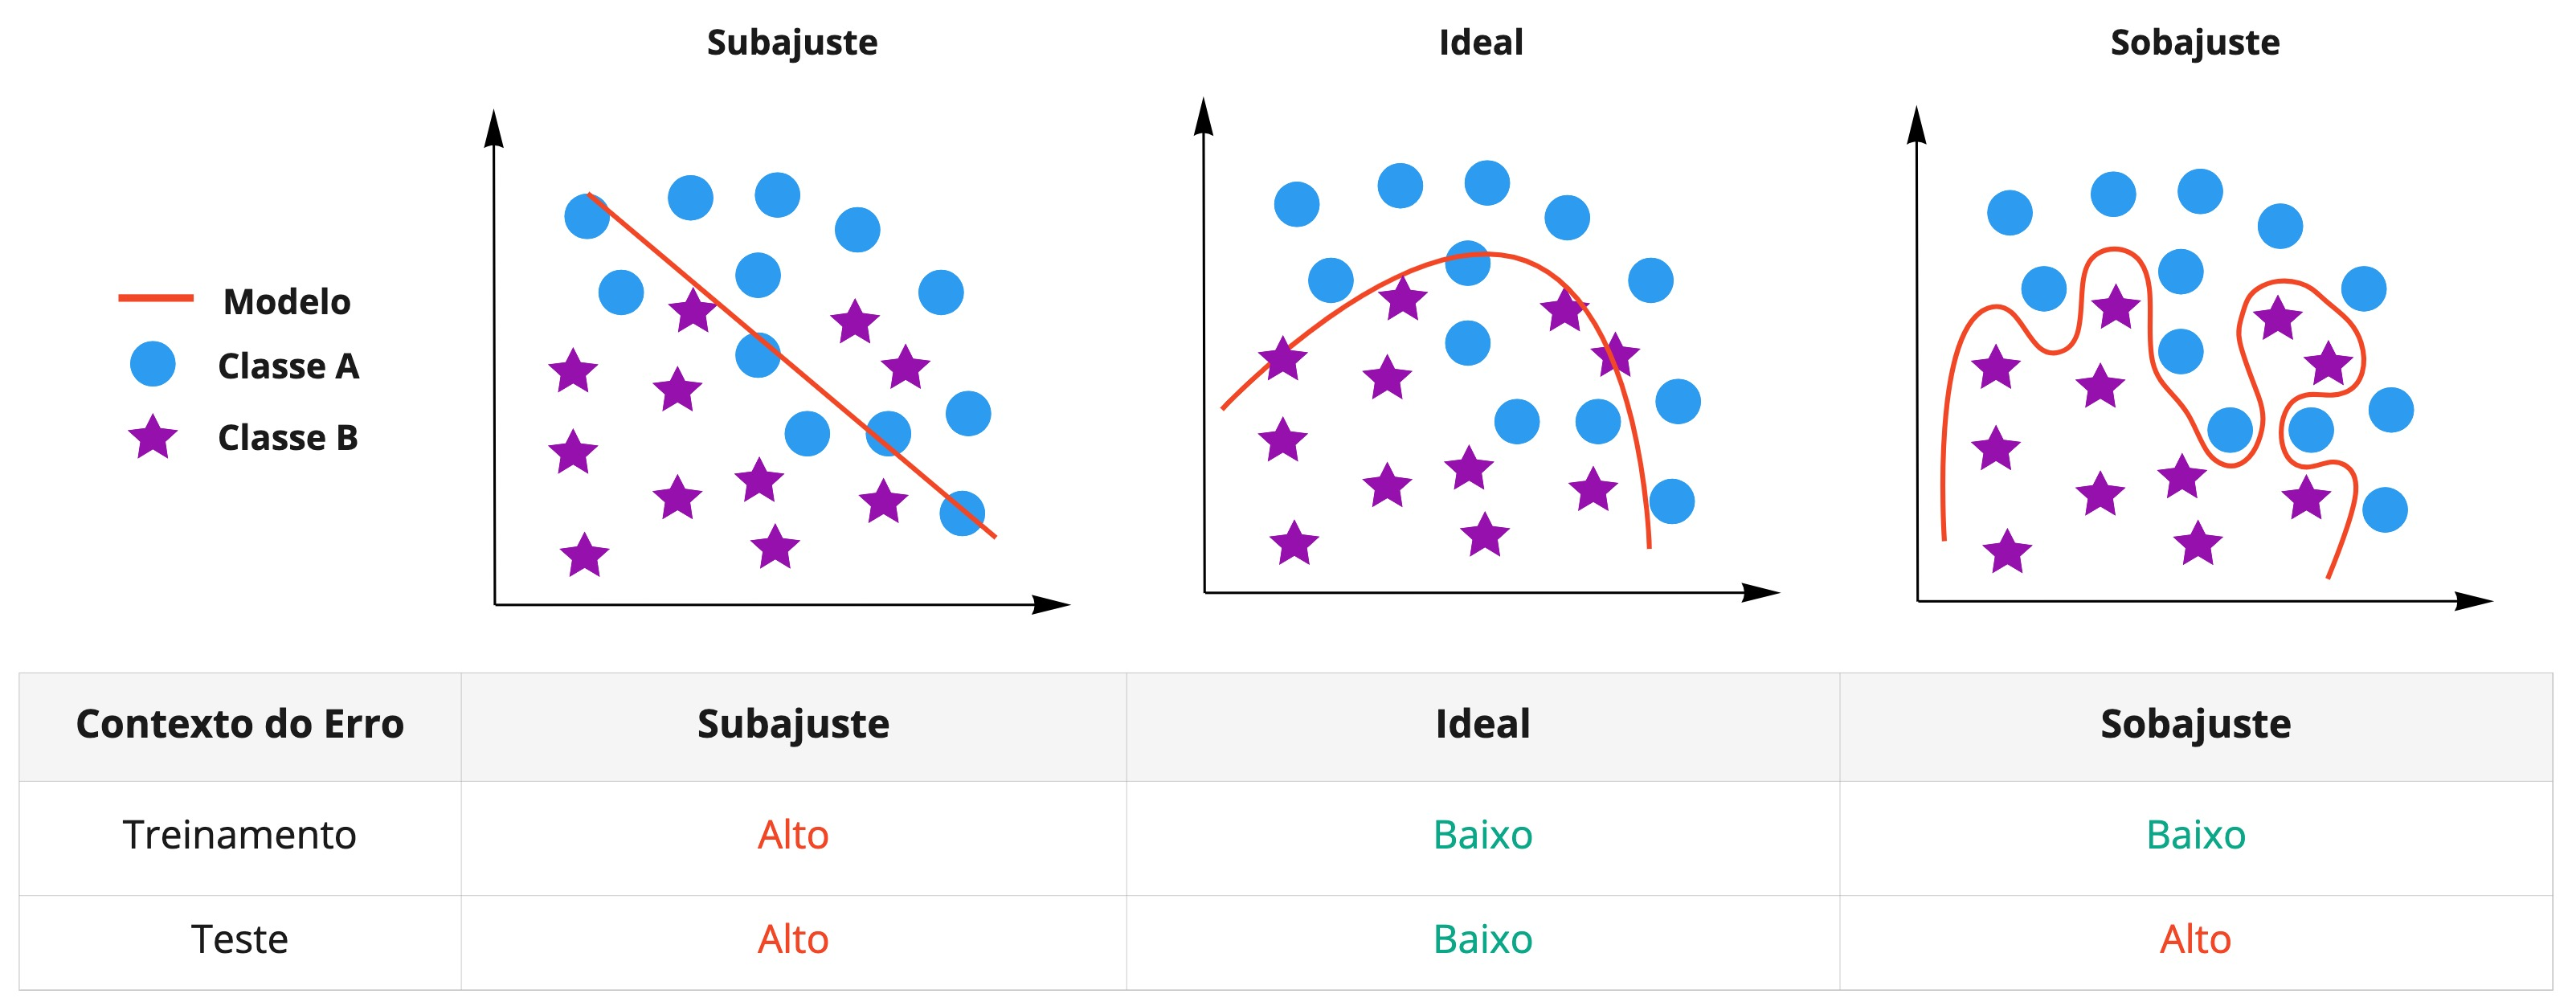
\includegraphics[width=1\textwidth]{imagens/conceitos_basicos/subajuste_sobreajuste.jpg}
    \label{fig:subajuste_sobreajuste}
    \source{Danilo Assunção, 2022}
\end{figure}

\subsection{Avaliação de desempenho de classificadores}
Ao categorizar uma instância baseada em um algoritmo de classificação, pode-se determinar que tal instância pertence a um dos quatro itens seguintes:

\begin{itemize}
  \item Verdadeiro positivo
  \item Verdadeiro negativo
  \item Falso positivo
  \item Falso negativo
\end{itemize}

Um Verdadeiro positivo é um resultado em que o modelo prevê corretamente a classe positiva. Da mesma forma, um Verdadeiro negativo é um resultado em que o modelo prevê corretamente a classe negativa. Um Falso positivo é um resultado em que o modelo prevê incorretamente a classe positiva. E um Falso negativo é um resultado em que o modelo prevê incorretamente a classe negativa.

Para fins de medição de qualidade do modelo de aprendizado de máquina, são utilizadas métricas de avaliação de classificadores. As funções mais usuais entre elas são:

\begin{itemize}
  \item Acurácia
  \item Precisão
  \item Revocação
  \item Medida F
\end{itemize}

Acurácia corresponde ao total de instâncias classificadas corretamente (independentemente da classe) dividido pelo número total de instâncias. Sua equação pode ser descrita pela Equação \ref{equation_acuracia}.

\begin{equation}
  \textit{Acurácia}=\frac{\textit{Verdadeiro positivo} + \textit{Verdadeiro negativo}}{\textit{Verdadeiro positivo} + \textit{Verdadeiro negativo} + \textit{Falso positivo} + \textit{Falso negativo}}
  \label{equation_acuracia}
\end{equation}

Precisão é a parcela de instâncias que obtiveram uma identificação e classificação corretamente. Podendo ser descrita a partir de seu cálculo pela Equação \ref{equation_precisao}.

\begin{equation} 
  \textit{Precisão}=\frac{\textit{Verdadeiro positivo}}{\textit{Verdadeiro positivo} + \textit{Falso positivo}}
  \label{equation_precisao}
\end{equation}

Revocação é a parcela de instâncias com identificação correta, em que pertencem a uma determinada classe entre todas as instâncias desta mesma classe. Seu cálculo pode ser descrito a partir da Equação \ref{equation_revocacao}.

\begin{equation}
  \textit{Revocação}=\frac{\textit{Verdadeiro positivo}}{\textit{Verdadeiro positivo} + \textit{Falso negativo}}
  \label{equation_revocacao}
\end{equation}

Medida F corresponde à média harmônica entre a precisão e a revocação. O valor da medição torna-se ideal quanto mais próximo de 1,0 (ou 100\%), enquanto que, quanto mais próximo de 0 (ou 0\%), expressa um resultado ruim. Sua equação pode ser descrita pela Equação \ref{equation_medida_f}.

\begin{equation}
  \textit{Medida F}=2 \times \frac{\textit{Precisão} \times \textit{Revocação}}{\textit{Precisão}+\textit{Revocação}}
  \label{equation_medida_f}
\end{equation}

\section{Aprendizado profundo}
Dentre as diversas definições presentes, no artigo de \citeonline{6310529}, o aprendizado profundo é sobre o aprendizado automático de vários níveis de representações da distribuição subjacente dos dados a serem modelados. Em outras palavras, um algoritmo de aprendizado profundo extrai automaticamente as características de baixo e alto nível, necessários para a classificação. Por características de alto nível, entende-se a característica que depende hierarquicamente de outras características, enquanto as características de baixo nível são detalhes únicos extraídos sucessivamente dentre as camadas da rede neural.

\subsection{Algoritmo de otimização}
Algoritmos de otimização são métodos que possibilitam a capacidade de algoritmos de aprendizado de máquina a aprenderem através de algoritmos que computam gradientes (gradiente descendente) \cite{zaheer2019study}, sendo um método que consiste em descobrir, iterativamente, os valores dos parâmetros (pesos) da rede na tentativa de minimizar a função de perda, para que assim seja maximizado o fator de previsibilidade do modelo, já que o objetivo principal deste método é diminuir o erro da rede.

No aprendizado profundo existem otimizadores de categoria adaptativa, que são denominados dessa forma pois eles usam taxas de aprendizado diferentes para cada iteração. A mudança na taxa de aprendizado depende da diferença nos parâmetros (pesos) durante o treinamento. Quanto mais os parâmetros forem alterados, menores serão as alterações na taxa de aprendizado. Essa modificação é altamente benéfica porque os conjuntos de dados do mundo real contêm características esparsas e densas, portanto, dependendo do cenário, pode não ser muito adequado ter o mesmo valor para a taxa de aprendizado para todas as características.

\section{Redes neural artificial}
As redes neurais artificiais (\textit{artificial neural networks} - ANN) são sistemas de processamento computacional que são fortemente inspirados pelo modo como os sistemas nervosos biológicos (como o cérebro humano) operam \cite{o2015introduction}. Uma rede neural consiste em muitos elementos de processamento unidos para formar uma rede apropriada com funções de ponderação ajustáveis para cada entrada. Esses elementos de processamento geralmente são organizados em uma sequência de camadas com conexões completas ou aleatórias entre as camadas. Normalmente, existem três ou mais camadas, uma camada de entrada onde os dados são apresentados, uma ou mais camadas intermediárias ou ocultas e uma camada de saída contendo a resposta de saída para uma determinada entrada \cite{483329}. A estrutura básica de uma ANN pode ser modelada como mostrado na Figura \ref{fig:artificial_neural_networks_arch}. 

\begin{figure}[H]
    \centering
    \caption{Arquitetura simplificada de uma rede neural artificial}
    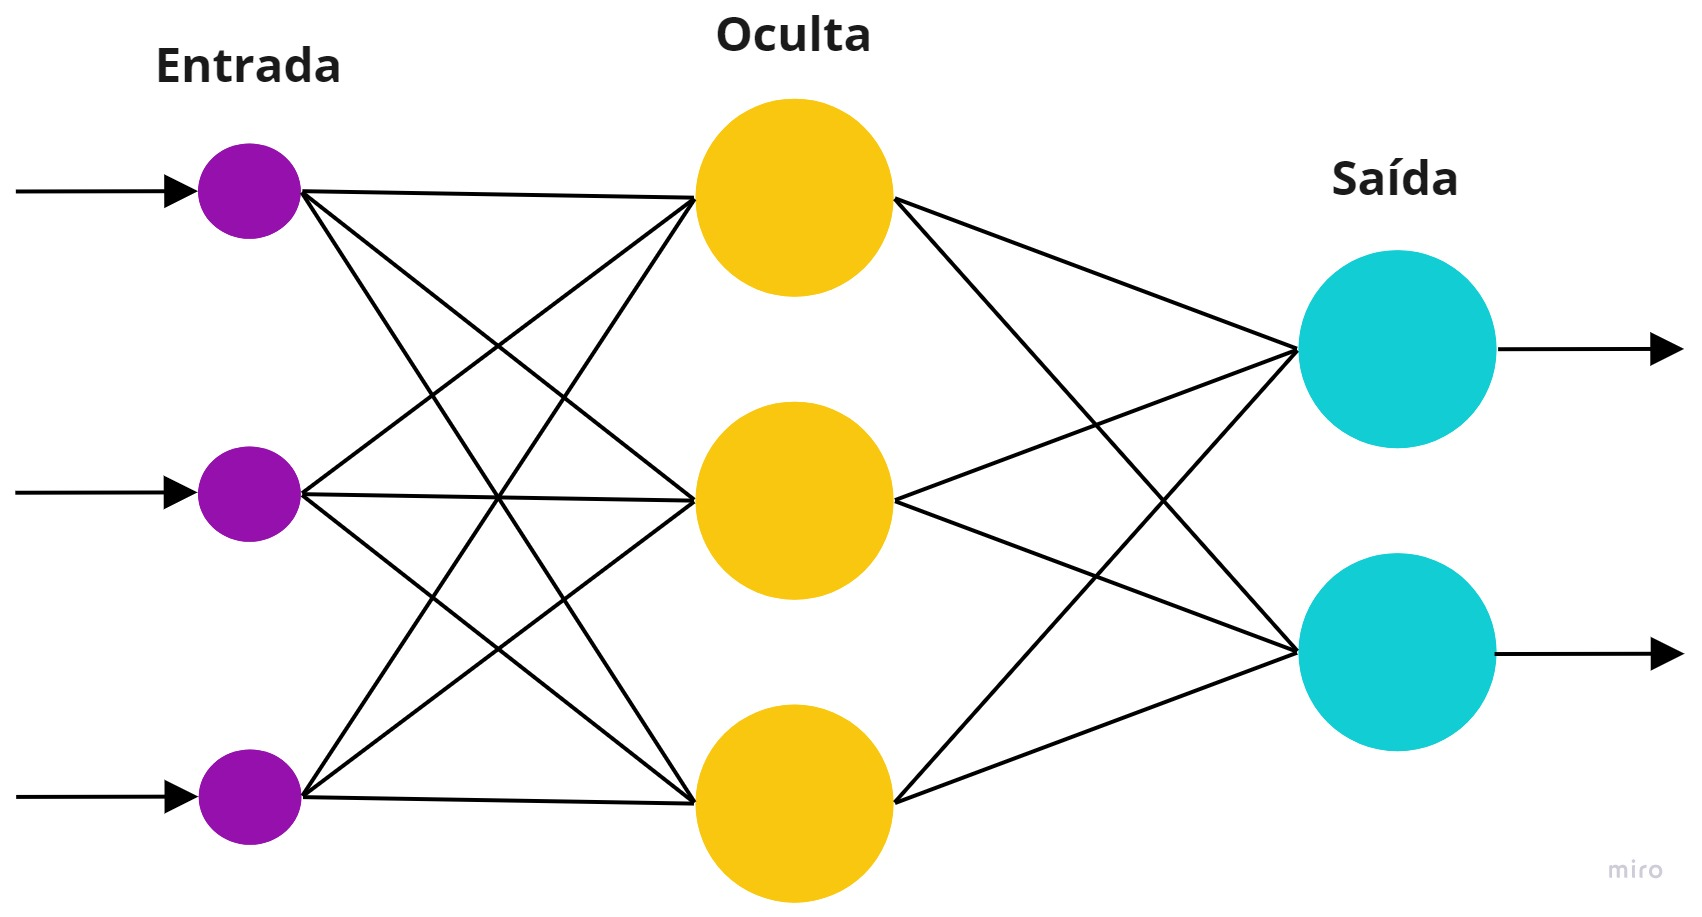
\includegraphics[scale=.20]{imagens/conceitos_basicos/rede_neural_artificial.jpg}
    \label{fig:artificial_neural_networks_arch}
    \source{Danilo Assunção, 2022}
\end{figure}

\section{Redes Neurais Convolucionais}
Baseado na definição em \citeonline{yamashita2018convolutional}, a Rede Neural Convolucional (CNN) é uma técnica de aprendizado profundo para o processamento de dados, inspirada na organização do córtex visual animal e projetada para aprender, de forma automática e adaptativa, as características de baixo e alto nível disponíveis nas imagens. A CNN normalmente é composta por dois grupos de trabalho, o primeiro grupo é o responsável pelo processo de extração de características dos dados de entrada (imagens), e o segundo grupo tem a responsabilidade de efetuar a classificação a partir dos dados extraídos do primeiro grupo. O primeiro grupo possui duas camadas principais, sendo elas, a convolução (\textit{convolutional layer}) e o agrupamento (\textit{pooling layer}) e, no último grupo, é tido a camada totalmente conectada (\textit{fully-connected layer}). Estas representações podem ser visualizadas de maneira macro através da Figura \ref{fig:arquitetura_macro_cnn}.

\begin{figure}[H]
    \centering
    \caption{Arquitetura macro de uma CNN}
    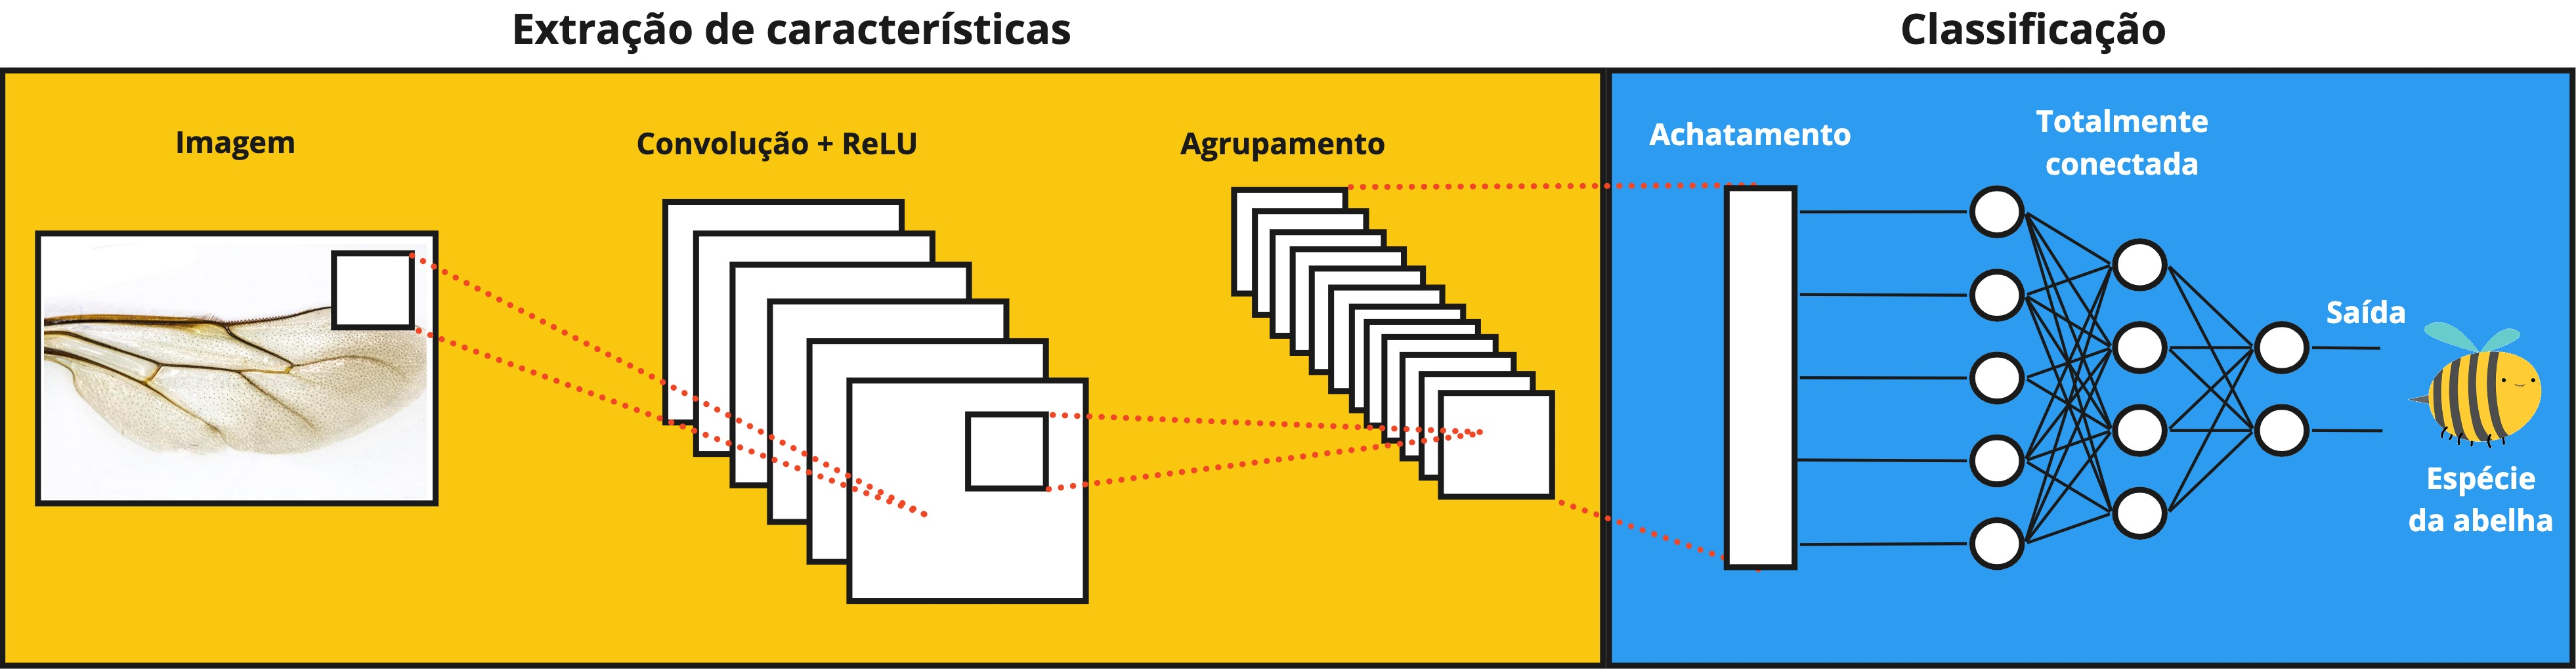
\includegraphics[width=1.0\textwidth]{imagens/conceitos_basicos/arquitetura_cnn.jpg}
    \label{fig:arquitetura_macro_cnn}
    \source{Danilo Assunção, 2022}
\end{figure}

As camadas de convolução e agrupamento executam a extração de características, enquanto a camada totalmente conectada mapeia as características extraídas na saída final, como a classificação.

\subsection{Camada convolucional}
A camada convolucional (\textit{convolutional layer}) é um componente fundamental da arquitetura de uma CNN, tendo como objetivo a extração de características de uma imagem digital, que consiste normalmente em uma combinação de operações matemáticas para se realizar tal tarefa \cite{yamashita2018convolutional}.

De acordo com as definições em \citeonline{o2015introduction}, a convolução pode ser tratada como um tipo especializado de operação linear, usada para o processo de extração de características em que, um filtro pequeno em dimensionalidade espacial é aplicado em uma matriz de valores (imagem) que se espalha ao longo de toda a profundidade da entrada. Quando uma imagem atinge uma camada convolucional, esta camada \textit{convoluciona} cada filtro na imagem, para assim produzir um mapa de características. Conforme o filtro é navegado pela imagem, o produto escalar é calculado para cada valor do filtro, como é mostrado na Figura \ref{fig:convolution_cnn}. A partir disso, na camada convolucional, a rede aprenderá os filtros que serão excitados (ativados) quando veem uma característica específica em uma determinada posição espacial da imagem.

\begin{figure}[H]
    \centering
    \caption{Processo da convolução em dados de entrada}
    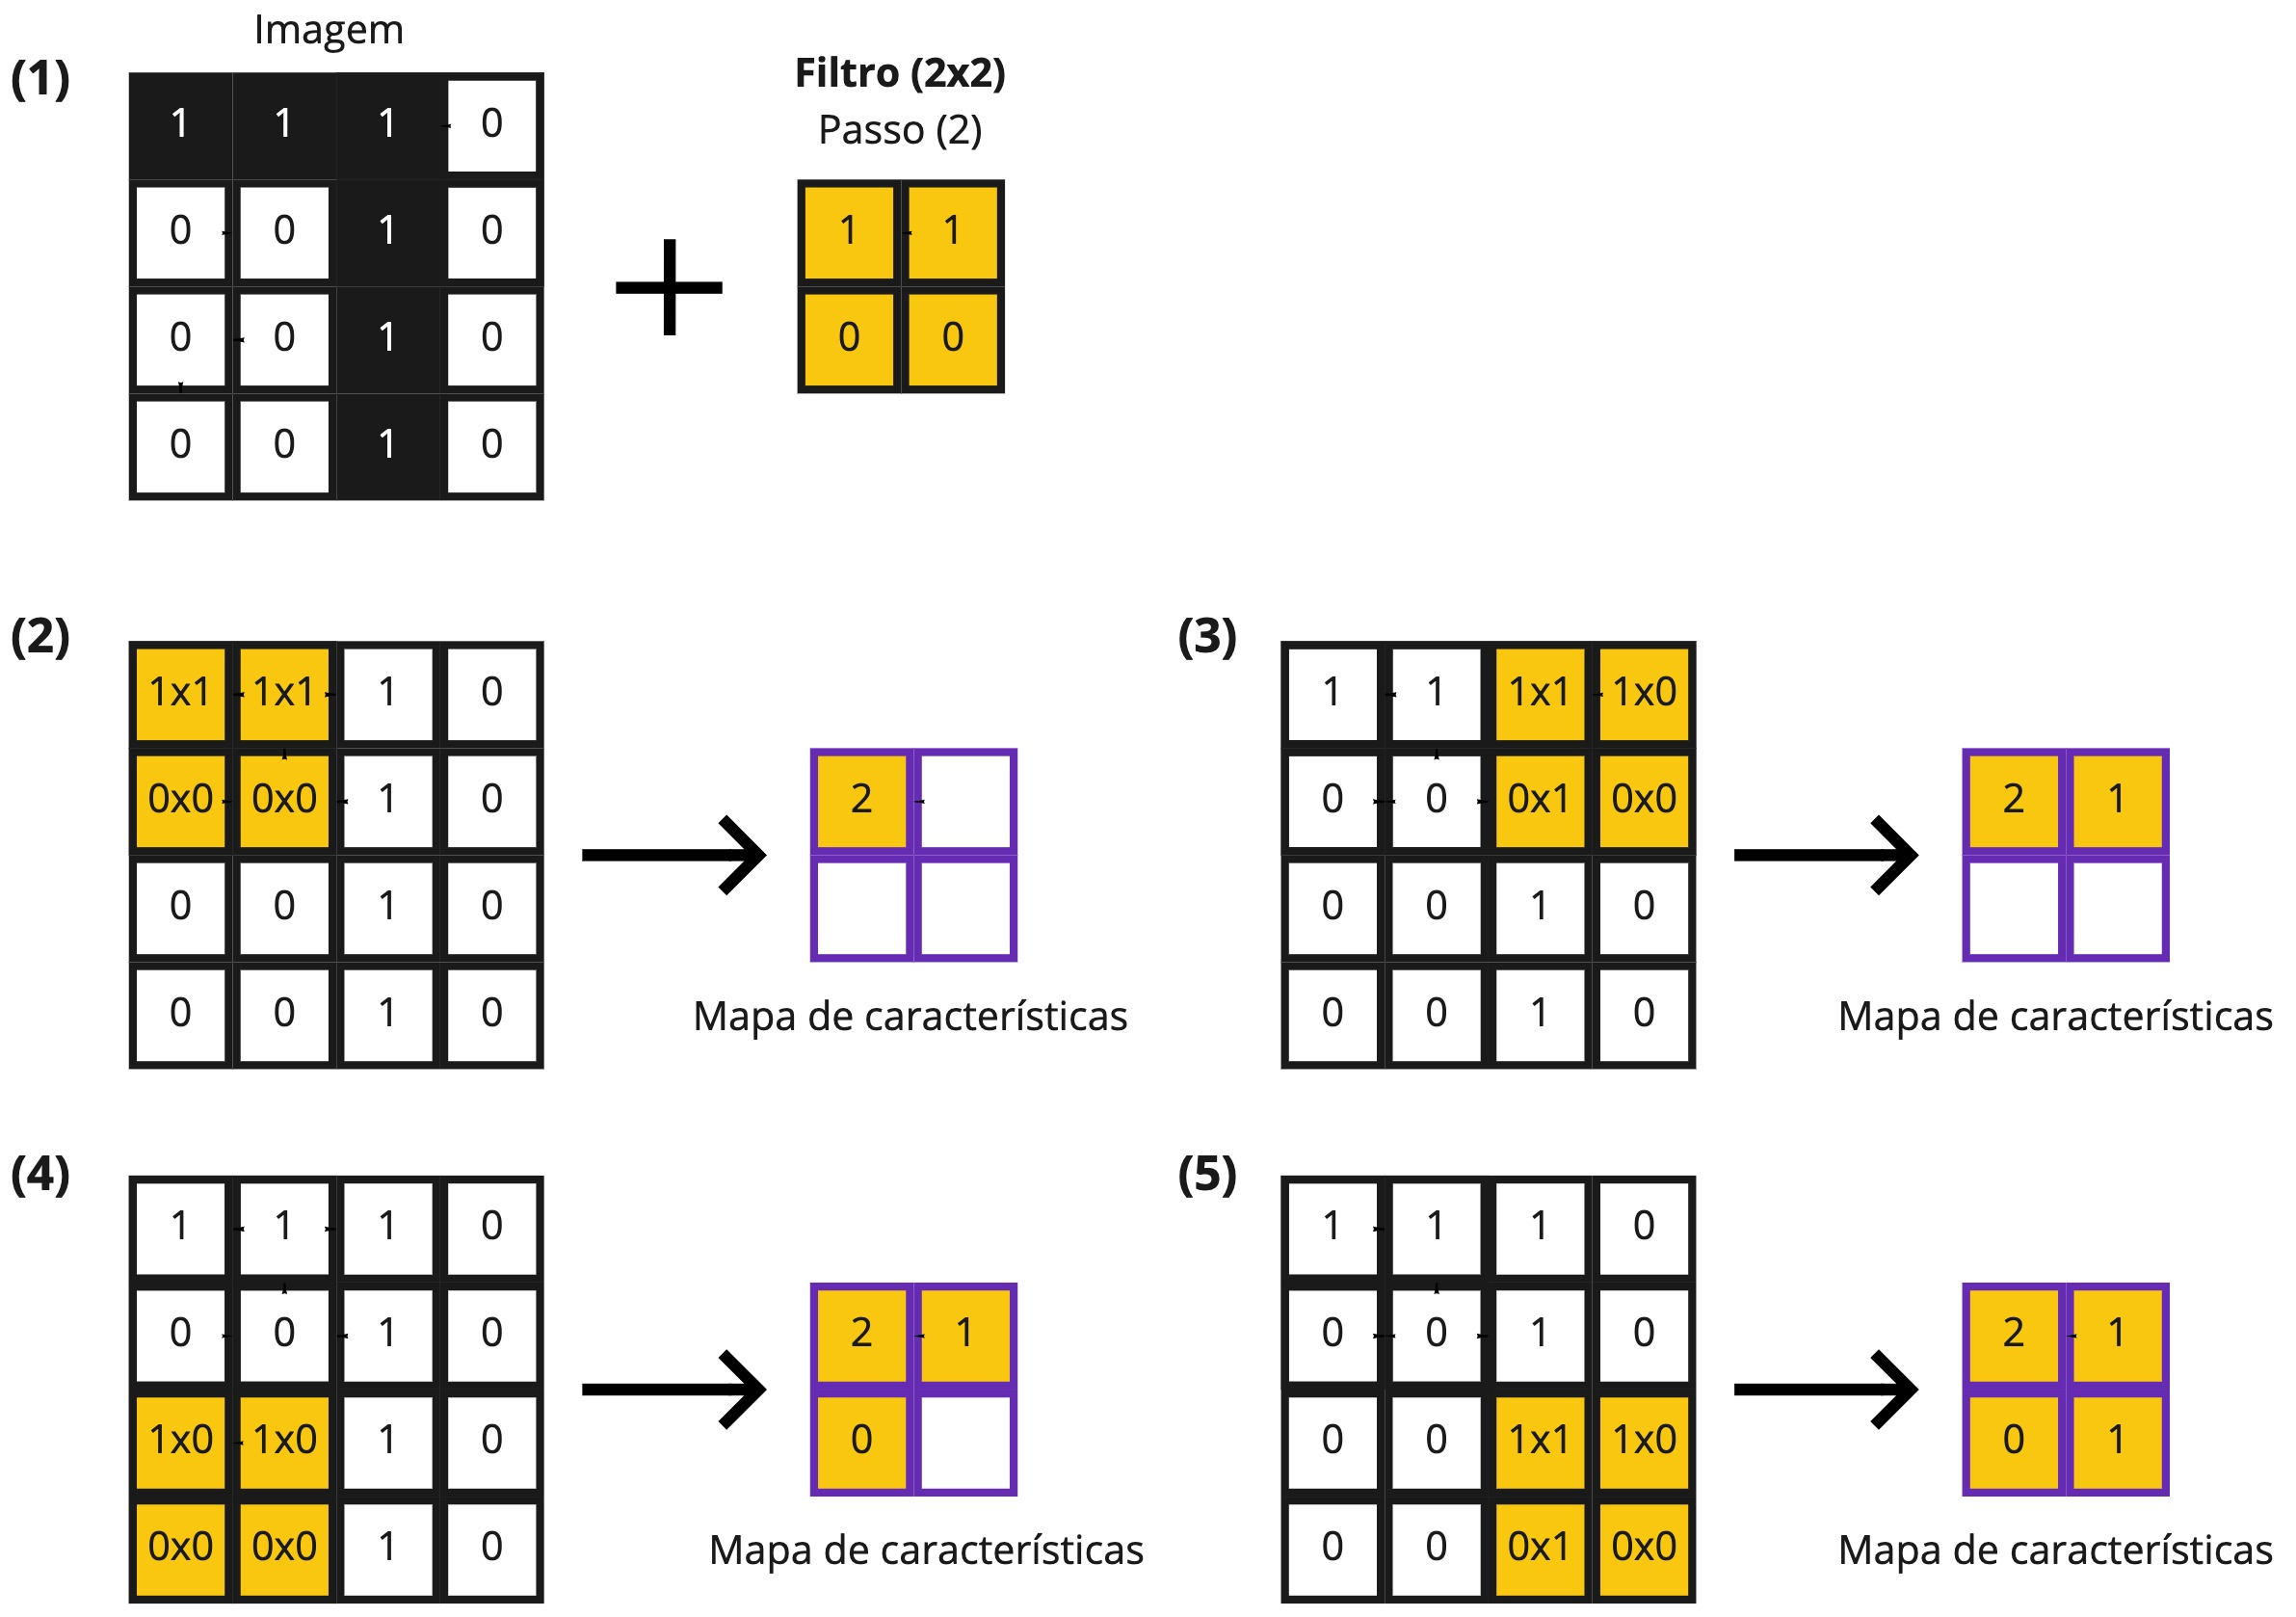
\includegraphics[width=1.0\textwidth]{imagens/conceitos_basicos/convolution.jpg}
    \label{fig:convolution_cnn}
    \source{Danilo Assunção, 2022}
\end{figure}

Nas definições em \citeonline{o2015introduction}, o filtro de convolução possui alguns hiperparâmetros importantes, sendo os principais, dimensão espacial do filtro, passo (\textit{stride}) e o preenchimento (\textit{padding}).

A dimensão espacial do filtro é definida proporcionando valores que definem o aspecto de dimensão do filtro para convolução, podendo assumir uma dimensão de 3x3, entretanto filtros de 5x5 ou 7x7 também podem ser usados. Este tamanho vai de acordo com a aplicabilidade, ou com o domínio abordado.

O passo especifica o quanto movemos o filtro de convolução em cada etapa. Ou seja, se definíssemos o valor do passo como 1, teríamos um campo receptivo (filtro) sendo envolvido em passos de 1 da esquerda para a direita e de cima para baixo por toda a dimensão espacial da imagem. Alternativamente, definir o passo para um número maior, reduzirá a quantidade de sobreposição e produzirá uma saída de dimensões espaciais menores. Na Figura \ref{fig:convolution_stride_cnn} é demonstrado um exemplo usando um passo de valor 2.

\begin{figure}[H]
    \centering
    \caption{Exemplo do uso do passo de valor 2 no processo convolucional}
    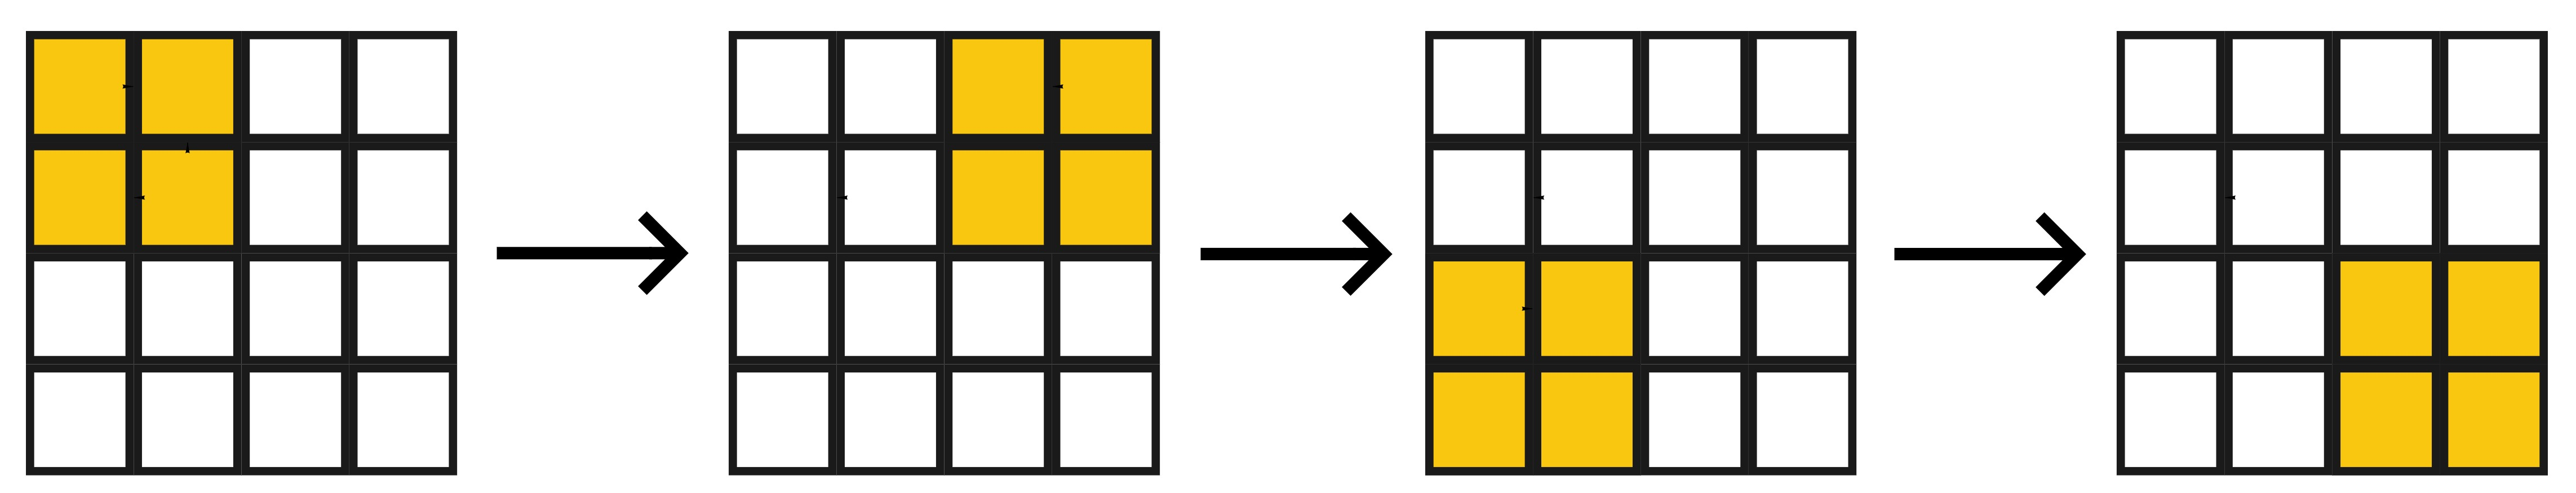
\includegraphics[width=1.0\textwidth]{imagens/conceitos_basicos/convolution_stride.jpg}
    \label{fig:convolution_stride_cnn}
    \source{Danilo Assunção, 2022}
\end{figure}

Na definição em \citeonline{yamashita2018convolutional}, o preenchimento é um método em que linhas e colunas de zeros são adicionadas em cada lado da matriz de valores que representa a imagem, de modo a ajustar o centro de um filtro no elemento mais externo, e mantendo a mesma dimensão no plano através da operação de convolução, sem o preenchimento, cada mapa de características sucessivo ficaria menor após a operação de convolução. Arquiteturas modernas para CNN geralmente empregam preenchimento zero. Na Figura \ref{fig:convolution_padding_cnn} é ilustrada a aplicação de preenchimento de 0 onde é possível observar que a imagem original e o mapa de características gerado possuem a mesma dimensão espacial.

\begin{figure}[H]
    \centering
    \caption{Exemplo do uso de preenchimento de valor 0 no processo convolucional}
    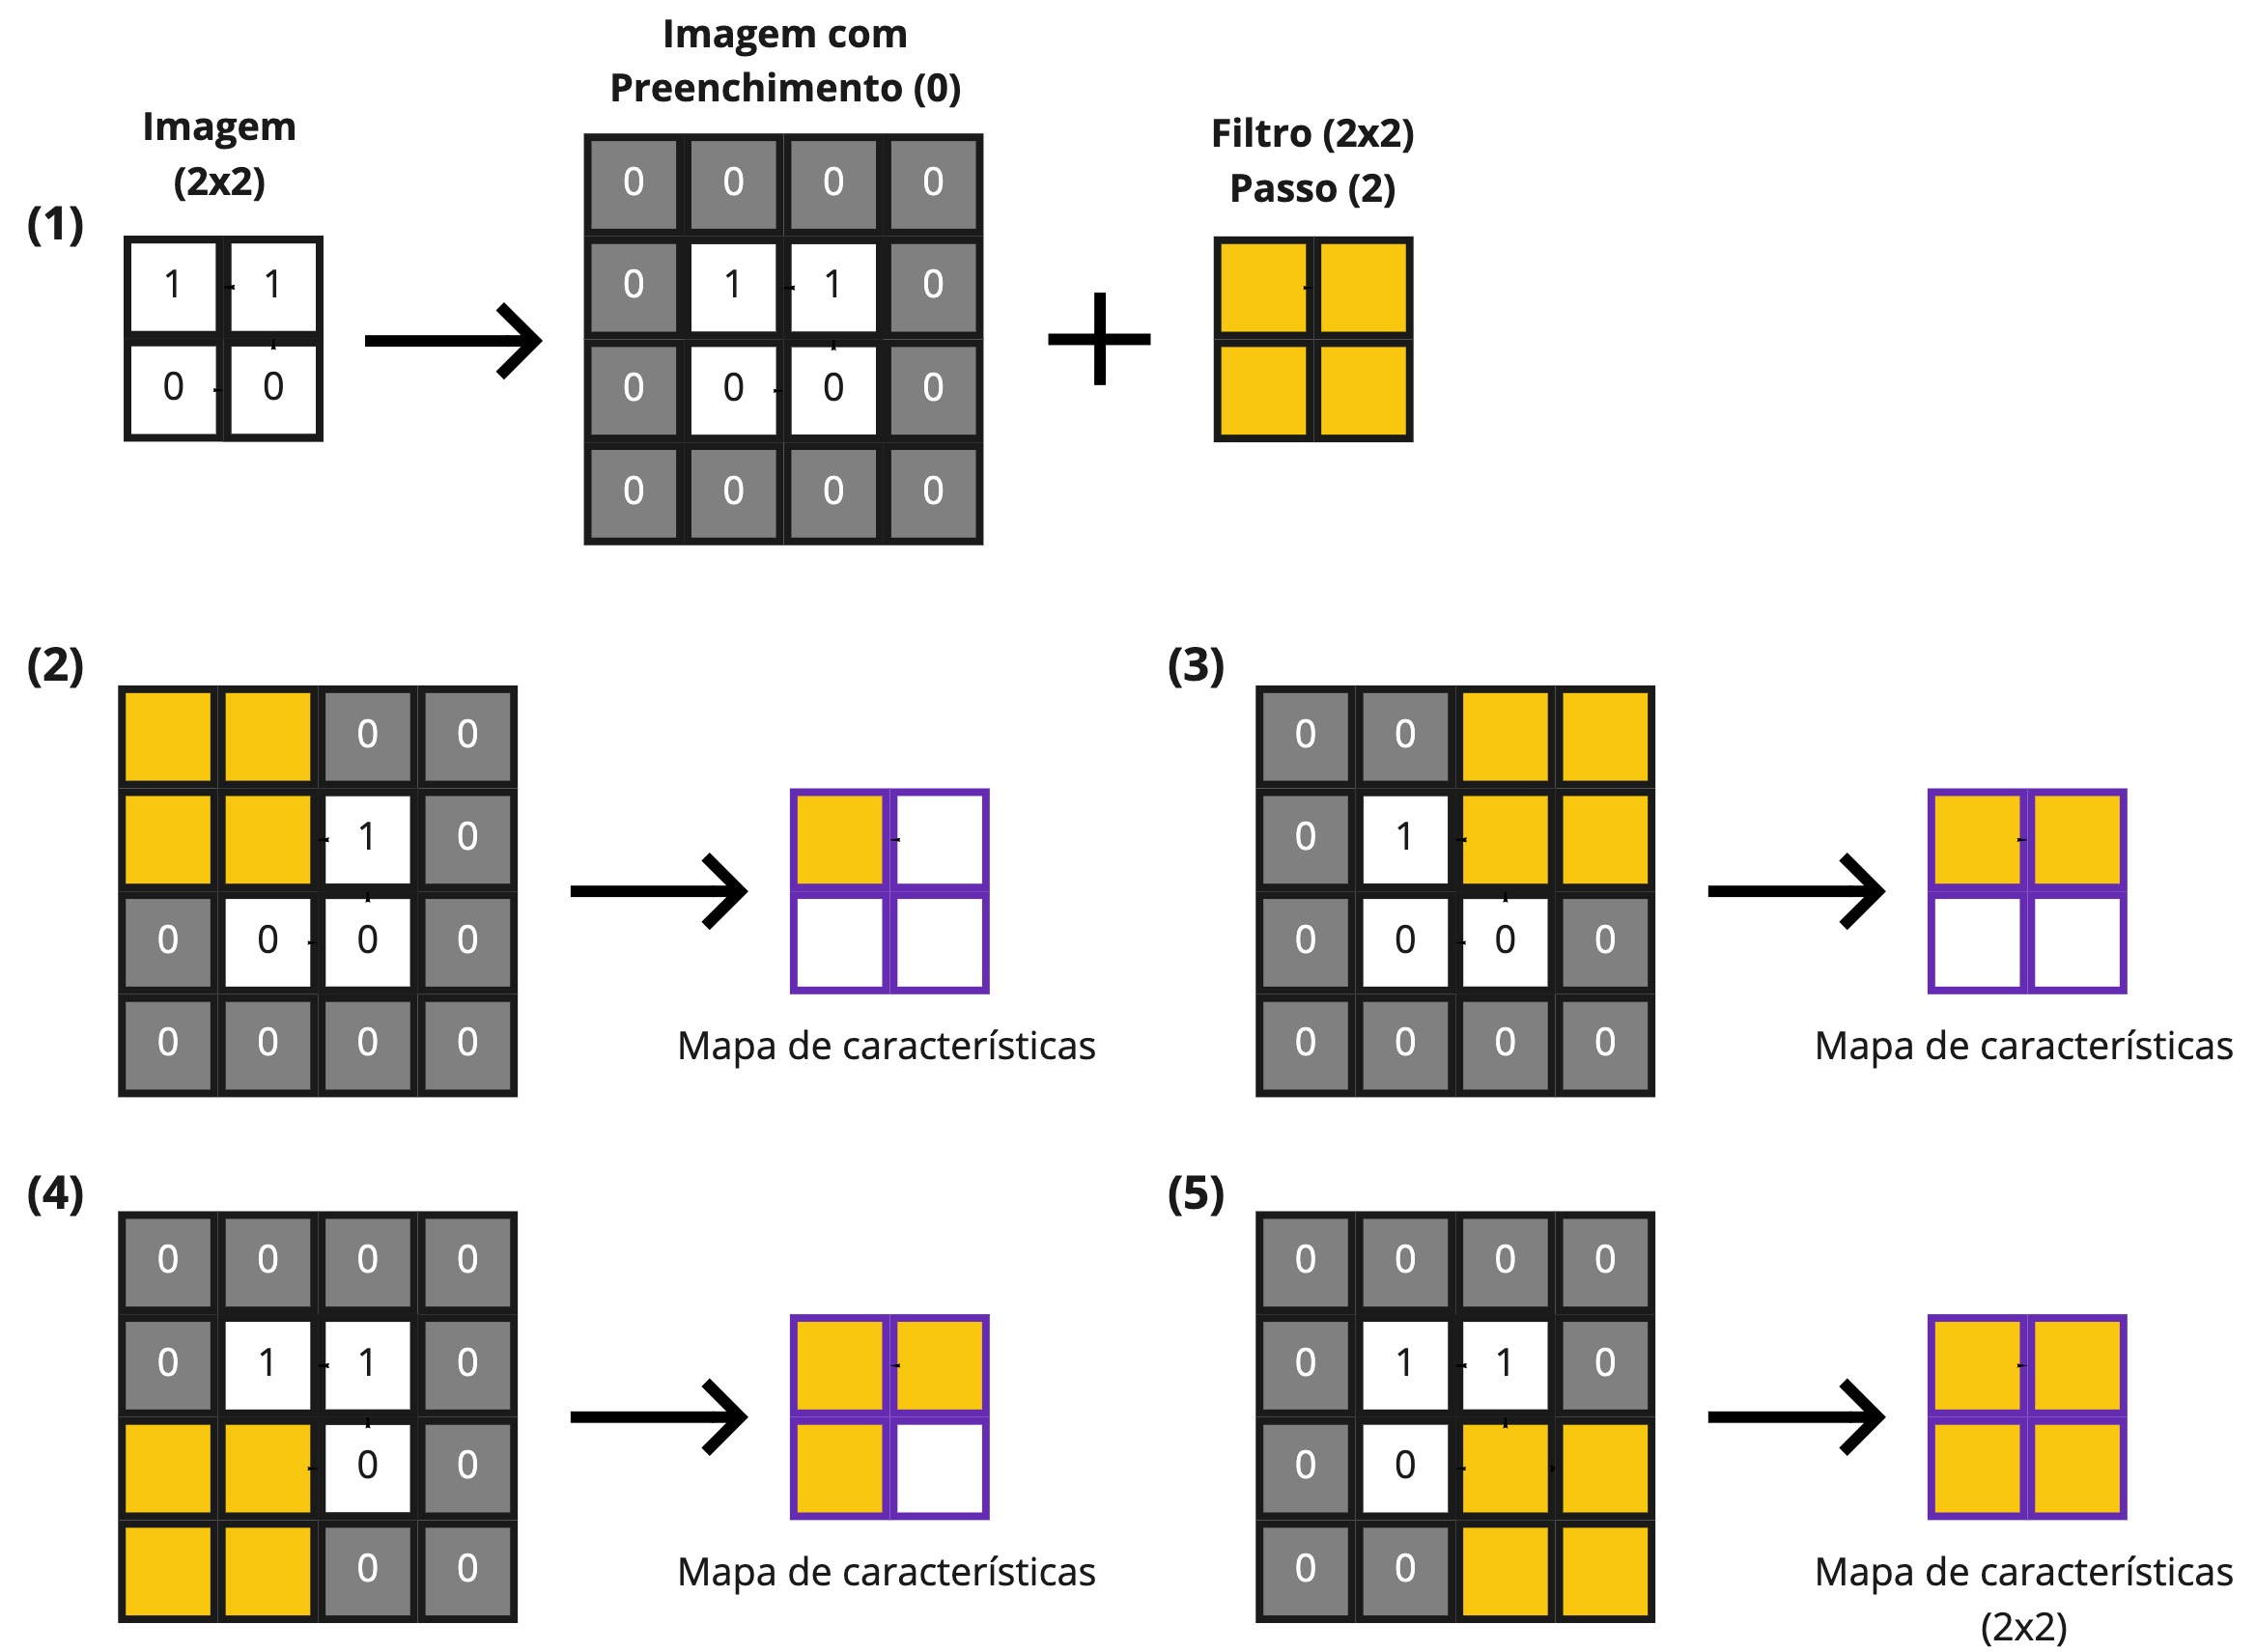
\includegraphics[width=1.0\textwidth]{imagens/conceitos_basicos/convolution_padding.jpg}
    \label{fig:convolution_padding_cnn}
    \source{Danilo Assunção, 2022}
\end{figure}

\subsection{Função de ativação não linear}
As saídas de uma operação linear, como a convolução, passam por uma função de ativação não linear. A função de ativação mais comum usada atualmente é a unidade linear retificada (ReLU), devido a facilidade em se computar suas derivadas melhorando o desempenho da rede em relação a este procedimento \cite{albawi2017understanding}. A ReLu é expressada pela Equação \ref{equation_relu}:

\begin{equation}
  ReLU(x)=\max(0, x)
  \label{equation_relu}
\end{equation}

\subsection{Camada de agrupamento}
O objetivo da camada de agrupamento (\textit{pooling layer}) é tornar a representação de características conjuntas mais utilizável, que preserve informações importantes enquanto descarta detalhes irrelevantes \cite{yu2014mixed}. Ou seja, a camada de agrupamento visa a reduzir gradualmente a dimensionalidade da representação e, assim, reduzir ainda mais o número de parâmetros e complexidade computacional do modelo \cite{o2015introduction}. A operação oferecida pelo agrupamento é tipicamente conhecida como \textit{downsampling}. É importante notar que não há nenhum parâmetro treinável nas camadas de agrupamento, enquanto o tamanho do filtro, a passada (\textit{stride}) e o preenchimento (\textit{padding}) são também hiperparâmetros em operações de agrupamento, semelhantes às operações de convolução \cite{yamashita2018convolutional}. Existem algumas funções de agrupamento presentes na literatura, abaixo será explorado o agrupamento máximo e o agrupamento médio.

Agrupamento máximo (\textit{max pooling}) é a forma mais popular de operação de agrupamento, que extrai um mapa de características condensado através do mapa de características recebido da saída da camada convolucional, obtendo apenas o valor máximo contido no mapa de características recebido e descartando os demais valores \cite{yamashita2018convolutional}. Este método pode ser observado pela Figura \ref{fig:max_pooling}.

\begin{figure}[H]
    \centering
    \caption{Agrupamento máximo}
    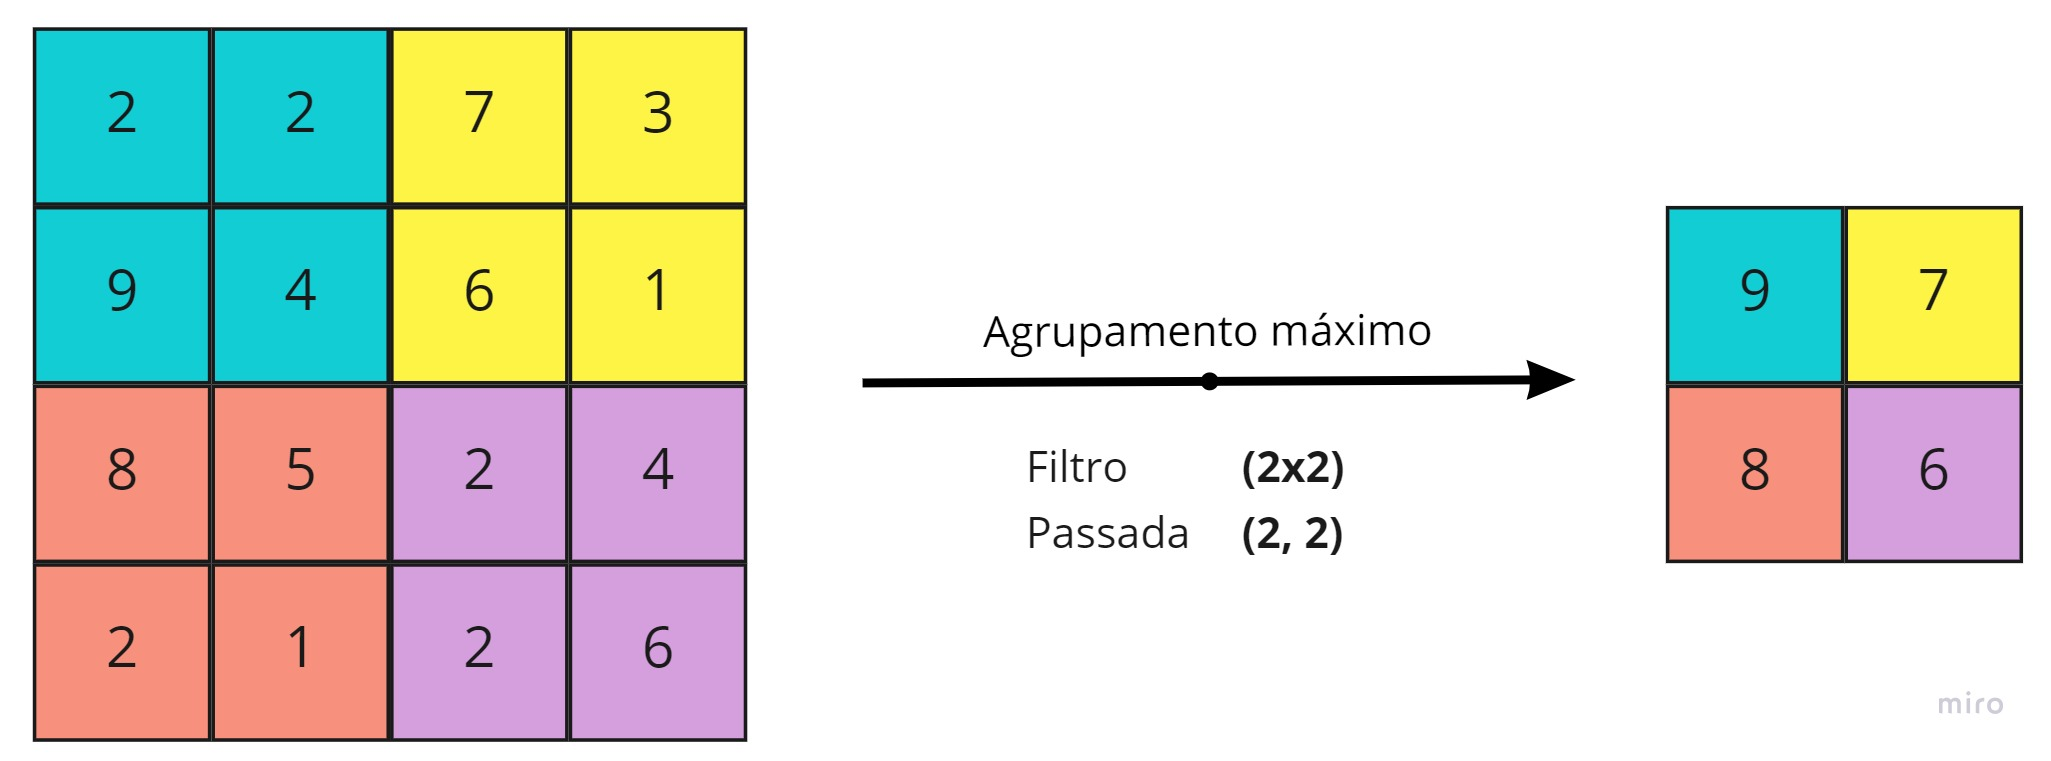
\includegraphics[width=1.0\textwidth]{imagens/conceitos_basicos/agrupamento_maximo.jpg}
    \label{fig:max_pooling}
    \source{Danilo Assunção, 2022}
\end{figure}

O agrupamento médio (\textit{average pooling}) extrai um mapa de características condensado do mapa de características recebido a partir do cálculo da média destes elementos. Assim, enquanto o agrupamento máximo fornece a característica mais proeminente em um mapa de características condensado, o agrupamento médio calcula a média dos elementos presentes na região do mapa de características coberto pelo filtro. Este método é ilustrado na Figura \ref{fig:average_pooling}.

\begin{figure}[H]
    \centering
    \caption{Agrupamento médio}
    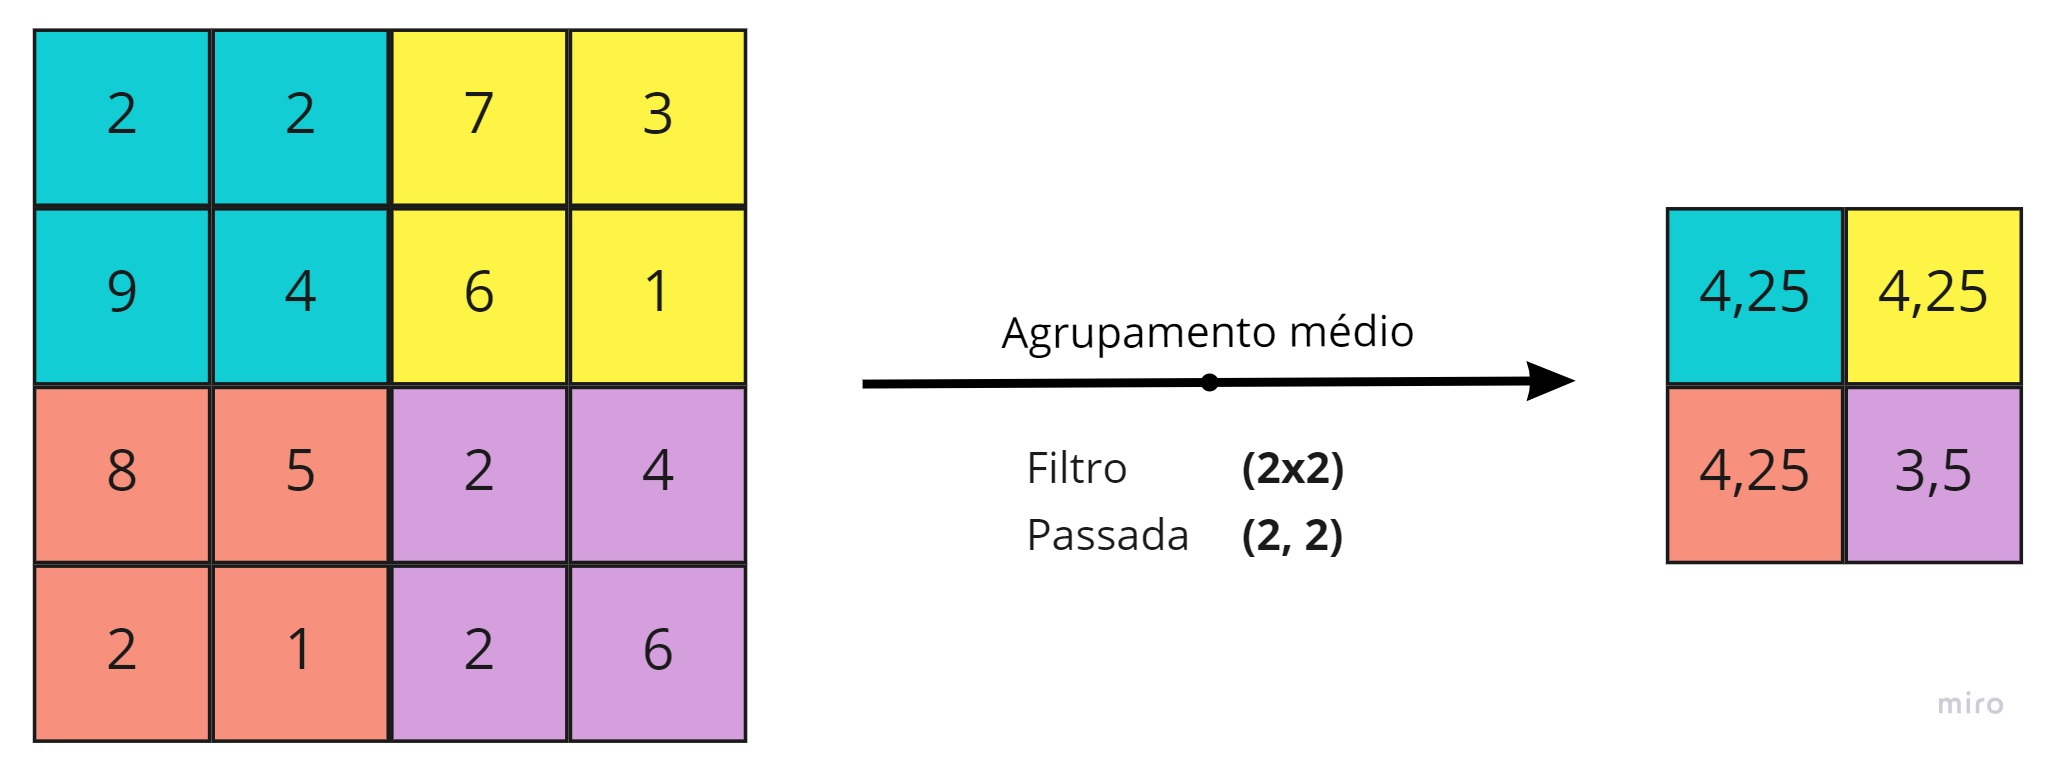
\includegraphics[width=1.0\textwidth]{imagens/conceitos_basicos/agrupamento_medio.jpg}
    \label{fig:average_pooling}
    \source{Danilo Assunção, 2022}
\end{figure}
 
\subsection{Camada totalmente conectada}
Os mapas de características de saída da convolução final ou camada de agrupamento, são normalmente achatados (\textit{flattened}), ou seja, transformados em uma matriz unidimensional (ou vetor) e conectados a uma ou mais camadas totalmente conectadas, também conhecidas como camadas densas, em que todas as entradas são conectadas a todas as saídas por um peso que se ajusta em seu procedimento de aprendizado \cite{yamashita2018convolutional}. A camada final totalmente conectada normalmente possui o mesmo número de nós de saída que o número de classes relacionadas ao domínio trabalhado no modelo \cite{yamashita2018convolutional}.

\section{Técnica de transferência de aprendizado}
A transferência de aprendizado visa a extrair o conhecimento de uma ou mais tarefas de origem e aplicar o conhecimento a uma tarefa de destino \cite{pan2009survey}. Esta técnica funciona treinando uma rede em um elevado conjunto de dados, como \textit{ImageNet} que é um grande conjunto de dados visuais projetado para uso em pesquisa de software de reconhecimento de objetos visuais \cite{russakovsky2015imagenet}, para então usar tais pesos como os pesos iniciais em uma nova tarefa de classificação. Segundo \citeonline{shao2014transfer}, a eficiência desta técnica é notada pois muitos conjuntos de dados de imagem compartilham características espaciais de baixo nível, que são melhor compreendidas a partir de um grande volume de dados. A transferência de aprendizado possui alguns métodos conhecidos na literatura, entretanto, será dado ênfase a dois métodos contextualizados nesta técnica, sendo tais métodos, a extração de características e o ajuste fino. 

Baseado na descrição em \citeonline{li2017learning}, o método de extração de características (\textit{feature extraction}) usa uma CNN pré-treinada para extrair características de uma imagem. Classificadores treinados nessas características podem alcançar resultados competitivos, às vezes superando características projetadas manualmente (\textit{handcrafted}). Este método não modifica a rede original e permite que novas tarefas se beneficiem de características complexas aprendidas em tarefas anteriores. No entanto, esses recursos não são especializados para a nova tarefa e muitas vezes podem ser aprimorados através do método ajuste fino.

O método ajuste fino (\textit{fine-tuning}) modifica os parâmetros de uma CNN pré-treinada existente para treinar em uma nova tarefa. Para isto, uma pequena taxa de aprendizado é frequentemente usada e, às vezes, parte da rede é congelada para evitar sobreajuste. Usando hiperparâmetros apropriados para treinamento, o modelo resultante geralmente supera o método de extração de características ou o aprendizado de uma rede inicializada aleatoriamente. O ajuste fino torna o processo de obtenção das características da imagem mais discriminativo para a nova tarefa, e a baixa taxa de aprendizado é um mecanismo indireto para preservar parte da estrutura representacional aprendida nas tarefas originais.

\section{Técnica de aumento de dados}
Conforme descrito em \citeonline{shorten2019survey}, a técnica de aumento de dados (\textit{data augmentation}) abrange um conjunto de métodos que aumentam o tamanho dos conjuntos de dados de treinamento, nessa conformidade, melhores modelos de aprendizado profundo podem ser construídos com eles devido a sua capacidade em minimizar o sobreajuste. A seguir são descritos alguns métodos incluídos nesta técnica que são comumente utilizados:

\begin{enumerate}
  \item \textbf{Inversão}: este método consiste em inverter o eixo horizontal ou vertical de uma imagem, em que a inversão do eixo horizontal costuma ser mais frequente do que a inversão do eixo vertical. Esta técnica é uma das mais simples de se implementar, e provou ser útil em determinados conjuntos de dados de imagens.
  
  \item \textbf{Isolamento de canais de cores}: os dados de uma imagem digital são geralmente codificados como uma matriz tridimensional (altura × largura × canais de cor). Este método inclui no isolamento de um simples canal de cor, tal como R, G ou B, sendo que a imagem pode ter sua representação de cores rapidamente convertida ao isolar um destes canais tornando os canais restantes preenchidos com valores de 0. Adicionalmente, os valores nos canais de cores da imagem (RGB) podem ser manipulados com simples operações de matriz.
  
  \item \textbf{Transformação fotométrica}: este método consiste em percorrer as imagens e diminuir ou aumentar os valores dos \textit{pixels} para uma determinada constante. Outra transformação consiste em restringir os valores dos \textit{pixels} a um determinado valor mínimo ou máximo. A representação intrínseca da cor em imagens digitais se presta a muitas estratégias de ampliação. Nesta técnica estão incluídos os métodos empregados para ajustes de iluminação da imagem ou na conversão da imagem para uma escala de cinza.
  
  \item \textbf{Corte}: cortar imagens é uma prática de processamento, em que áreas relevantes da imagem são destacadas e redimensionadas. Por exemplo, uma imagem de dimensão 256x256 em que, após o corte, ficou com dimensão 224x224. Dependendo do limite de redução escolhido para o corte, pode ser uma transformação que pode ou não preservar o tamanho original da imagem.
  
  \item \textbf{Rotação}: é a realização de rotação da imagem para a direita ou esquerda, em um eixo compreendido entre 1° e 359°. A segurança deste método é fortemente determinada pelo grau de rotação, sendo que, à medida que o grau de rotação aumenta, a classe que representa os dados pode não mais ser preservada após aplicada tal transformação.
  
  \item \textbf{Deslocamento}: é um método de deslocação de imagens para a esquerda, direita, cima ou baixo, podendo ser uma transformação muito útil para evitar um viés no modelo e preservando as dimensões da imagem. Por exemplo, se todas as imagens em um conjunto de dados estiverem centralizadas, o que é comum em conjuntos de dados de reconhecimento de rosto, exigiria que o modelo também fosse testado em imagens perfeitamente centradas. Como a imagem original foi deslocada para um direção, o espaço restante pode ser preenchido com um valor constante, no caso de um modelo na escala RGB, poderia ser aplicada a cor preta (0, 0, 0) ou a cor branca (255, 255, 255).
\end{enumerate}

\section{Conclusão}
Neste capítulo uma série de conceitos importantes foram apresentados que estão amplamente relacionados a este trabalho de pesquisa, que envolve a aplicação de Redes Neurais Convolucionais (CNNs) na resolução de problemas de reconhecimento de espécies. Contudo, as explicações para os conceitos de aprendizado de máquina e suas ramificações de mais baixo nível, como aprendizado profundo e algoritmos de CNN foram todas especificadas nesta seção, a fim de permitir um maior entendimento das definições utilizadas nos capítulos a seguir.

% ----------------------------------------------------------
% CAPITULO - REVISÃO SISTEMÁTICA
% ----------------------------------------------------------
\chapter{Revisão sistemática}
A revisão sistemática possibilita uma forma de análise e instrução a partir das informações dispostas pelos artigos disponíveis para uma pesquisa em específico, assunto de tópico ou tema de interesse, sendo que deve ser utilizada uma sistemática de confiança, auditável e integra \cite{garcia2020guidelines}.
O desenvolvimento da revisão sistemática se baseia em um protocolo devidamente definido para alcançar resultados válidos e detalhados, trazendo assim a possibilidade de análise e contradição destes resultados a partir do uso do protocolo determinado.

\section{Objetivos da revisão}
Na área de visão computacional há a aplicação de técnicas com objetivo de identificação de insetos, cuja técnica de processamento, baseado em imagens e algoritmos, acabam por reconhecer os padrões presentes nas imagens e, assim, classificar automaticamente as espécies de insetos. Tal processamento vem modificando o tradicional modelo manual e descritivo de características morfológicas já fornecido por estudos taxonômicos para a identificação destes insetos. Contudo, apenas especialistas como taxonomistas e técnicos qualificados podem identificar tais insetos com precisão, pois isso requer conhecimento especializado e obtido por meio de uma vasta experiência \cite{lim2017performance}.

O aprendizado profundo tem sido amplamente utilizado em processamento de imagens, visão computacional e reconhecimento de padrões. Diferente dos métodos tradicionais de aprendizado de máquina, o modelo de aprendizado profundo pode aprender características automaticamente a partir de uma grande quantidade de imagens, e não requer um especialista com domínio na construção do extrator de características \cite{liu2020classification}.

As características extraídas das imagens são os fatores que mais influenciam na acurácia do classificador. Embora existam várias técnicas e ferramentas para extração de características automaticamente, ainda não se encontram trabalhos na literatura que avaliem estas técnicas de aprendizado profundo e nem ferramentas que as entreguem de forma sistemática.

Portanto, o objetivo desta revisão sistemática é apresentar e discutir o estado da arte das técnicas de reconhecimento automático de espécies por meio de suas imagens e morfologias diversas, empregando técnicas de aprendizado profundo. Visando tal objetivo, foram analisados os artigos com foco na aplicação de Redes Neurais Convolucionais (CNN).

\section{Protocolo}

Foram definidas quatro fases para a realização desta revisão sistemática, sendo elas:

\begin{enumerate}
  \item Planejamento
  \item Condução
  \item Extração
  \item Consolidação
\end{enumerate}

O planejamento consiste na criação do protocolo no qual as diretrizes da pesquisa serão baseadas. A condução é a execução da pesquisa e seleção de trabalhos de interesse, de acordo com os critérios de inclusão e exclusão definidos no protocolo. A extração é a fase na qual os artigos que foram selecionados são estudados e os dados importantes são separados. Em suma, temos a consolidação, na qual os dados são cruzados para gerar conhecimento e, assim, o artigo de revisão sistemática é escrito.

Estes processos estão representados na Figura \ref{fig:processo_revisao_sistematica}, na qual cada etapa do processo está identificada com uma cor diferente.

\begin{figure}[H]
    \centering
    \caption{Diagrama do processo de revisão sistemática}
    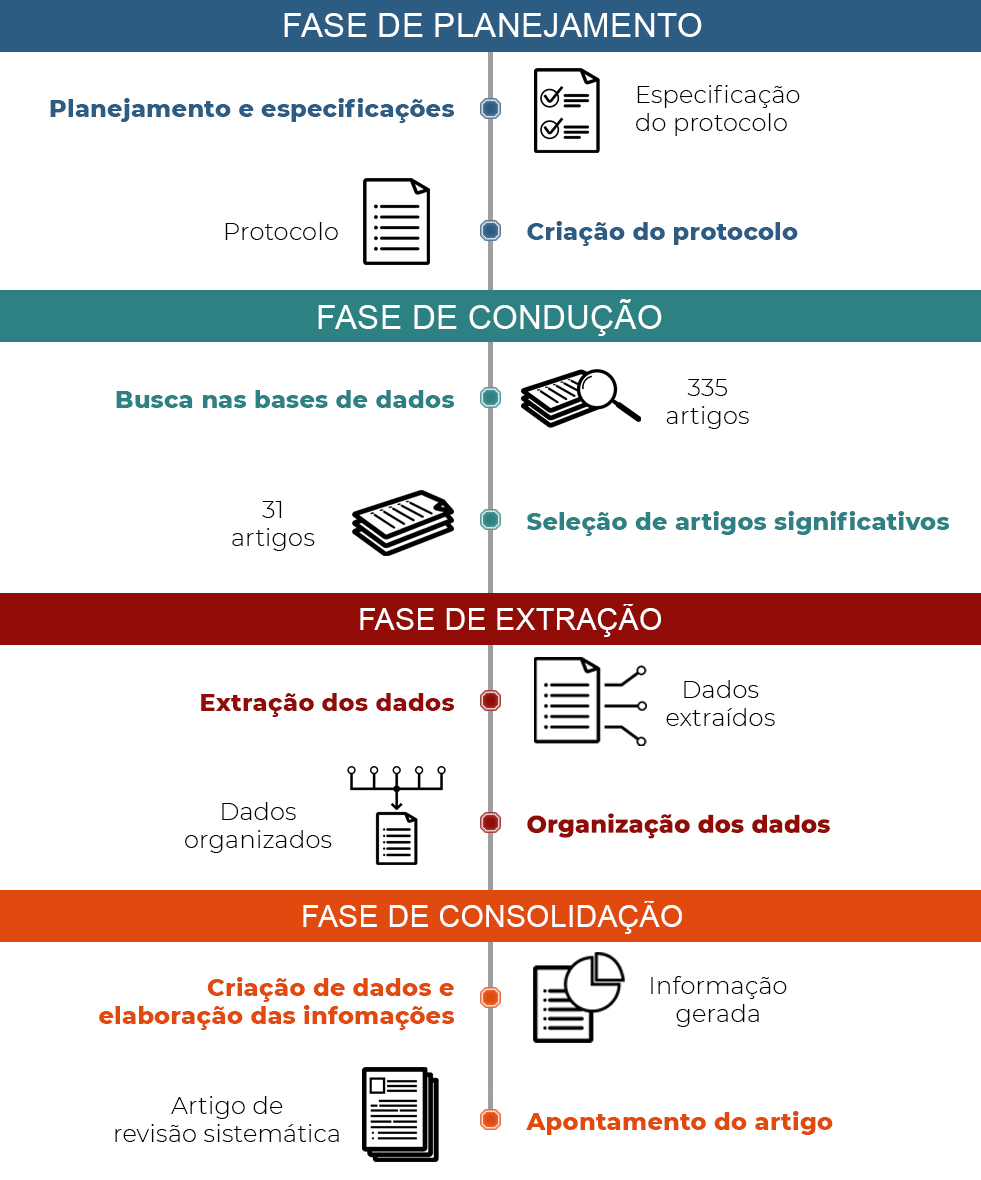
\includegraphics[scale=.35]{imagens/revisao_sistematica/processo_revisao_sistematica.jpg}
    \label{fig:processo_revisao_sistematica}
    \source{Danilo Assunção, 2021}
\end{figure}

Na etapa de planejamento foi levantada junto ao protocolo a seguinte questão:
``Quais os métodos, adeptos ao estado da arte, para a identificação de espécies de insetos usando-se uma Rede Neural Convolucional por meio de imagens digitais?''.
A conclusão desta pergunta veio a partir de bases de dados junto às seguintes \textit{strings} de busca:

\begin{itemize}
  \item \textbf{IEEE Xplore} - (``convolutional neural network'' OR ``cnn'' OR ``convolution'') AND ``feature extraction'' AND (``insect'' OR ``pest'') AND (``image'' OR ``image segmentation'' OR ``image recognition'')
  \item \textbf{SCOPUS} - (``convolutional neural network'' OR ``cnn'' OR ``convolution'') AND ``feature extraction'' AND (``insect'' OR ``pest'') AND (``image'' OR ``image segmentation'' OR ``image recognition'') AND (EXCLUDE (DOCTYPE, ``cp'') OR EXCLUDE (DOCTYPE, ``re'') OR EXCLUDE (DOCTYPE, ``bk'') OR EXCLUDE (DOCTYPE, ``ch''))
\end{itemize}

A palavra chave \textit{pest} é incluída nas \textit{strings} de busca por se tratar de um objeto de estudo muito recorrente nos meios de reconhecimento de espécies através de imagens, utilizando de técnicas similares às que são usadas para reconhecimento de insetos por meio de métodos utilizando CNN.

Este trabalho foi conduzido de dezembro de 2020 até fevereiro de 2021. Inicialmente 335 trabalhos foram encontrados nas bases de dados especificadas acima, dos quais 302 estavam na base de dados SCOPUS e 33 na base de dados IEEE Xplore.

Após aplicar os critérios de inclusão e exclusão nos trabalhos coletados, 31 artigos foram selecionados e analisados por completo, sendo 28 da base SCOPUS e 3 da base IEEE Xplore.

Os critérios utilizados para incluir ou excluir um trabalho nesta revisão foram:

\begin{itemize}
  \item Inclusão
    \begin{itemize}
        \item{Artigos que utilizam CNNs como ferramenta para discriminação de espécies por meio de imagens;}
        \item{Artigos que contêm técnicas computacionais de segmentação e extração de características de imagens de diversas espécies biológicas;}
        \item{Artigos devem ter data de publicação maior ou igual a 2015.}
    \end{itemize}
  \item Exclusão
    \begin{itemize}
        \item{Artigos que não são relacionados com conceitos envolvendo técnicas de segmentação e extração de características por meio de imagens;}
        \item{Artigos que não utilizam CNNs para classificação automática de espécies por meio de imagens;}
        \item{Artigos que não foram escritos nos idiomas inglês ou português;}
        \item{Artigos com data de publicação menor que 2015;}
        \item{Documentos que não estejam categorizados como artigo em seu tipo de documento.}
    \end{itemize}
\end{itemize}

Com a finalidade de poder encontrar possíveis lacunas nas pesquisas utilizadas, seguidamente da extração de dados, foi exercida uma averiguação sobre os principais obstáculos e propensões praticadas.

\section{Resultado da revisão sistemática}
Os 31 trabalhos selecionados foram estudados e os seguintes atributos foram extraídos: ano de publicação, técnicas de pré-processamento de imagens, técnicas de transferência de aprendizado, técnicas de aumento de dados, modelo de arquitetura da CNN e métodos de classificação. Um breve sumário dos trabalhos com os respectivos dados extraídos encontram-se no Tabela \ref{tab:sumario_artigos_selecionados}.
  
% -----------------------------------------
% TABELA - SUMÁRIO DOS ARTIGOS ANALISADOS
% -----------------------------------------
\begin{landscape}
\begin{OnehalfSpacing}
\begin{footnotesize}
\begin{longtable}{|p{2.3cm}|p{1.3cm}|p{1.8cm}|p{3cm}|p{2.4cm}|p{4.3cm}|p{4.3cm}|p{2.5cm}|}
\caption{Sumário de todos os artigos analisados} \label{tab:sumario_artigos_selecionados} \\
 
\hline \textbf{Artigo} &
  \textbf{Ano de publicação} &
  \textbf{País de afiliação dos autores} &
  \textbf{Téc. de pré-processamento de imagens} &
  \textbf{Téc. de transferência de aprendizado} &
  \textbf{Téc. de aumento de dados} &
  \textbf{Modelo de arquitetura da CNN} &
  \textbf{Modelo do classificador} \\ \hline
\endfirsthead
 
\multicolumn{8}{c}%
{{\bfseries \tablename\ \thetable{} -- continuação da página anterior}} \\
\hline \textbf{Artigo} &
  \textbf{Ano de publicação} &
  \textbf{País de afiliação dos autores} &
  \textbf{Téc. de pré- processamento de imagens} &
  \textbf{Téc. de transferência de aprendizado} &
  \textbf{Téc. de aumento de dados} &
  \textbf{Modelo de arquitetura da CNN} &
  \textbf{Modelo do classificador} \\ \hline
\endhead
 
\hline \multicolumn{8}{|r|}{{Continua na próxima página}} \\ \hline
\endfoot
 
\hline \multicolumn{8}{|c|}{Fonte - Danilo Assunção, 2021} \\ \hline
\endlastfoot
 
\cite{liu2020classification} &
  2020 &
  Estados Unidos &
  Não aplicado &
  Ajuste fino &
  \textit{Skewing}, Distorção elástica, Rotação &
  LeNet-5, AlexNet, VGGNet-16, VGGNet-19, ResNet-50, Inception v3, InceptionResNet v2 &
  Totalmente conectada \\ \hline
\cite{le2020automated} &
  2020 &
  França &
  Redimensionamento &
  Ajuste fino &
  Constante para cada canal de cor, Divisão dos canais da imagem &
  EB-Net &
  Totalmente conectada \\ \hline
\cite{zhangautomatic} &
  2020 &
  China &
  Não especificado &
  Não especificado &
  Não especificado &
  DenseNet-121 &
  Não especificado \\ \hline
\cite{liu2020grape} &
  2020 &
  China &
  Não aplicado &
  Não aplicado &
  Alto brilho, Baixo brilho, Alto contraste, Baixo contraste, Alta nitidez, Baixa nitidez, Rotação, Simetria vertical, Simetria horizontal, Ruído gaussiano, \textit{PCA Jittering} &
  DICNN &
  Totalmente conectada \\ \hline
\cite{lu2020identifying} &
  2020 &
  Taiwan &
  Redimensionamento &
  Ajuste fino &
  Inversão horizontal, Inversão vertical, Deslocamento horizontal, Deslocamento vertical, Rotação, \textit{Shearing}, Ampliação &
  VGGNet-16 &
  Totalmente conectada \\ \hline
\cite{banan2020deep} &
  2020 &
  Irã &
  Redimensionamento &
  Ajuste fino &
  Rotação, Deslocamento vertical, Deslocamento horizontal &
  VGGNet-16 &
  Totalmente conectada \\ \hline
\cite{tiwari2020comparative} &
  2020 &
  Índia &
  Não especificado &
  Não aplicado &
  Não aplicado &
  Indefinido &
  Totalmente conectada \\ \hline
\cite{li2020using} &
  2020 &
  China &
  Recorte, Redimensionamento &
  Não aplicado &
  Rotação, Recorte &
  VGGNet-16, Inception v3 &
  Totalmente conectada \\ \hline
\cite{chen2020research} &
  2020 &
  China &
  Redimensionamento &
  Ajuste fino &
  Rotação, Borrado, Oclusão &
  ResNeXt-101 &
  Totalmente conectada \\ \hline
\cite{hongclassification} &
  2020 &
  China &
  Redimensionamento, Recorte &
  Ajuste fino &
  Filtro gaussiano, Aprimoramento de contraste &
  AlexNet &
  Totalmente conectada \\ \hline
\cite{rauf2019visual} &
  2019 &
  Paquistão, Estados Unidos &
  Redimensionamento, Fundo transparente &
  Não aplicado &
  Não aplicado &
  32-Layer CNN &
  Totalmente conectada \\ \hline
\cite{gomez2019coral} &
  2019 &
  Espanha, Dinamarca &
  Não especificado &
  Ajuste fino &
  Não especificado &
  Inception v3, ResNet-50, ResNet-152, DenseNet-121, DenseNet-161 &
  Totalmente conectada \\ \hline
\cite{cibuk2019efficient} &
  2019 &
  Turquia, Estados Unidos &
  Não aplicado &
  Extração de características &
  Não aplicado &
  VGGNet-16, AlexNet &
  SVM (RBF) \\ \hline
\cite{li2019effective} &
  2019 &
  China &
  Redimensionamento &
  Não aplicado &
  Multi-scale, Rotação &
  ResNet-50 &
  Totalmente conectada \\ \hline
\cite{khalifa2019deep} &
  2019 &
  Egito, Luxemburgo &
  Não especificado &
  Não aplicado &
  Reflexão, Ampliação, Ruído gaussiano, Ruído de poisson, Efeitos de granulação, Ruído de manchas &
  Indefinido &
  Totalmente conectada \\ \hline
\cite{hsiang2019endless} &
  2019 &
  Suécia, Reino Unido &
  Redimensionamento &
  Ajuste fino &
  Não especificado &
  VGGNet-16, DenseNet-121, Inception v3 &
  Totalmente conectada \\ \hline
\cite{ren2019feature} &
  2019 &
  Japão &
  Redimensionamento, Recorte &
  Não aplicado &
  Redimensionamento, Recorte, Normalização de média e desvio padrão &
  FR-ResNet &
  Totalmente conectada \\ \hline
\cite{valan2019automated} &
  2019 &
  Suécia &
  Redimensionamento, Recorte &
  Extração de características &
  Não aplicado &
  VGGNet-16 &
  SVM (Linear) \\ \hline
\cite{gyires2019deep} &
  2019 &
  Hungria &
  Recorte, Redimensionamento &
  Ajuste fino &
  Não aplicado &
  AlexNet, Inception V3 &
  Totalmente conectada \\ \hline
\cite{thenmozhi2019crop} &
  2019 &
  Índia &
  Escala de cinza, Detecção de bordas de canny, Recorte, Redimensionamento &
  Ajuste fino &
  Reflexão, Escala, Rotação, Translation &
  VGGNet-16, VGGNet-19 &
  Totalmente conectada \\ \hline
\cite{tetila2019deep} &
  2019 &
  Brasil &
  Não especificado &
  Ajuste fino, Extração de características &
  Rotação, Escala, \textit{Scrolling}, Ampliação &
  DenseNet-201, InceptionResNet v2, ResNet-50 &
  Totalmente conectada \\ \hline
\cite{wei2018deep} &
  2018 &
  Malásia &
  Redimensionamento, Preenchimento &
  Não aplicado &
  Não aplicado &
  D-Leaf &
  Totalmente conectada \\ \hline
\cite{zhu2018method} &
  2018 &
  China &
  Não especificado &
  Não aplicado &
  Não aplicado &
  Inception v2 &
  Totalmente conectada \\ \hline
\cite{zhu2018plant} &
  2018 &
  China &
  Redimensionamento &
  Não especificado &
  Não aplicado &
  Indefinido &
  SVM (Linear) \\ \hline
\cite{villon2018deep} &
  2018 &
  França &
  Não especificado &
  Não aplicado &
  Não aplicado &
  GoogLeNet &
  Totalmente conectada \\ \hline
\cite{lee2017deep} &
  2017 &
  Malásia, Reino Unido &
  Redimensionamento &
  Ajuste fino &
  Rotação &
  Indefinido &
  Totalmente conectada \\ \hline
\cite{zielinski2017deep} &
  2017 &
  Polônia &
  Não especificado &
  Extração de características &
  Não aplicado &
  AlexNet, VGGNet-M, VGGNet-VD &
  SVM (Linear, RBF e Polinomial), Floresta aleatória \\ \hline
\cite{wang2017crop} &
  2017 &
  China &
  Não especificado &
  Não especificado &
  Não aplicado &
  LeNet-5, AlexNet &
  Totalmente conectada \\ \hline
\cite{lim2017performance} &
  2017 &
  Coreia do Sul &
  Redimensionamento, Recorte &
  Não especificado &
  Rotação, Ampliação &
  AlexNet &
  Totalmente conectada \\ \hline
\cite{sun2017deep} &
  2017 &
  China &
  Não especificado &
  Não aplicado &
  Não aplicado &
  ResNet-26 &
  Totalmente conectada \\ \hline
 
\end{longtable}
\end{footnotesize}
\end{OnehalfSpacing}
\end{landscape}

\subsection{Ano de publicação}
Nesta revisão sistemática foi coletado o ano de publicação dos artigos, dessa maneira, fez-se  uma análise de tendência referente aos assuntos que abordam técnicas de reconhecimento de espécies utilizando uma CNN, em domínios que envolvem assuntos relacionados ao reconhecimento de espécies.

Visando a uma melhor compreensão sobre a quantidade de publicações com base em assuntos que envolvem reconhecimento automático de espécies utilizando técnicas de aprendizado profundo, foi elaborado um gráfico com todos os artigos encontrados na base de dados pela consulta feita nas bases do SCOPUS e IEEE Xplore. 

Na Figura \ref{fig:grafico_ano_vs_quantidade} é apresentado uma linha de tendência aos assuntos envolvendo os artigos encontrados pela \textit{string} de busca que possuem as palavras chaves relacionadas com, aprendizado profundo, CNNs e reconhecimento de espécies.

\begin{figure}[H]
    \centering
    \caption{Ano de publicação dos artigos com base em palavras chaves}
    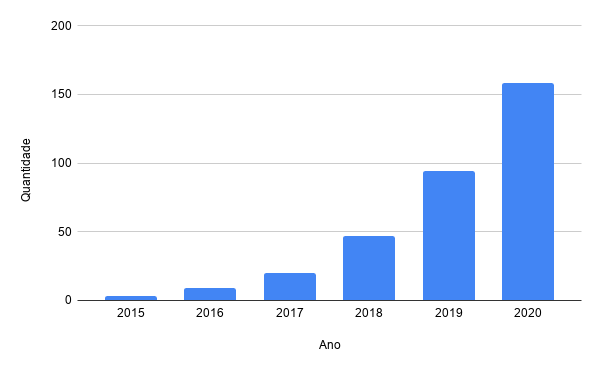
\includegraphics[width=1.0\textwidth]{imagens/revisao_sistematica/grafico_ano_vs_quantidade.png}
    \label{fig:grafico_ano_vs_quantidade}
    \source{Danilo Assunção, 2021}
\end{figure}

Na Figura \ref{fig:grafico_ano_vs_publicacao} é apresentada uma relação de quantidade versus ano, para o total de artigos que foram filtrados e selecionados a partir do conjunto obtido nas consultas executadas nas bases do SCOPUS e IEEE Xplore para esta revisão sistemática.

\begin{figure}[H]
    \centering
    \caption{Ano de publicação dos artigos selecionados}
    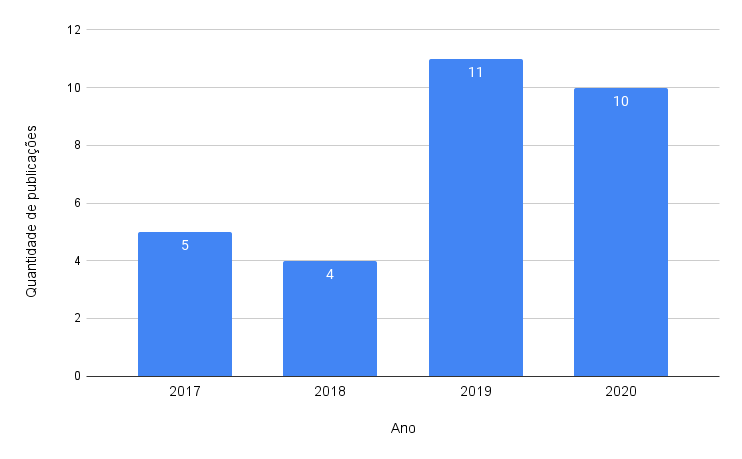
\includegraphics[width=1.0\textwidth]{imagens/revisao_sistematica/grafico_ano_vs_publicacao.png}
    \label{fig:grafico_ano_vs_publicacao}
    \source{Danilo Assunção, 2021}
\end{figure}

Nota-se que a maior quantidade dos artigos selecionados foi publicada em 2019, representando um total de 36,67\% (11). Já em 2020, é tido 33,33\% (10) dos artigos. Em 2018 a quantidade de artigos foi de 13,33\% (4) e em 2017, 16,67\% (5).

É possível perceber que, desde 2017 até 2020, houve um aumento significativo de artigos de interesse publicados com relação à aplicação de CNNs que almejam a resolução de problemas envolvendo reconhecimento de espécies em imagens digitais. Essa representatividade indica a veracidade de uma tendência de alta, com relação à utilização de técnicas envolvendo CNNs neste tipo de aplicação \cite{liu2020classification}.

Os artigos de interesse obtidos possuem data de publicação a partir do ano de 2017, os artigos de 2015 a 2016 não se mostraram muito relevantes para os assuntos relacionados à esta revisão sistemática, sendo levado em consideração os critérios de exclusão definidos.

\subsection{Técnicas de pré-processamento de imagens}
Nos métodos abordados nos artigos selecionados é possível identificar a utilização de técnicas de pré-processamento de imagens em alguns cenários distintos como é apresentado na Figura \ref{fig:grafico_preprocessamento_vs_uso}.

\begin{figure}[H]
    \centering
    \caption{Técnicas de pré-processamento de imagens aplicadas}
    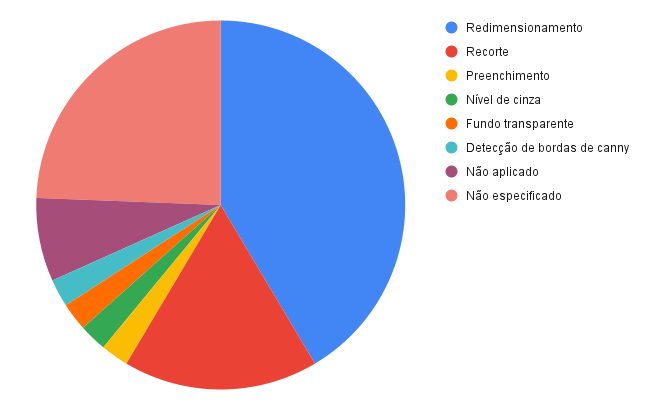
\includegraphics[width=1.0\textwidth]{imagens/revisao_sistematica/grafico_preprocessamento_vs_uso.png}
    \label{fig:grafico_preprocessamento_vs_uso}
    \source{Danilo Assunção, 2021}
\end{figure}

O papel da técnica de pré-processamento, em cenários de classificação por meio de imagens, é um processo importante, pois ele permite destacar as características importantes que podem vir a melhorar o desempenho do classificador \cite{thenmozhi2019crop}. A técnica de Redimensionamento lidera com 41,46\% de uso com relação às outras estratégias abordadas, e isso se deve aos fatores que auxiliam no aumento do desempenho do classificador, como a quantidade reduzida de parâmetros dado que a imagem é normalmente reduzida. Em segundo, com 17,07\%, o Recorte que pode vir a ser utilizado para destacar a região de interesse da imagem e reduzindo também o tamanho da imagem \cite{thenmozhi2019crop}. Preenchimento, Nível de cinza, Fundo transparente e Detecção de bordas de canny foram algumas das abordagens utilizadas, e ocupam apenas 2,44\% de uso com relação aos outros métodos. Já os 31,71\% restantes, são artigos que não aplicam ou não especificam diretamente o uso de técnicas de pré-processamento de imagens, e isto pode ser ocasionado pelo fato do conjunto de dados utilizado já estar previamente pré-processado em sua disponibilização, ou de não haver a necessidade direta de uma preparação de tais dados.

\subsection{Técnica de transferência de aprendizado}
Dois métodos foram comumente utilizados como técnicas de transferência de aprendizado, sendo elas, o método ajuste fino e o método extração de características, já em outros trabalhos o método não foi aplicado ou não foi especificado algo relacionado a isso. A Figura \ref{fig:grafico_transfer-learning_vs_uso} ilustra os dados coletados por meio dos artigos analisados que utilizam de técnicas de transferência de aprendizado, na resolução de cenários que abordam o uso de CNNs.

\begin{figure}[H]
    \centering
    \caption{Técnicas de Transferência de aprendizado}
    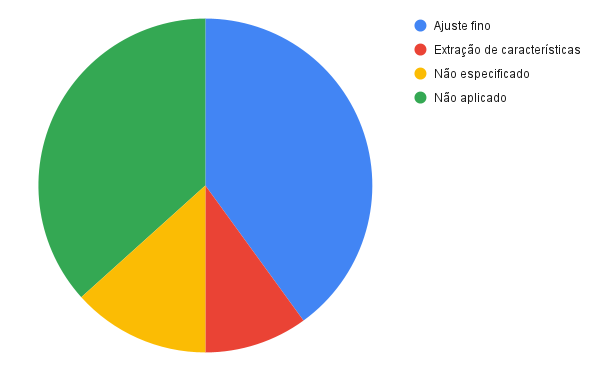
\includegraphics[width=1.0\textwidth]{imagens/revisao_sistematica/grafico_transfer_learning_vs_uso.png}
    \label{fig:grafico_transfer-learning_vs_uso}
    \source{Danilo Assunção, 2021}
\end{figure}

O ajuste fino foi o método mais utilizado com 40\% (12) de uso em relação a todas as outras técnicas encontradas nos artigos analisados. Isso revela os aspectos positivos ao se utilizar o método de ajuste fino com CNN pré-treinadas para novas tarefas \cite{li2017learning}, dado que isso auxiliou em diversos trabalhos que compõem este percentual de utilização. O uso do método de extração de características teve uso em apenas 10\% (3) dos trabalhadas analisados, e este baixo uso também pode implicar que o uso do ajuste fino é normalmente mais comum dado que o ajuste fino pode apresentar dependendo do domínio resultados melhores \cite{li2017learning}. Já nos demais trabalhos analisados, um total de 36,67\% (11) não utilizaram esta técnica e 13,33\% (4) não especificaram diretamente se houve ou não o uso da técnica de transferência de aprendizado.

\subsection{Técnicas de aumento de dados}
O método de aumento de dados permite aumentar artificialmente o tamanho do conjunto de treinamento. O aumento do conjunto de treinamento é feito ao aplicar várias distorções às imagens originais, como zoom, virando-as horizontalmente ou verticalmente, girando-as, deslocando-as e dentre outros \cite{gomez2019coral}. Na Figura \ref{fig:grafico_aumento-dados_vs_uso} são apresentados graficamente os métodos utilizados para o aumento de dados nos artigos abordados.

\begin{figure}[H]
    \centering
    \caption{Métodos para o aumento de dados}
    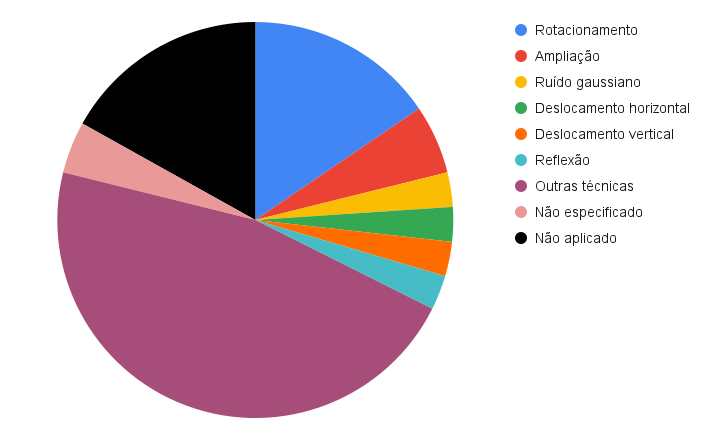
\includegraphics[width=1.0\textwidth]{imagens/revisao_sistematica/grafico_aumento_dados_vs_uso.png}
    \label{fig:grafico_aumento-dados_vs_uso}
    \source{Danilo Assunção, 2021}
\end{figure}

As técnicas de Aumento de dados utilizando Rotacionamento são bem prioritárias quando este mecanismo é aplicado, com um total de uso de 15,49\% (11) com relação aos outros meios. Ampliação, sendo a terceira metodologia mais aplicada com 5,63\% (4). Ruído gaussiano, Deslocamento horizontal, Deslocamento vertical e Reflexão representando 2,82\% (2) nos demais cenários. As Outras técnicas agrupadas são métodos que foram vistos sendo utilizados somente uma única vez nos artigos selecionados e o conjunto não especificado são aos artigos que não esclarecem de maneira explícita o tipo de técnica de Aumento de dados utilizada. Entretanto, a maioria dos artigos não aplicou técnicas de Aumento de dados, com uma representação de 16,90\% (12) de todos os exemplares analisados, isto pode ser ocasionado pelo fato dos conjuntos de dados utilizados pelos autores já serem grandes o suficiente.

\subsection{Modelo de arquitetura da CNN}
É possível identificar na literatura uma grande quantidade de arquiteturas de CNNs sendo utilizadas em diversas soluções de problemas que envolvem a classificação morfológica de espécies, por meio de suas imagens digitais. Na Figura \ref{fig:grafico_arquitetura_vs_uso} é possível observar graficamente estes dados.

\begin{figure}[H]
    \centering
    \caption{Arquitetura de CNNs}
    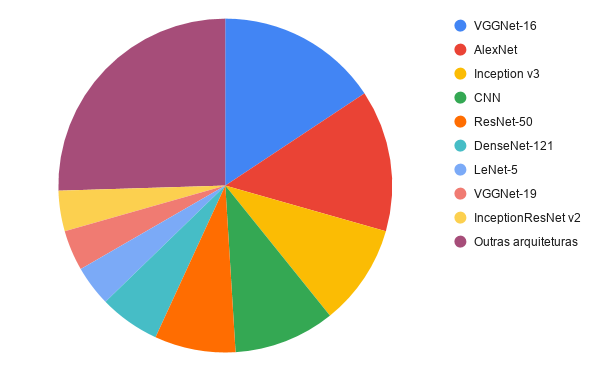
\includegraphics[width=1.0\textwidth]{imagens/revisao_sistematica/grafico_arquitetura_vs_uso.png}
    \label{fig:grafico_arquitetura_vs_uso}
    \source{Danilo Assunção, 2021}
\end{figure}

A VGGNet-16 (VGG16) foi usada em 14,29\% (8) dos trabalhos pesquisados, dado que as arquiteturas de VGG possuem maiores profundidades com filtros convolucionais menores, podendo assim reduzir os parâmetros a serem computados, além disso, as arquiteturas VGG costumam ter bons resultados \cite{li2020using}. Enquanto a AlexNet, foi aplicada em 12,50\% (7) dos casos pesquisados. As arquiteturas Inception v3 e Indefinido, em que a categoria Indefinido neste contexto representa as arquiteturas implementadas pelos autores em seus artigos, representam 7,81\% (5) de aplicações nos artigos selecionados nesta revisão sistemática, enquanto a ResNet-50 apresenta somente 6,25\% (4) e DenseNet-121 com 4,69\% (3). Já a LeNet-5, VGGNet-19 (VGG19) e InceptionResNet v2 se encontram com 3,13\% (2) de aplicabilidade. Enquanto as ``Outras arquiteturas'' que compõem 20,31\% do restante das arquiteturas utilizadas, possuem uma única utilização em seus respectivos artigos.

Para uma diferente perspectiva de visualização de usabilidade das arquiteturas de CNNs extraídas nos trabalhos em questão, foi feito um agrupamento por tipo de arquitetura para a identificação dos exemplares mais utilizados, como é mostrado na Figura \ref{fig:grafico_arquitetura_agrupada_vs_uso}.

\begin{figure}[H]
    \centering
    \caption{Tipos agrupados de arquiteturas de CNNs}
    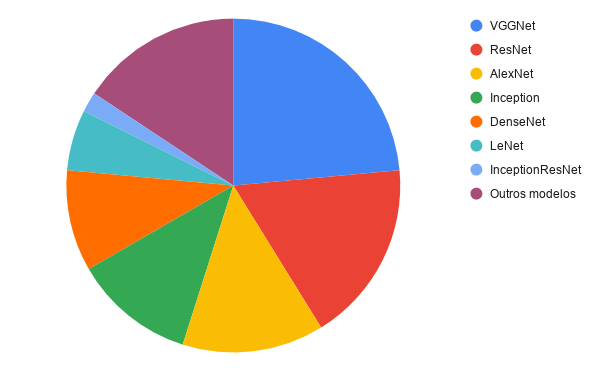
\includegraphics[width=1.0\textwidth]{imagens/revisao_sistematica/grafico_arquitetura_agrupada_vs_uso.png}
    \label{fig:grafico_arquitetura_agrupada_vs_uso}
    \source{Danilo Assunção, 2021}
\end{figure}

Nota-se que modelos de VGGNet com uso de 23,53\% (12) ainda dominam em termos de arquiteturas aplicadas na resolução de problemas envolvendo a identificação de espécies. Arquiteturas do tipo ResNet ocupam o segundo lugar com 17,65\% (9), isso devido ao seu comportamento de aumentar a profundidade da rede, sendo assim, as ResNets oferecem melhores recursos de aproximação de função (convergência ao resultado) à medida em que ganham mais parâmetros, contribuindo com sucesso na resolução de problemas como os de dissipação de gradiente, em que alguns modelos mais tradicionais acabam não conseguindo solucioná-lo, tendo resultados inferiores ao desejado \cite{sun2017deep}. Tendo a AlexNet em terceiro com 13,73\% (7), sendo este tipo de arquitetura um modelo pré-treinado de rede neural convolucional que permite a aplicação de transferência de aprendizado para que atinja melhores resultados \cite{hongclassification}. Modelos de Inception 11,76\% (6), DenseNet 9,80\% (5), LeNet 5,88\% (5) e InceptionResNet 1,96\% (1) são as arquiteturas que menos apareceram nos trabalhos avaliados. Por último, os ``Outros modelos'' que são arquiteturas de CNN desenvolvidas pelos autores dos artigos com especificidade para solucionar os seus respectivos problemas abordados.

\subsection{Métodos de classificação}
Nos trabalhos analisados é possível determinar a usabilidade de alguns tipos de algoritmos para classificação dos modelos nestes trabalhos. Dessa forma, a Figura \ref{fig:grafico_classificador_vs_uso} apresenta os exemplares aplicados nos artigos em questão.

\begin{figure}[H]
    \centering
    \caption{Método de classificação utilizado}
    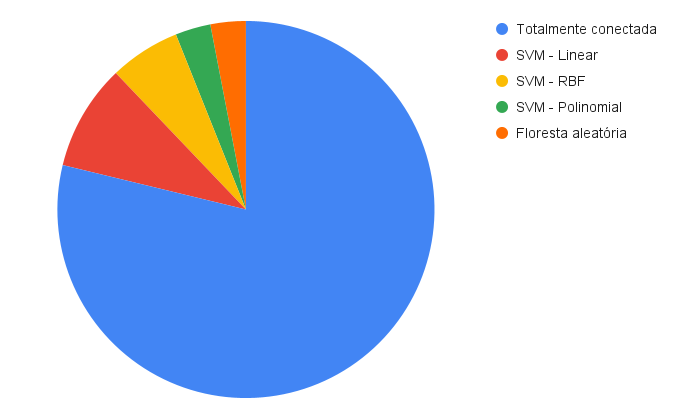
\includegraphics[width=1.0\textwidth]{imagens/revisao_sistematica/grafico_classificador_vs_uso.png}
    \label{fig:grafico_classificador_vs_uso}
    \source{Danilo Assunção, 2021}
\end{figure}

A maioria das pesquisas analisadas utilizam redes totalmente conectadas, isto é, 78,79\% (26) dos trabalhos e de fato tal presença deste método condiz com o padrão comumente visto na camada totalmente conectada de uma CNN. Nos demais cenários, onde a CNN é utilizada somente para extração de características, é tido a aplicação conjunta com alguns métodos (algoritmos) de classificação, sendo eles, SVM com \textit{kernel} Linear 9,09\% (3), RBF (função de base radial) 6,06\% (2), Polinomial 3,03\% (1) e Floresta aleatória 3,03\% (1).

\section{Conclusão}
Após o término da revisão sistemática é perceptível que o uso de técnicas de aprendizado profundo, como CNNs, vem sendo empregadas em diversos cenários em que há a necessidade de otimização no processo de extração de características das imagens, para assim, solucionar problemas que envolvem reconhecimento de espécies. Um dos atributos mais importantes é a sua capacidade de aprender as características de mais alto nível de uma imagem, e fornecer prontamente uma quantidade de informações relevantes que permitam que os algoritmos de classificação possam identificar com mais eficácia o objeto visualizado. Entretanto, é importante ressaltar que o uso deste mecanismo exige uma quantidade muito grande de dados, justamente para que seu resultado venha a convergir para um modelo que tenha a capacidade de efetivar tal atividade, e para isto foi observado na literatura o uso de técnicas como transferência de aprendizado e aumento de dados que permitem a utilização de CNNs, mesmo com um conjunto pequeno de dados disponíveis e demonstrando também que o uso de pré-processamento ainda pode vir a ser extremamente útil em cenários diversos envolvendo processamento de imagens digitais.

%------------------------------------------------------------------------
% CAPITULO - Materiais e métodos
%------------------------------------------------------------------------
\chapter{Materiais e métodos}
Visando a atingir o objetivo desta pesquisa, serão conduzidos experimentos com base em um conjunto de dados de treinamento, validação e teste utilizando uma arquitetura de CNN em união com técnicas de aumento de dados e transferência de aprendizado para aprimoramento dos resultados visados em cima do problema abordado. No conjunto de dados de treinamento, validação e teste, serão utilizadas as imagens de asas de abelhas obtidas em um ângulo que mostre a face da asa, de tal maneira a expor claramente suas nervuras, tal exemplo de uma instância deste conjunto de dados pode ser observado na Figura \ref{fig:02_mel_trigona_spinipes}. As imagens contidas nos conjuntos de dados já foram previamente rotuladas com a espécie da abelha por um especialista da área.

\begin{figure}[H]
    \centering
    \caption{Asa de abelha da espécie \textit{Trigona spinipes}}
    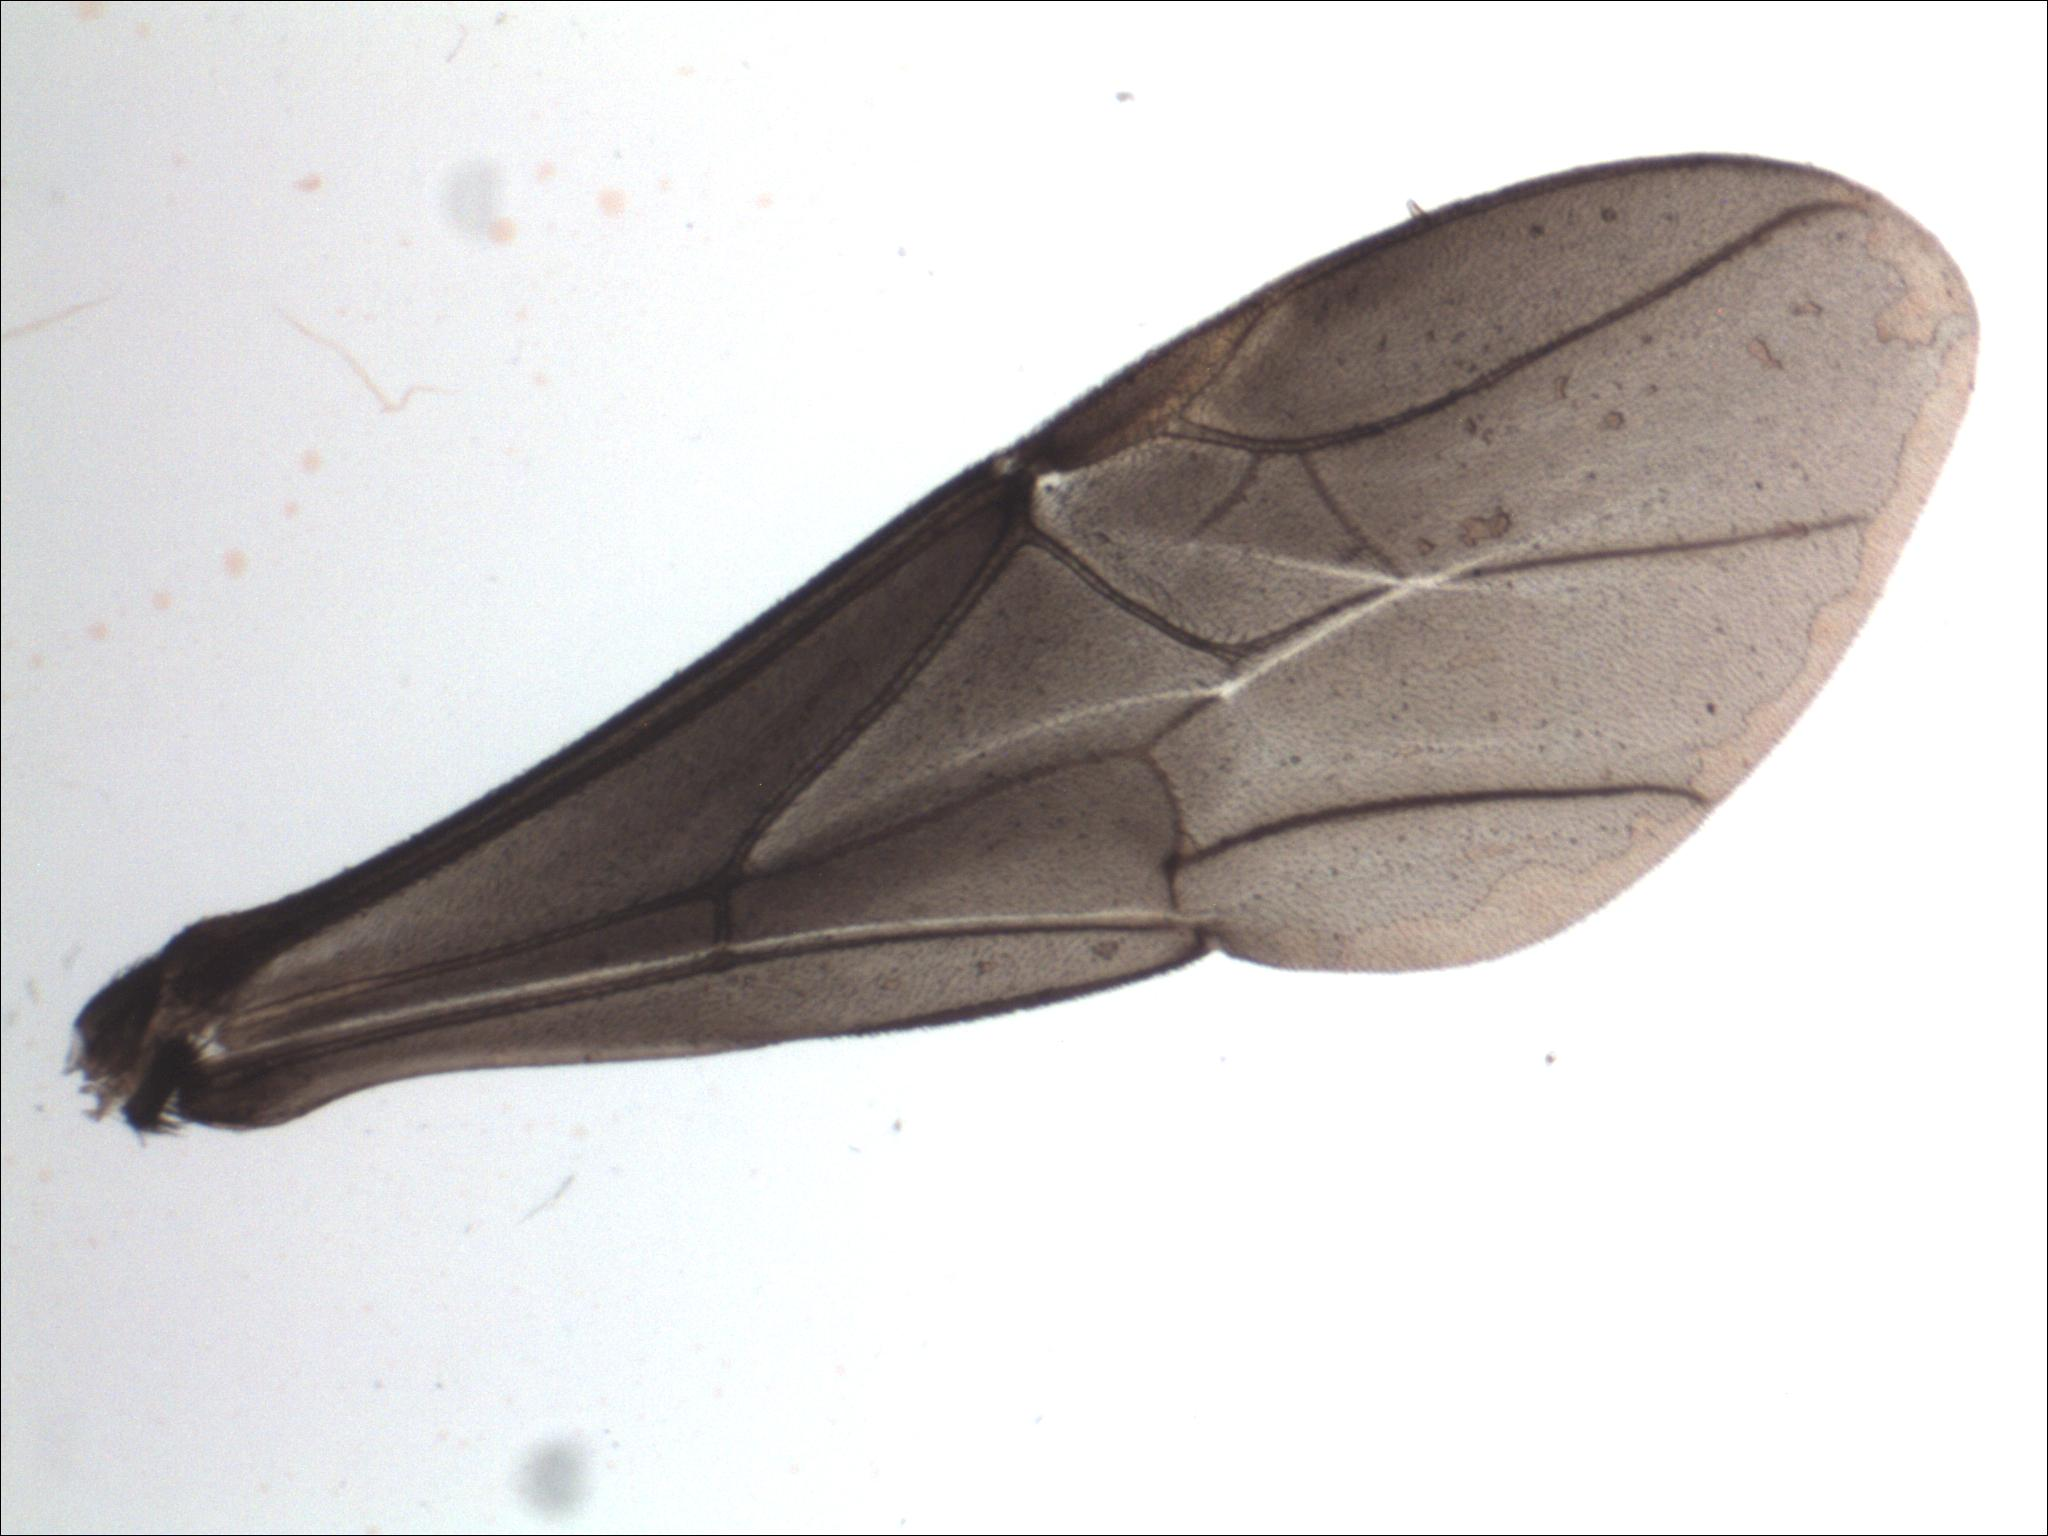
\includegraphics[width=.45\textwidth]{imagens/materiais_metodos/02_mel_trigona_spinipes.jpg}\hfill
    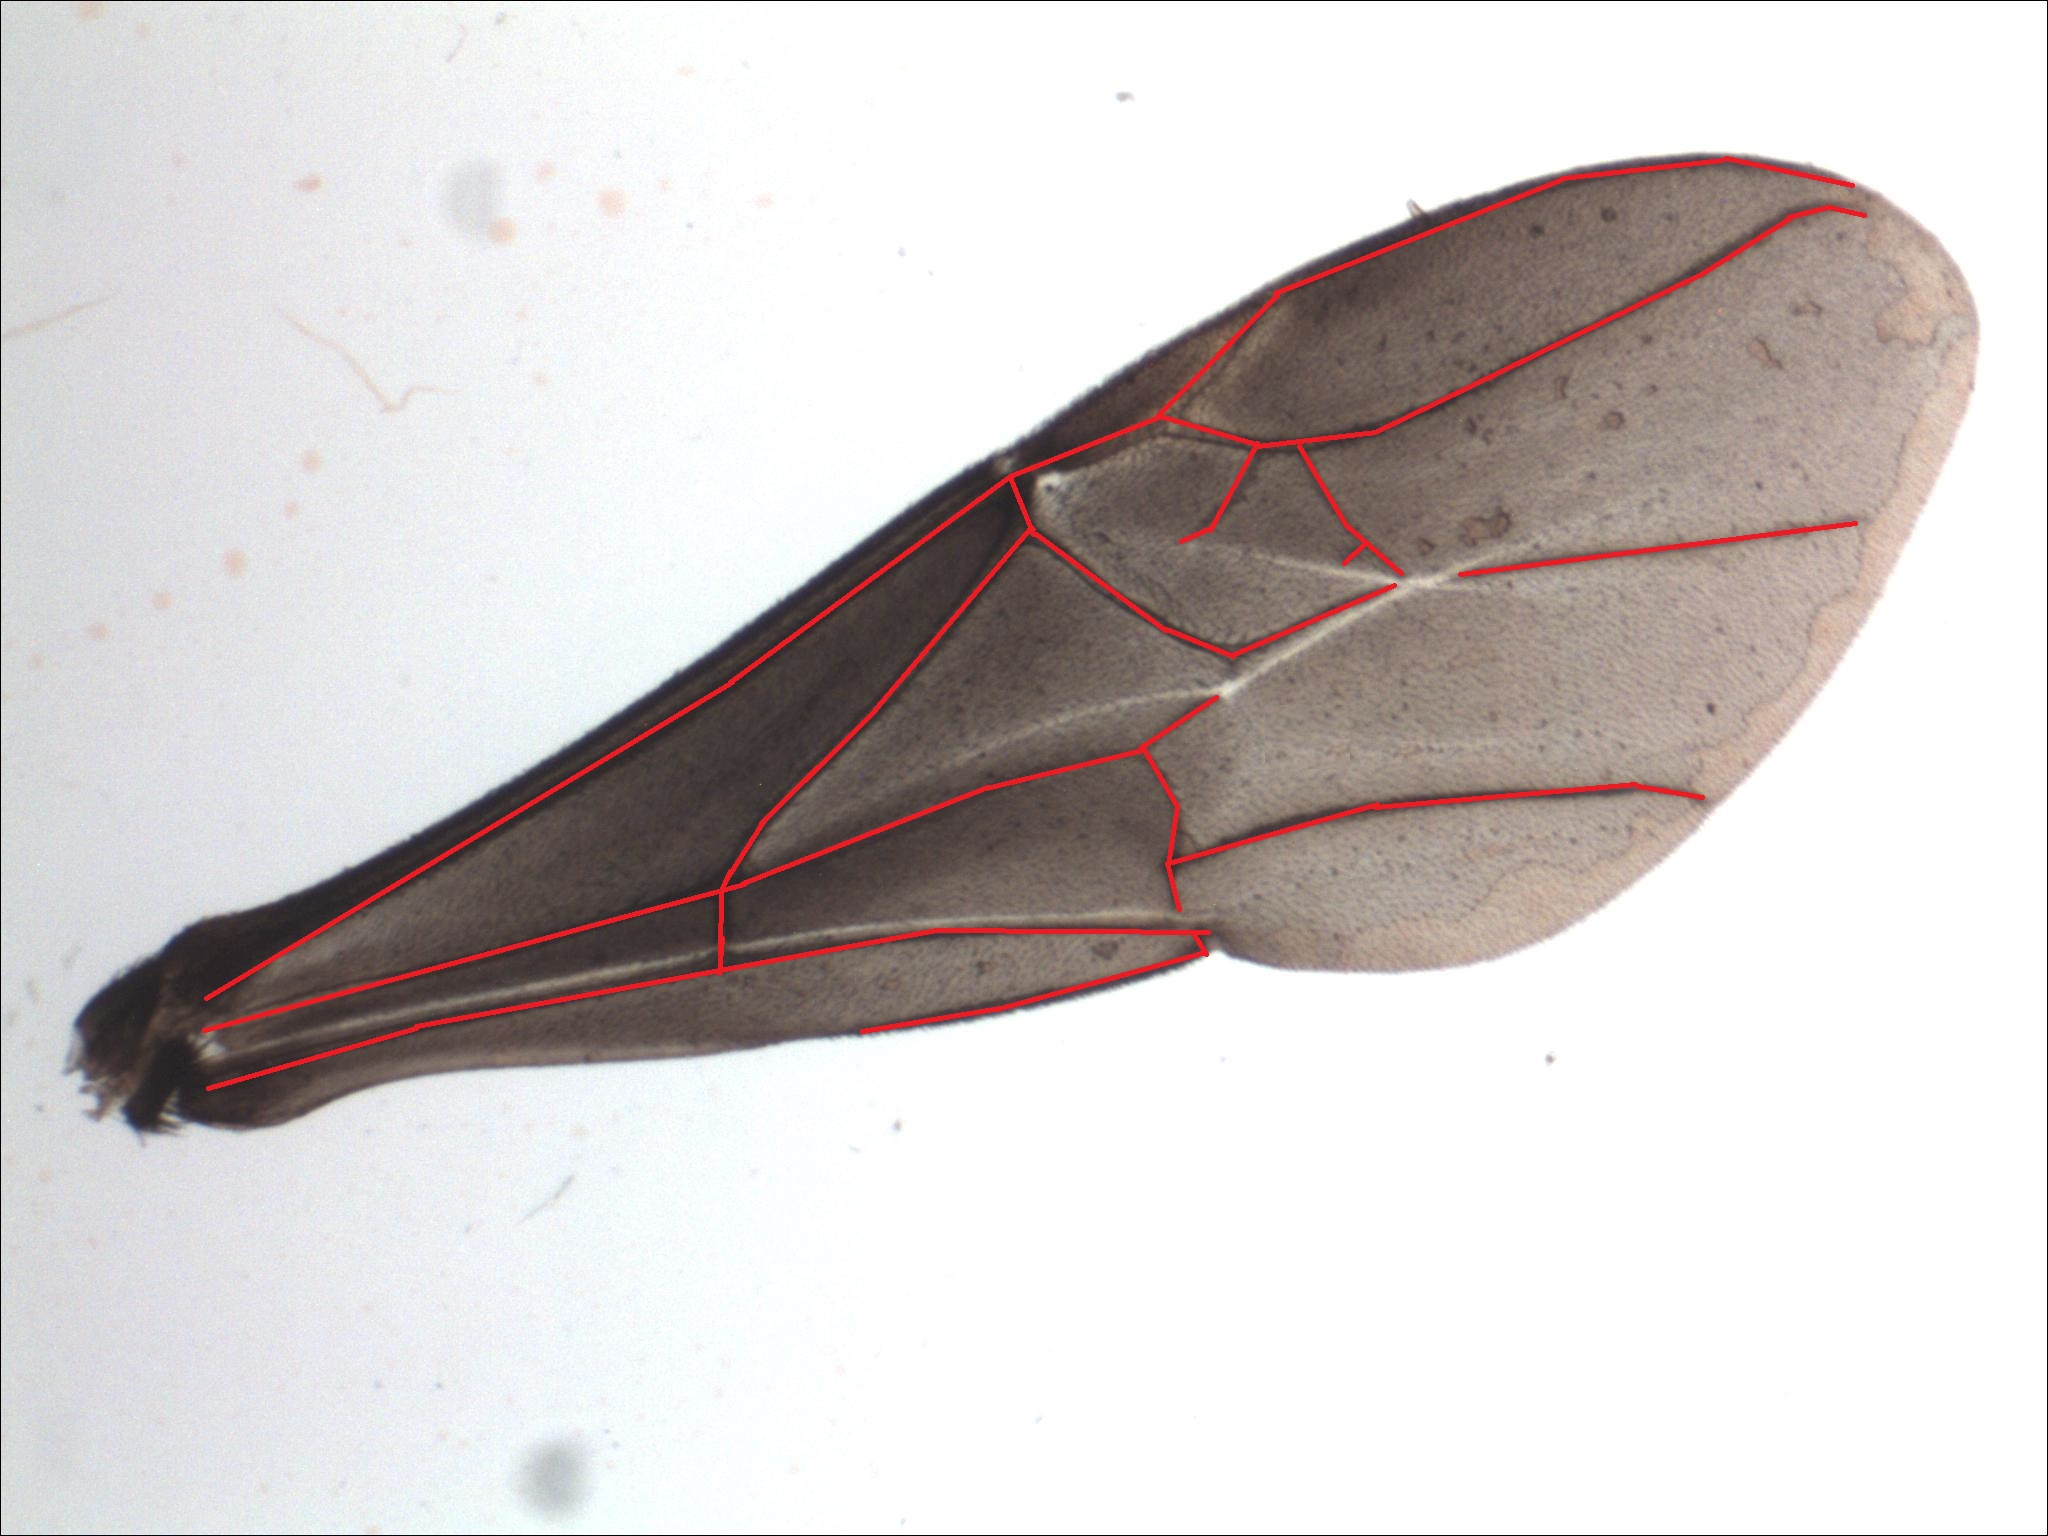
\includegraphics[width=.45\textwidth]{imagens/materiais_metodos/02_mel_trigona_spinipes_mapped.jpg}
    \label{fig:02_mel_trigona_spinipes}
    \source{Danilo Assunção, 2021}
\end{figure}

O conjunto de dados disponibilizado é constituído por um total de 904 imagens, sendo estas imagens uma representação digital das asas de várias espécies de abelhas e de um gênero específico de vespa. A partir deste conjunto de dados é apresentado um total de 22 gêneros que agrupam as espécies de abelhas, somando um total de 45 espécies e 3 espécies de vespas do mesmo gênero. Cada espécie corresponde nesse conjunto de dados tem uma classe que será tratada no modelo em questão. Estas especificações podem ser vistas na Tabela \ref{tab:conjunto_dados_abelhas}.

\begin{longtable}[c]{|l|l|r|}
\caption{Conjunto de dados original das asas de abelhas}
\label{tab:conjunto_dados_abelhas}\\
\hline
\multicolumn{1}{|c|}{Tribo}  & \multicolumn{1}{c|}{Gênero + Espécie}                & \multicolumn{1}{c|}{Quantidade de imagens} \\ \hline
\endfirsthead
%
\endhead
%
\multirow{6}{*}{Euglossini} 
                       & Eufriesea violacea  & 20 \\ \cline{2-3} 
                       & Euglossa mixta      & 20 \\ \cline{2-3} 
                       & Euglossa annectans  & 19 \\ \cline{2-3} 
                       & Euglossa truncata   & 15 \\ \cline{2-3} 
                       & Eulaema nigrita     & 10 \\ \cline{2-3} 
                       & Exaerete smaragdina & 8  \\ \hline
\multirow{4}{*}{Apini} & Apis cerana         & 20 \\ \cline{2-3} 
                       & Apis dorsata        & 20 \\ \cline{2-3} 
                       & Apis florea         & 20 \\ \cline{2-3} 
                       & Apis mellifera      & 19 \\ \hline
\multirow{2}{*}{Bombini}     
                       & Bombus (Fervidobombus) brasiliensis & 20 \\ \cline{2-3} 
                       & Bombus (Fervidobombus) pauloensis   & 11 \\ \hline
\multirow{33}{*}{Meliponini} 
                       & Austroplebeia australis            & 18 \\ \cline{2-3} 
                       & Austroplebeia cincta               & 20 \\ \cline{2-3} 
                       & Austroplebeia essinatoni           & 20 \\ \cline{2-3} 
                       & Austroplebeia striped              & 20 \\ \cline{2-3} 
                       & Austroplebeia symei                & 20 \\ \cline{2-3} 
                       & Axestotrigona ferrugínea           & 20 \\ \cline{2-3} 
                       & Dactylurina staudingeri            & 20 \\ \cline{2-3} 
                       & Geotrigona sp                      & 16 \\ \cline{2-3} 
                       & Lestrimelitta limao                & 19 \\ \cline{2-3} 
                       & Melipona (Eomelipona) bicolor      & 14 \\ \cline{2-3} 
                       & Melipona mandacaia                 & 20 \\ \cline{2-3} 
                       & Melipona quadrifasciata            & 20 \\ \cline{2-3} 
                       & Melipona subnitida                 & 19 \\ \cline{2-3} 
                       & Melipona (Michmelia) flavolineata  & 20 \\ \cline{2-3} 
                       & Melipona (Michmelia) scutellaris   & 20 \\ \cline{2-3} 
                       & Melipona seminigra seminigra       & 20 \\ \cline{2-3} 
                       & Meliponula bocandei                & 20 \\ \cline{2-3} 
                       & Mourella caerulea                  & 20 \\ \cline{2-3} 
                       & Nannotrigona testaceicornis        & 20 \\ \cline{2-3} 
                       & Paratrigona subnuda                & 20 \\ \cline{2-3} 
                       & Partamona helleri                  & 20 \\ \cline{2-3} 
                       & Plebeia droryana                   & 20 \\ \cline{2-3} 
                       & Plebeia flavocincta                & 19 \\ \cline{2-3} 
                       & Plebeia nigriceps                  & 20 \\ \cline{2-3} 
                       & Plebeia pugnax                     & 20 \\ \cline{2-3} 
                       & Plebeia remota                     & 20 \\ \cline{2-3} 
                       & Plebeia sp                         & 20 \\ \cline{2-3} 
                       & Scaptotrigona bipunctata           & 20 \\ \cline{2-3} 
                       & Scaptotrigona depilis              & 20 \\ \cline{2-3} 
                       & Scaptotrigona tubiba               & 19 \\ \cline{2-3} 
                       & Scaura latitarsis                  & 20 \\ \cline{2-3} 
                       & Schwarziana quadripunctata         & 19 \\ \cline{2-3} 
                       & Trigona spinipes                   & 20 \\ \hline
\multirow{3}{*}{Trypoxylini} 
                       & Trypoxylon aurifrons   & 20 \\ \cline{2-3} 
                       & Trypoxylon lactitarse  & 20 \\ \cline{2-3} 
                       & Trypoxylon rogenhoferi & 20 \\ \hline

\multicolumn{3}{|c|}{Fonte - Danilo Assunção, 2022} \\ \hline
\end{longtable}

Conforme apresentado, para levantar o estado da arte para o uso de uma arquitetura de CNN em união com uma técnica de transferência de aprendizado e técnicas de aumento de dados para realizar a identificação automática de espécie de abelhas, foi elaborada uma revisão sistemática utilizando os conceitos aplicados em \citeonline{liu2020classification}.

Após o levantamento do estado da arte, foi construída uma ferramenta (\href{https://github.com/danilo-assuncao/bee-masters-project/tree/main/tools/colab-notebooks}{\textit{pipeline}}) constituída de dois módulos essenciais, o primeiro módulo sendo o responsável pela geração dos conjuntos de dados de treinamento, validação e teste em cima do conjunto de dados original formado pelas 904 imagens, em que o conjunto de treinamento terá seu volume aumentado através do uso de técnicas de aumento de dados, e o segundo módulo que aplicará a configuração, seleção da arquitetura de CNN e execução do modelo para ser trabalhado em cima dos conjuntos de dados organizados pelo primeiro módulo.

\section{Módulo do conjunto de dados}
Este primeiro módulo consiste em extrair, organizar, dividir, compactar e armazenar o conjunto de dados criado. Os passos executados por este módulo podem ser vistos na Figura \ref{fig:diagrama_modulo_do_conjunto_dados}.

\begin{figure}[H]
    \centering
    \caption{Representação do módulo do conjunto de dados}
    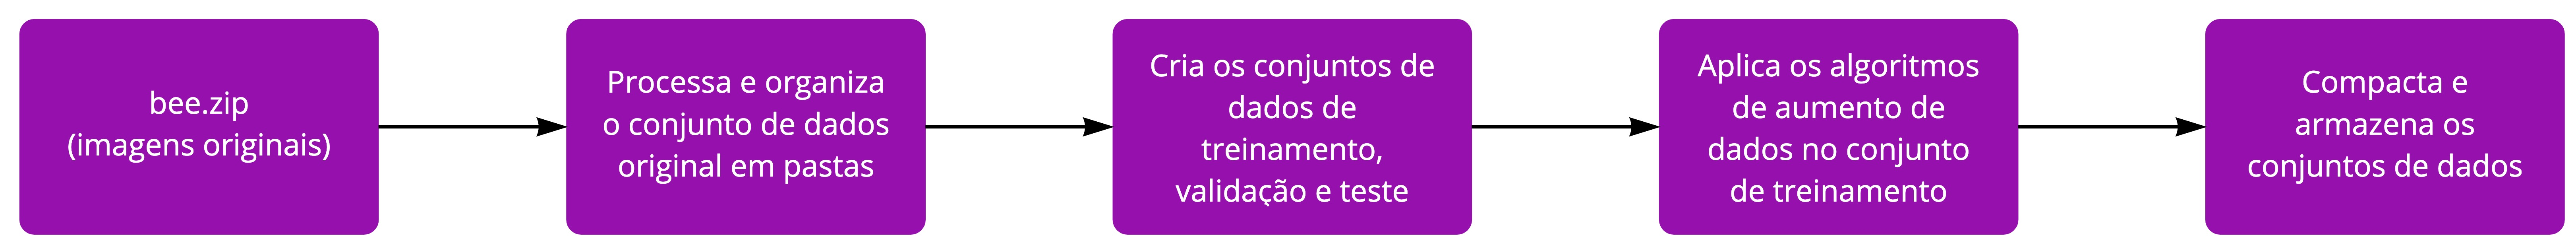
\includegraphics[width=1.0\textwidth]{imagens/materiais_metodos/modulo_conjunto_dados/pipeline_geracao_do_dataset.jpg}
    \label{fig:diagrama_modulo_do_conjunto_dados}
    \source{Danilo Assunção, 2022}
\end{figure}

Conforme exibido na Figura \ref{fig:diagrama_modulo_do_conjunto_dados}, este módulo foi dividido em cinco etapas de execução, onde cada quadrado roxo representa uma etapa. Estas etapas são definidas como:

\begin{enumerate}
  \item Carregamento dos dados originais;
  \item Processamento e organização do conjunto de dados;
  \item Divisão dos conjuntos de dados;
  \item Aumento do conjunto de dados de treinamento;
  \item Compactação e armazenamento dos conjuntos de dados criados.
\end{enumerate}

No carregamento dos dados originais, é feito o carregamento do conjunto de dados originais contendo as 904 imagens que será transformada em uma representação computacional a qual a ferramenta que irá processar o conteúdo possa computar tais imagens.

Na etapa de processamento e organização do conjunto de dados, as imagens previamente carregadas foram organizadas automaticamente em uma estrutura de diretórios, em que cada diretório representa uma determinada espécie de abelha contendo suas respectivas imagens, conforme apresentado na Figura \ref{fig:pipeline_geracao_do_dataset_processamento_dados}.

\begin{figure}[H]
    \centering
    \caption{Processamento e organização das imagens}
    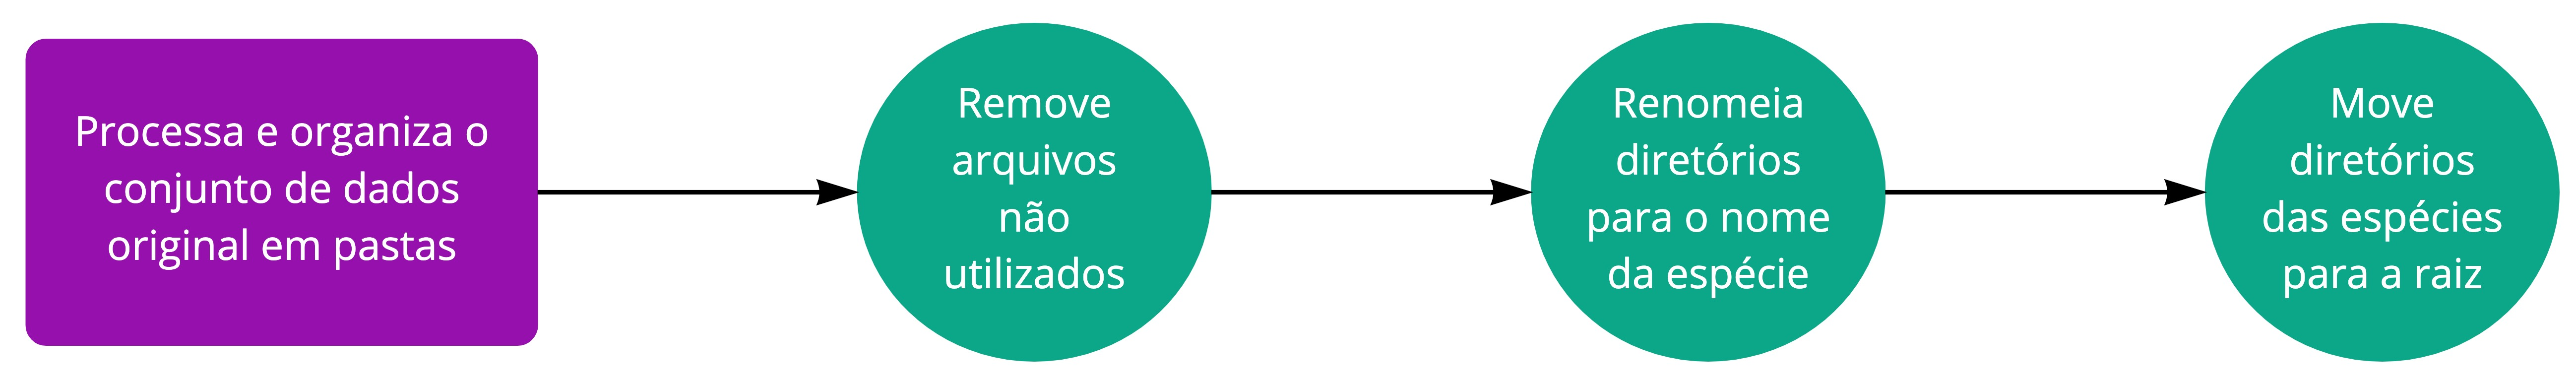
\includegraphics[width=1.0\textwidth]{imagens/materiais_metodos/modulo_conjunto_dados/pipeline_geracao_do_dataset_processamento_dados.jpg}
    \label{fig:pipeline_geracao_do_dataset_processamento_dados}
    \source{Danilo Assunção, 2022}
\end{figure}

Na etapa de divisão dos conjuntos de dados, é feito um agrupamento de um número determinado pelo percentual com base no total de imagens disponíveis para diretórios que representam o conjunto de treinamento, validação e teste. Tal divisão é feita selecionando 60\% das imagens disponíveis para o conjunto de dados de treinamento, 20\% das imagens para o conjunto de dados de validação e por fim os últimos 20\% das imagens restantes são direcionadas para o conjunto de dados de teste, esta representação pode ser vista na Figura \ref{fig:pipeline_geracao_do_dataset_divisao}.

\begin{figure}[H]
    \centering
    \caption{Divisão dos conjuntos de dados}
    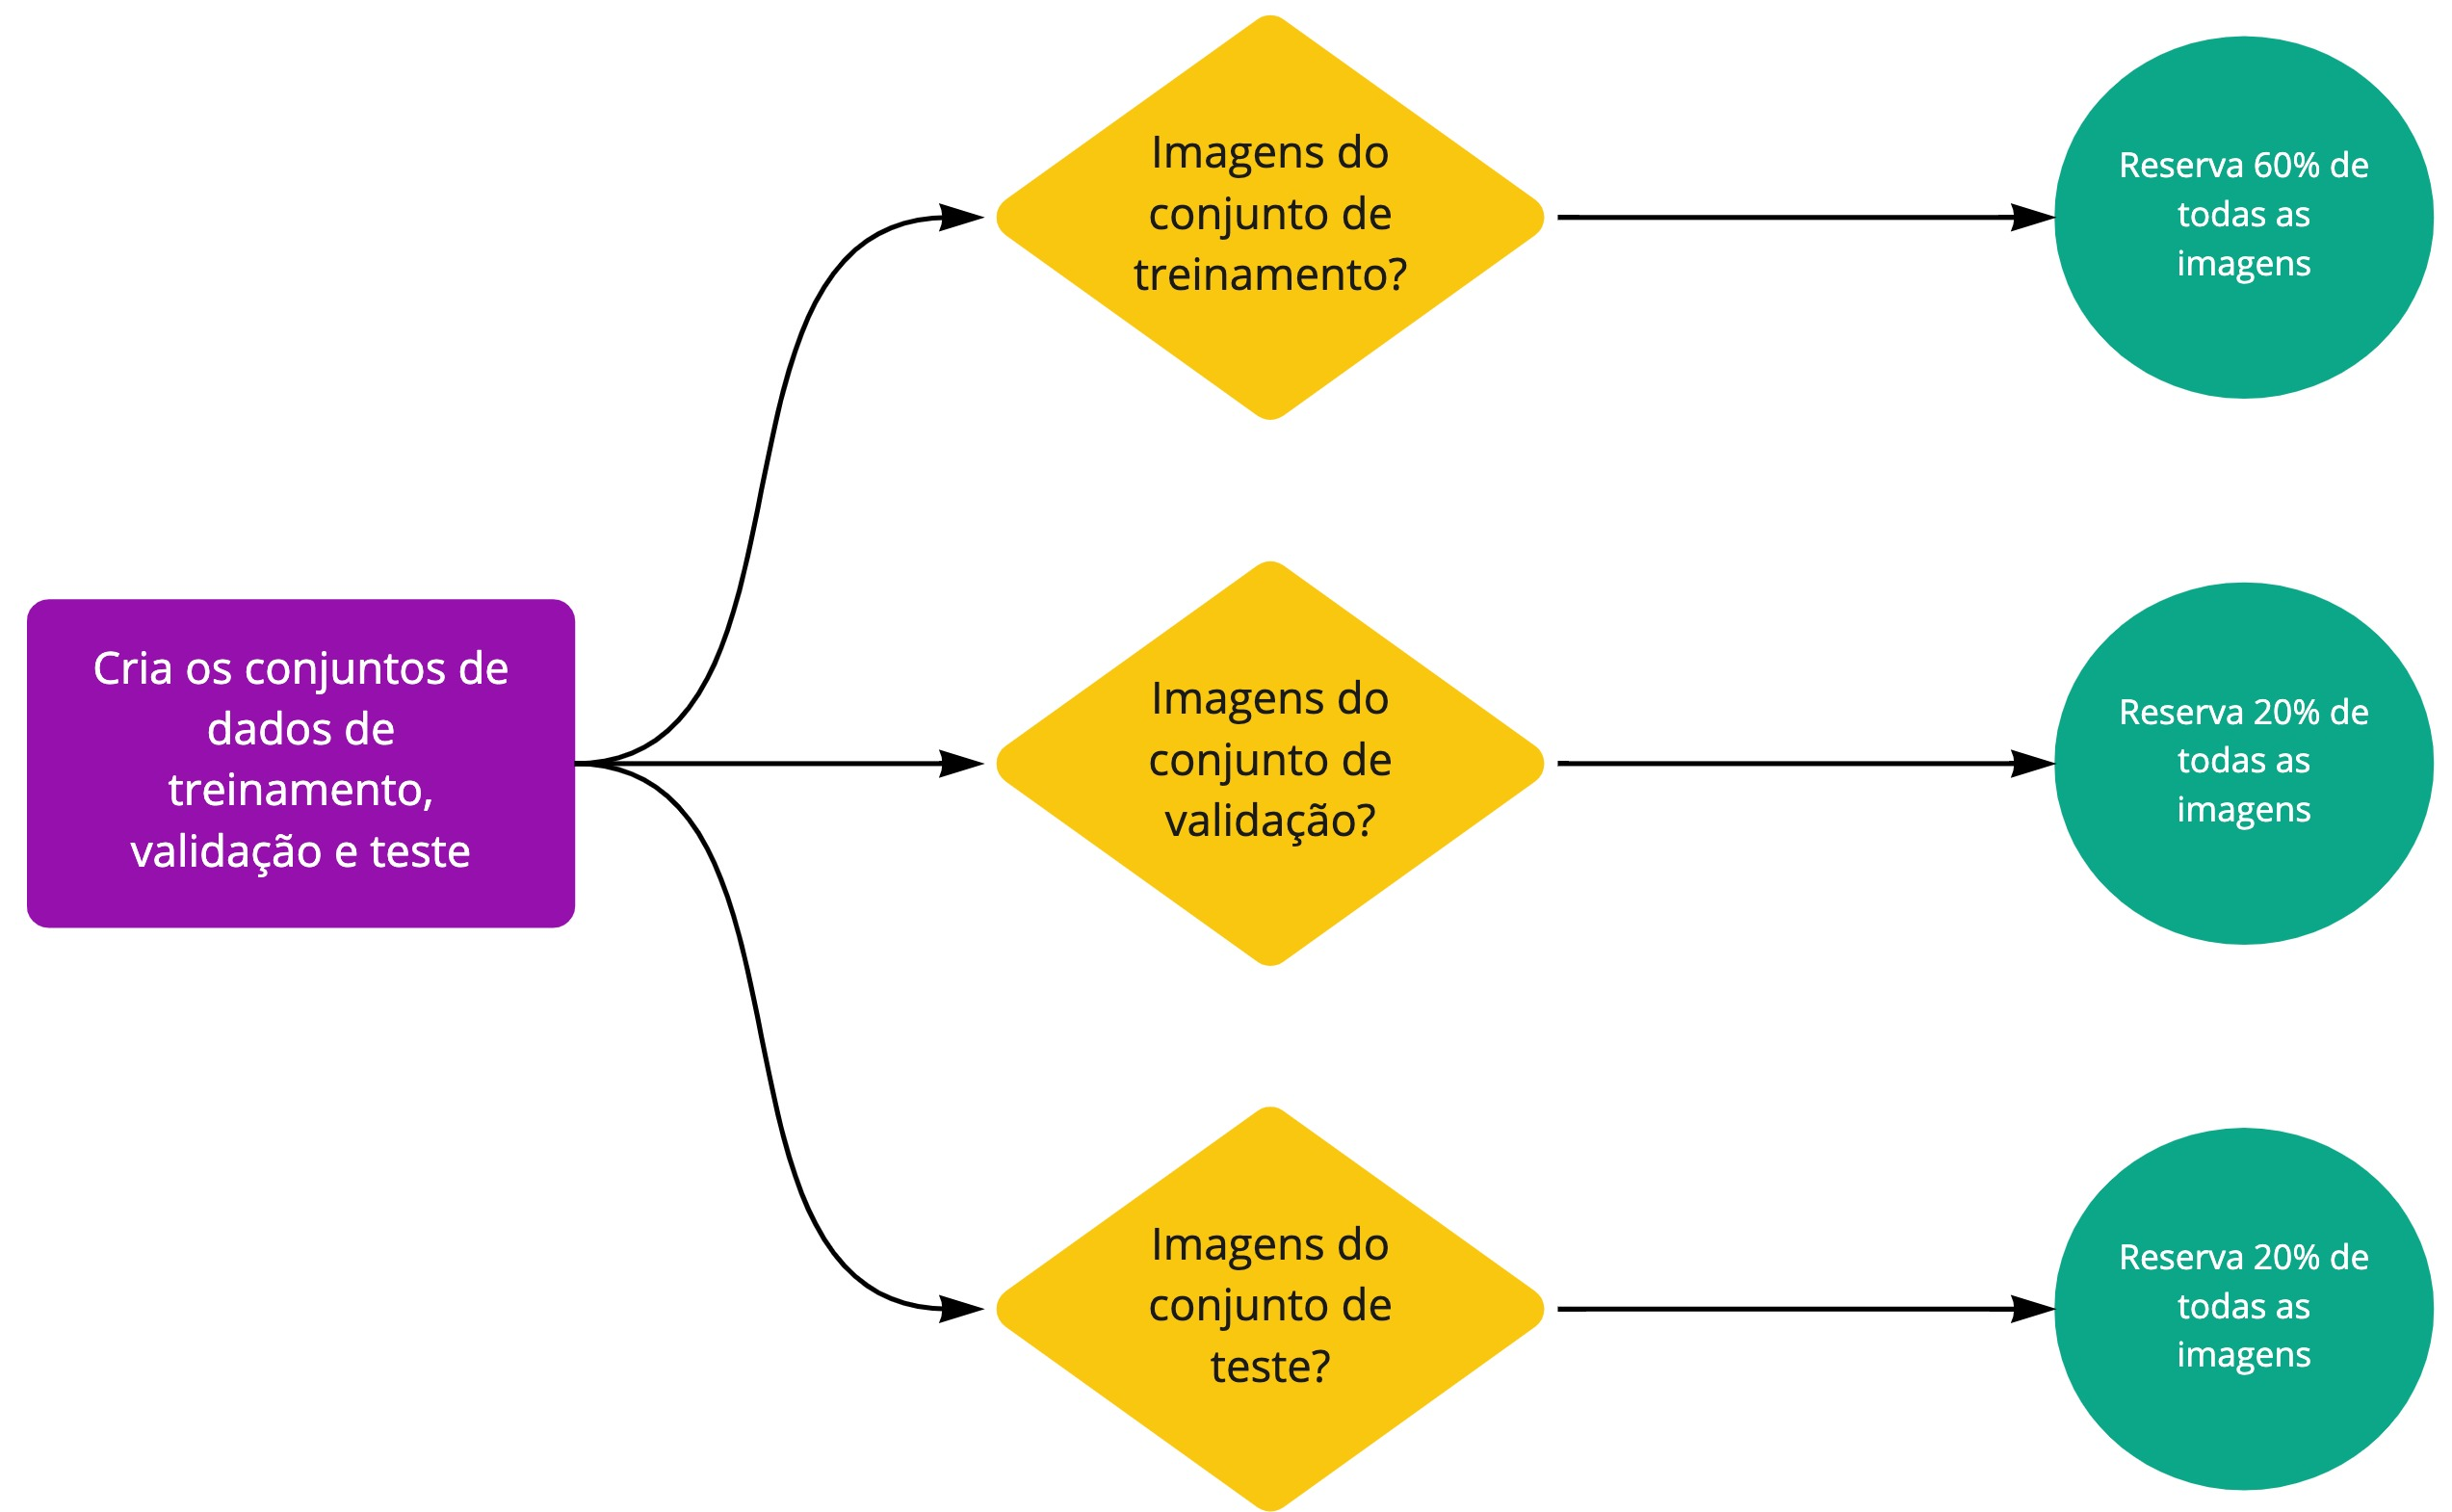
\includegraphics[width=1.0\textwidth]{imagens/materiais_metodos/modulo_conjunto_dados/pipeline_geracao_do_dataset_divisao.jpg}
    \label{fig:pipeline_geracao_do_dataset_divisao}
    \source{Danilo Assunção, 2022}
\end{figure}

Na etapa de aumento do conjunto de dados de treinamento, é feito a aplicação de algoritmos de aumento de dados no conjunto de dados de treinamento e este procedimento é feito aplicando algoritmos que cria uma nova imagem alterando a propriedade base da imagem original utilizando métodos como, alteração do nível de saturação, inversão horizontal, inversão vertical, alteração na escala de cinza, alteração do brilho, corte central e rotação de 90 graus e estes métodos permitem que todo o conjunto de dados de treinamento seja multiplicado em 7 vezes o seu tamanho original seja replicada em mais outras 7 imagens. Este método permitiu que o conjunto de dados de treinamento original aumentasse de 544, sendo este número de imagens o resultado do arredondamento que representa os 60\% do conjunto de dados original, para 3.808 imagens e tais métodos aplicados para este aumento representados pelos círculos azuis na Figura \ref{fig:pipeline_geracao_do_dataset_aumento_de_dados} são categorizados como métodos de transformação geométrica e foram selecionados para uso neste trabalho devido a sua facilidade de implementação \cite{shorten2019survey}. O procedimento completo desta etapa pode ser visto na Figura \ref{fig:pipeline_geracao_do_dataset_aumento_de_dados}.

\begin{figure}[H]
    \centering
    \caption{Aumento do conjunto de dados de treinamento}
    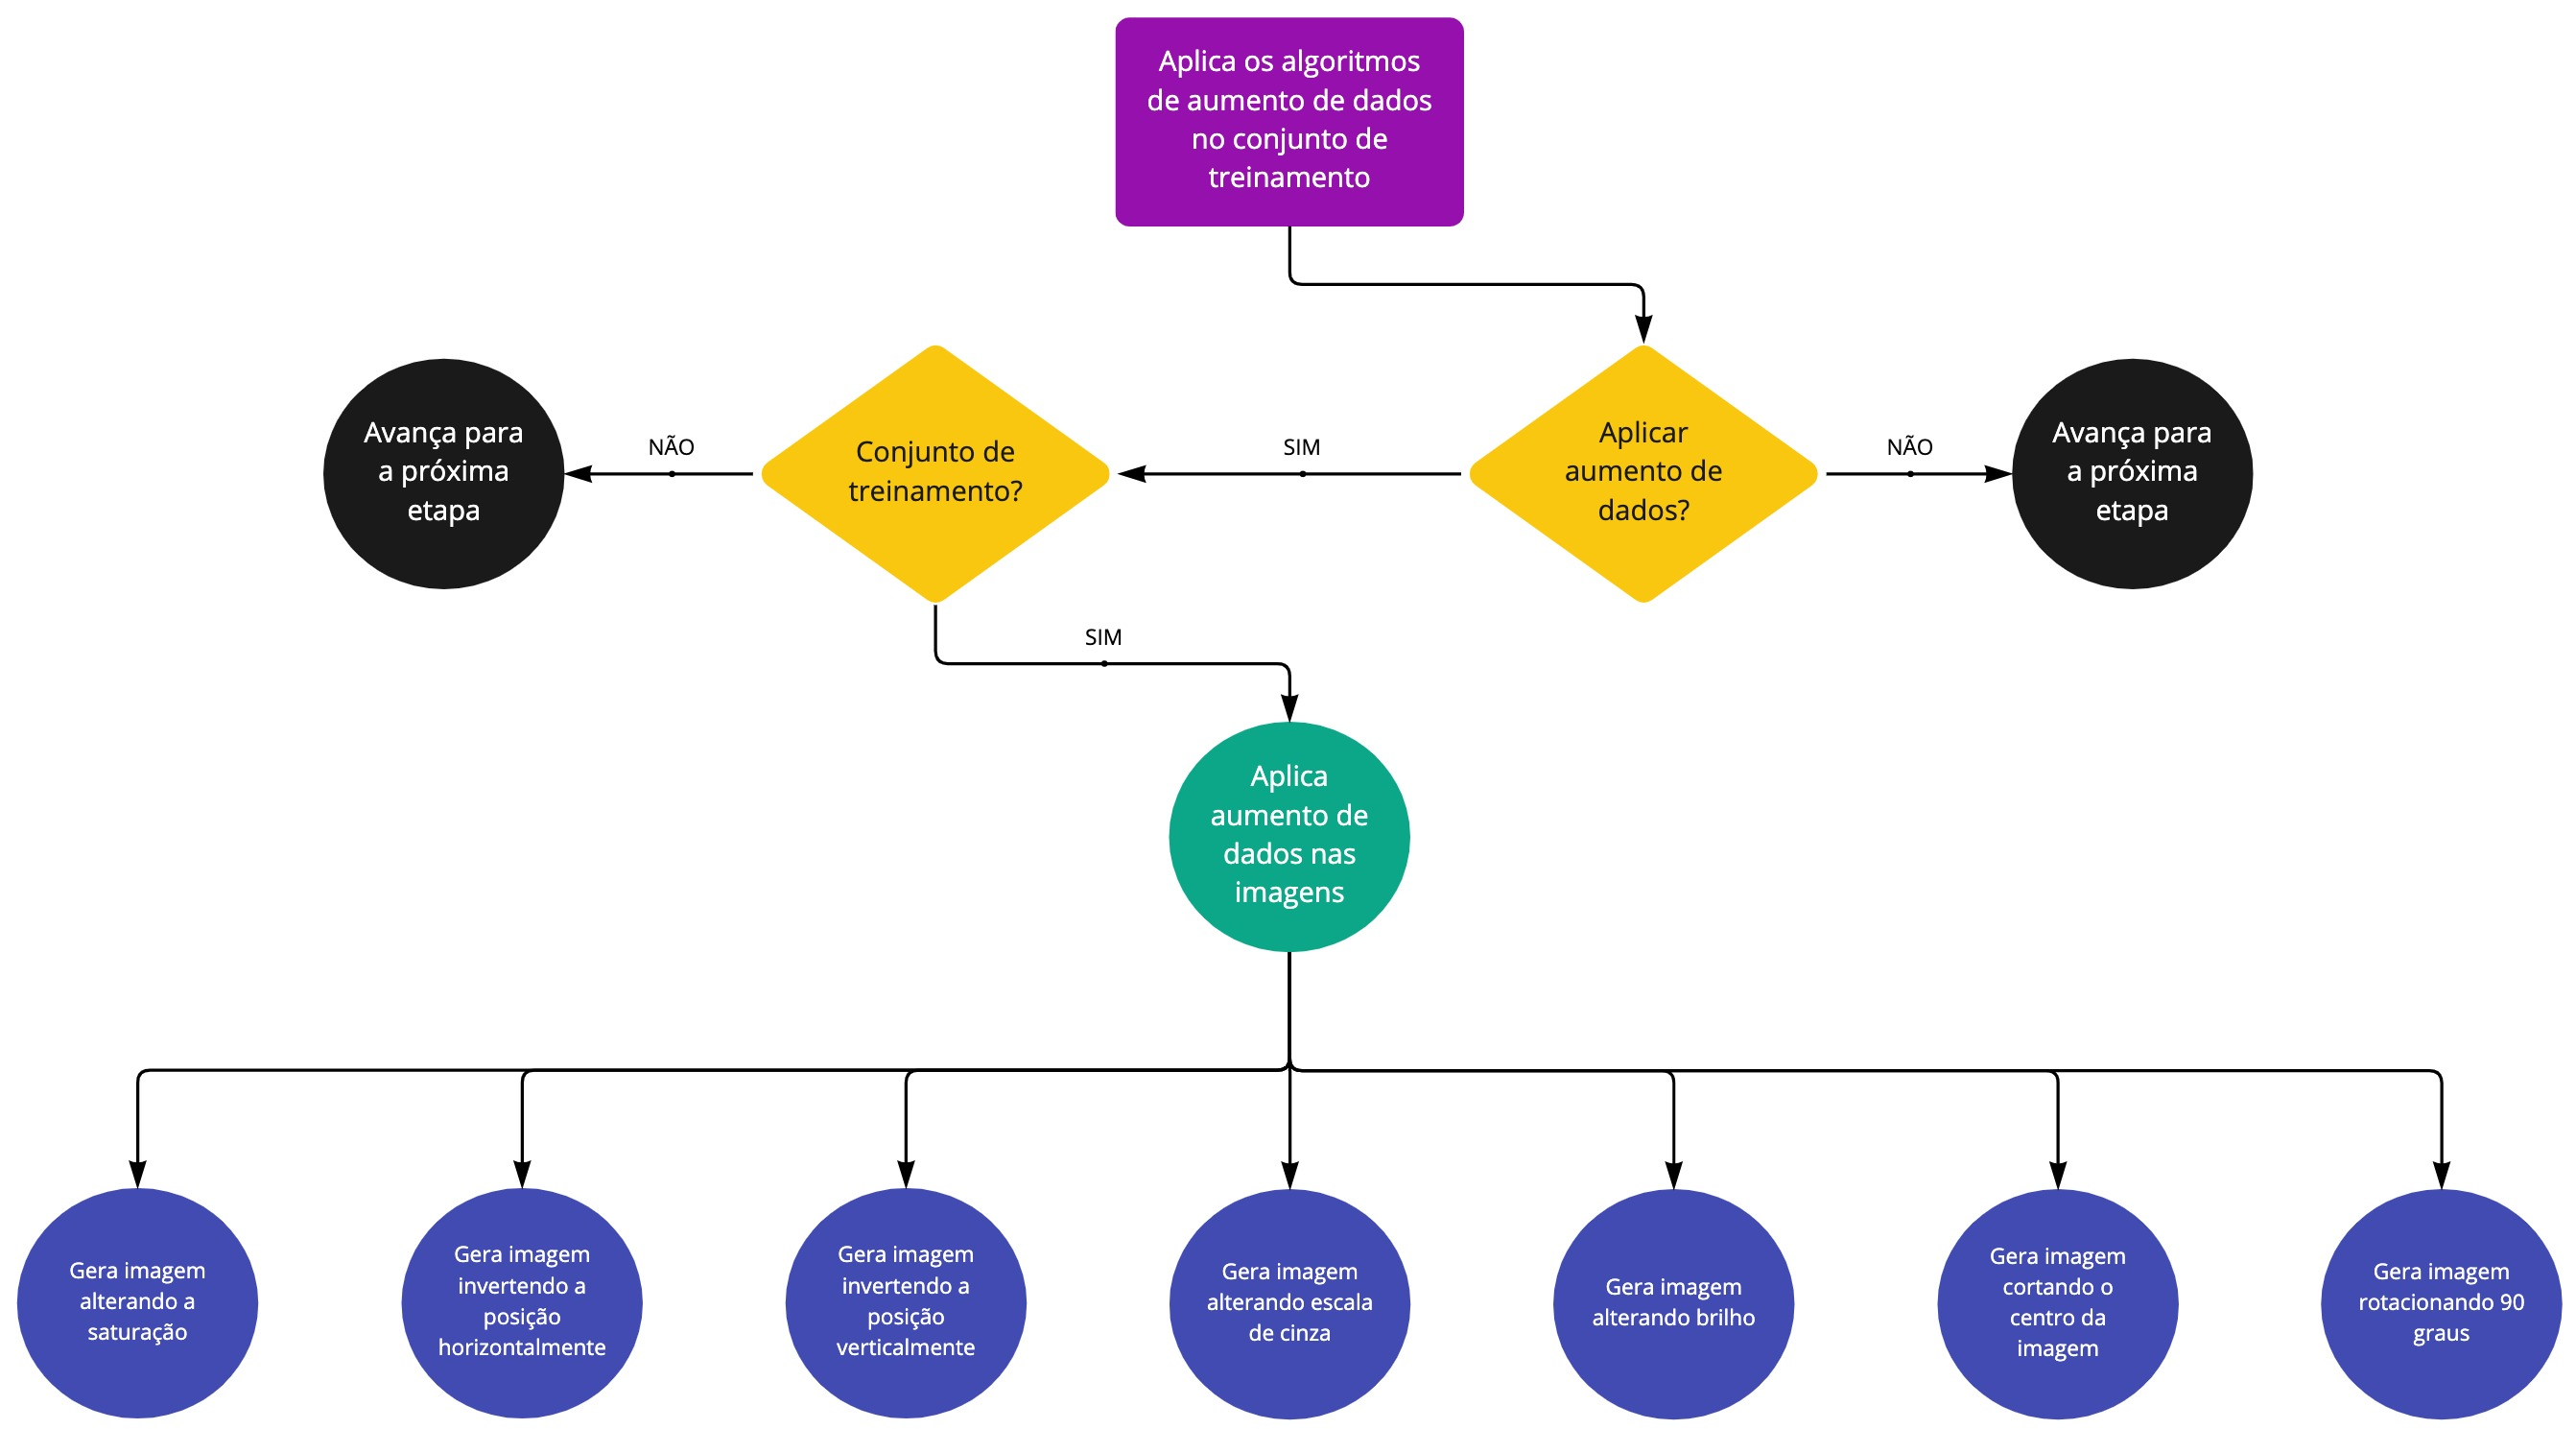
\includegraphics[width=1.0\textwidth]{imagens/materiais_metodos/modulo_conjunto_dados/pipeline_geracao_do_dataset_aumento_de_dados.jpg}
    \label{fig:pipeline_geracao_do_dataset_aumento_de_dados}
    \source{Danilo Assunção, 2022}
\end{figure}

Na etapa de compactação e armazenamento do conjunto de dados, é realizado o agrupamento de todos os conjuntos de dados criados em um diretório onde tal diretório é compactado e armazenado na nuvem (\textit{Google Drive}). Esses passos podem ser vistos na Figura \ref{fig:pipeline_geracao_do_dataset_compacta}.

\begin{figure}[H]
    \centering
    \caption{Compactação e armazenamento do conjunto de dados}
    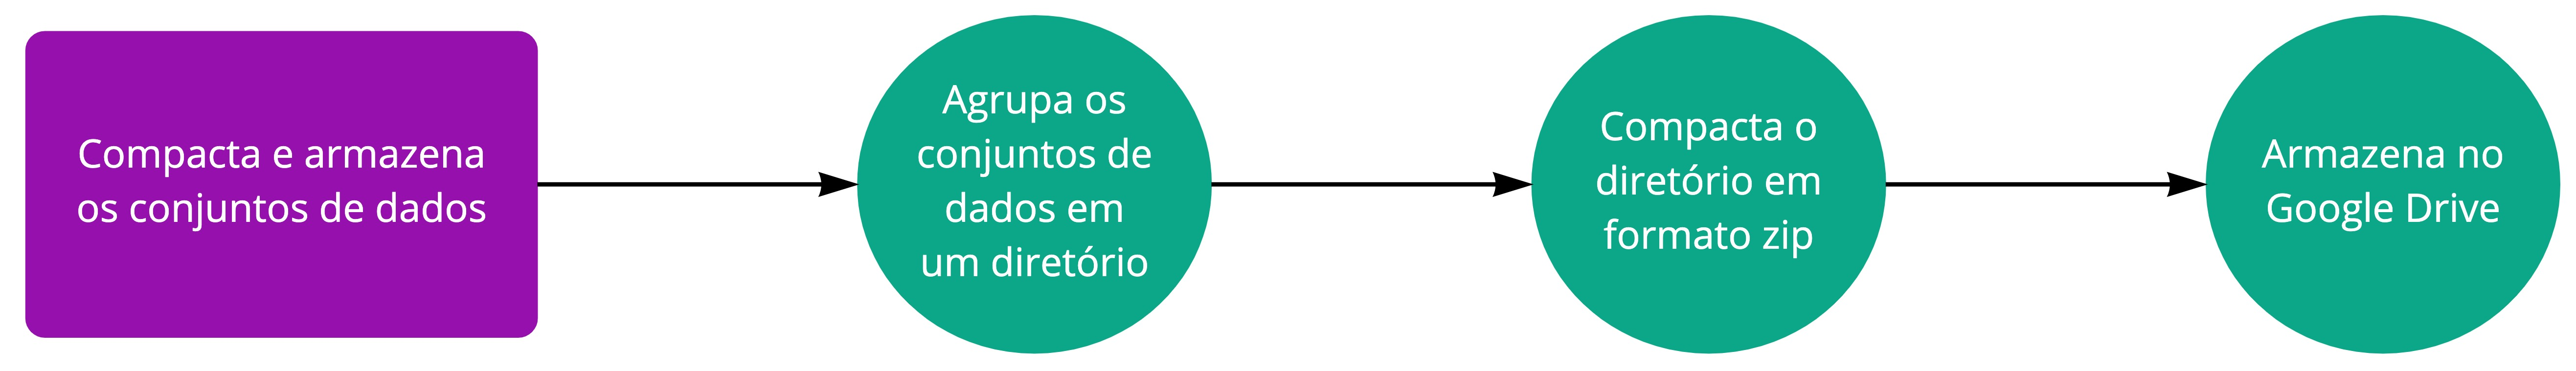
\includegraphics[width=1.0\textwidth]{imagens/materiais_metodos/modulo_conjunto_dados/pipeline_geracao_do_dataset_compacta.jpg}
    \label{fig:pipeline_geracao_do_dataset_compacta}
    \source{Danilo Assunção, 2022}
\end{figure}

\section{Módulo do modelo de classificação}
O módulo do modelo de classificação possui a responsabilidade de consumir o conjunto de dados pré-processado pelo módulo do conjunto de dados, configurar, selecionar uma arquitetura de CNN e executá-la com o conjunto de dados carregado, testar e exibir os resultados de todos os passos executados. Como é possível observar através da Figura \ref{fig:pipeline_model_cnn}, este módulo é dividido em quatro grupos de execução, sendo estes grupos, Configuração; Definição do modelo; Treinamento e validação e por fim o Teste.

\begin{figure}[H]
    \centering
    \caption{Representação do módulo do modelo de classificação}
    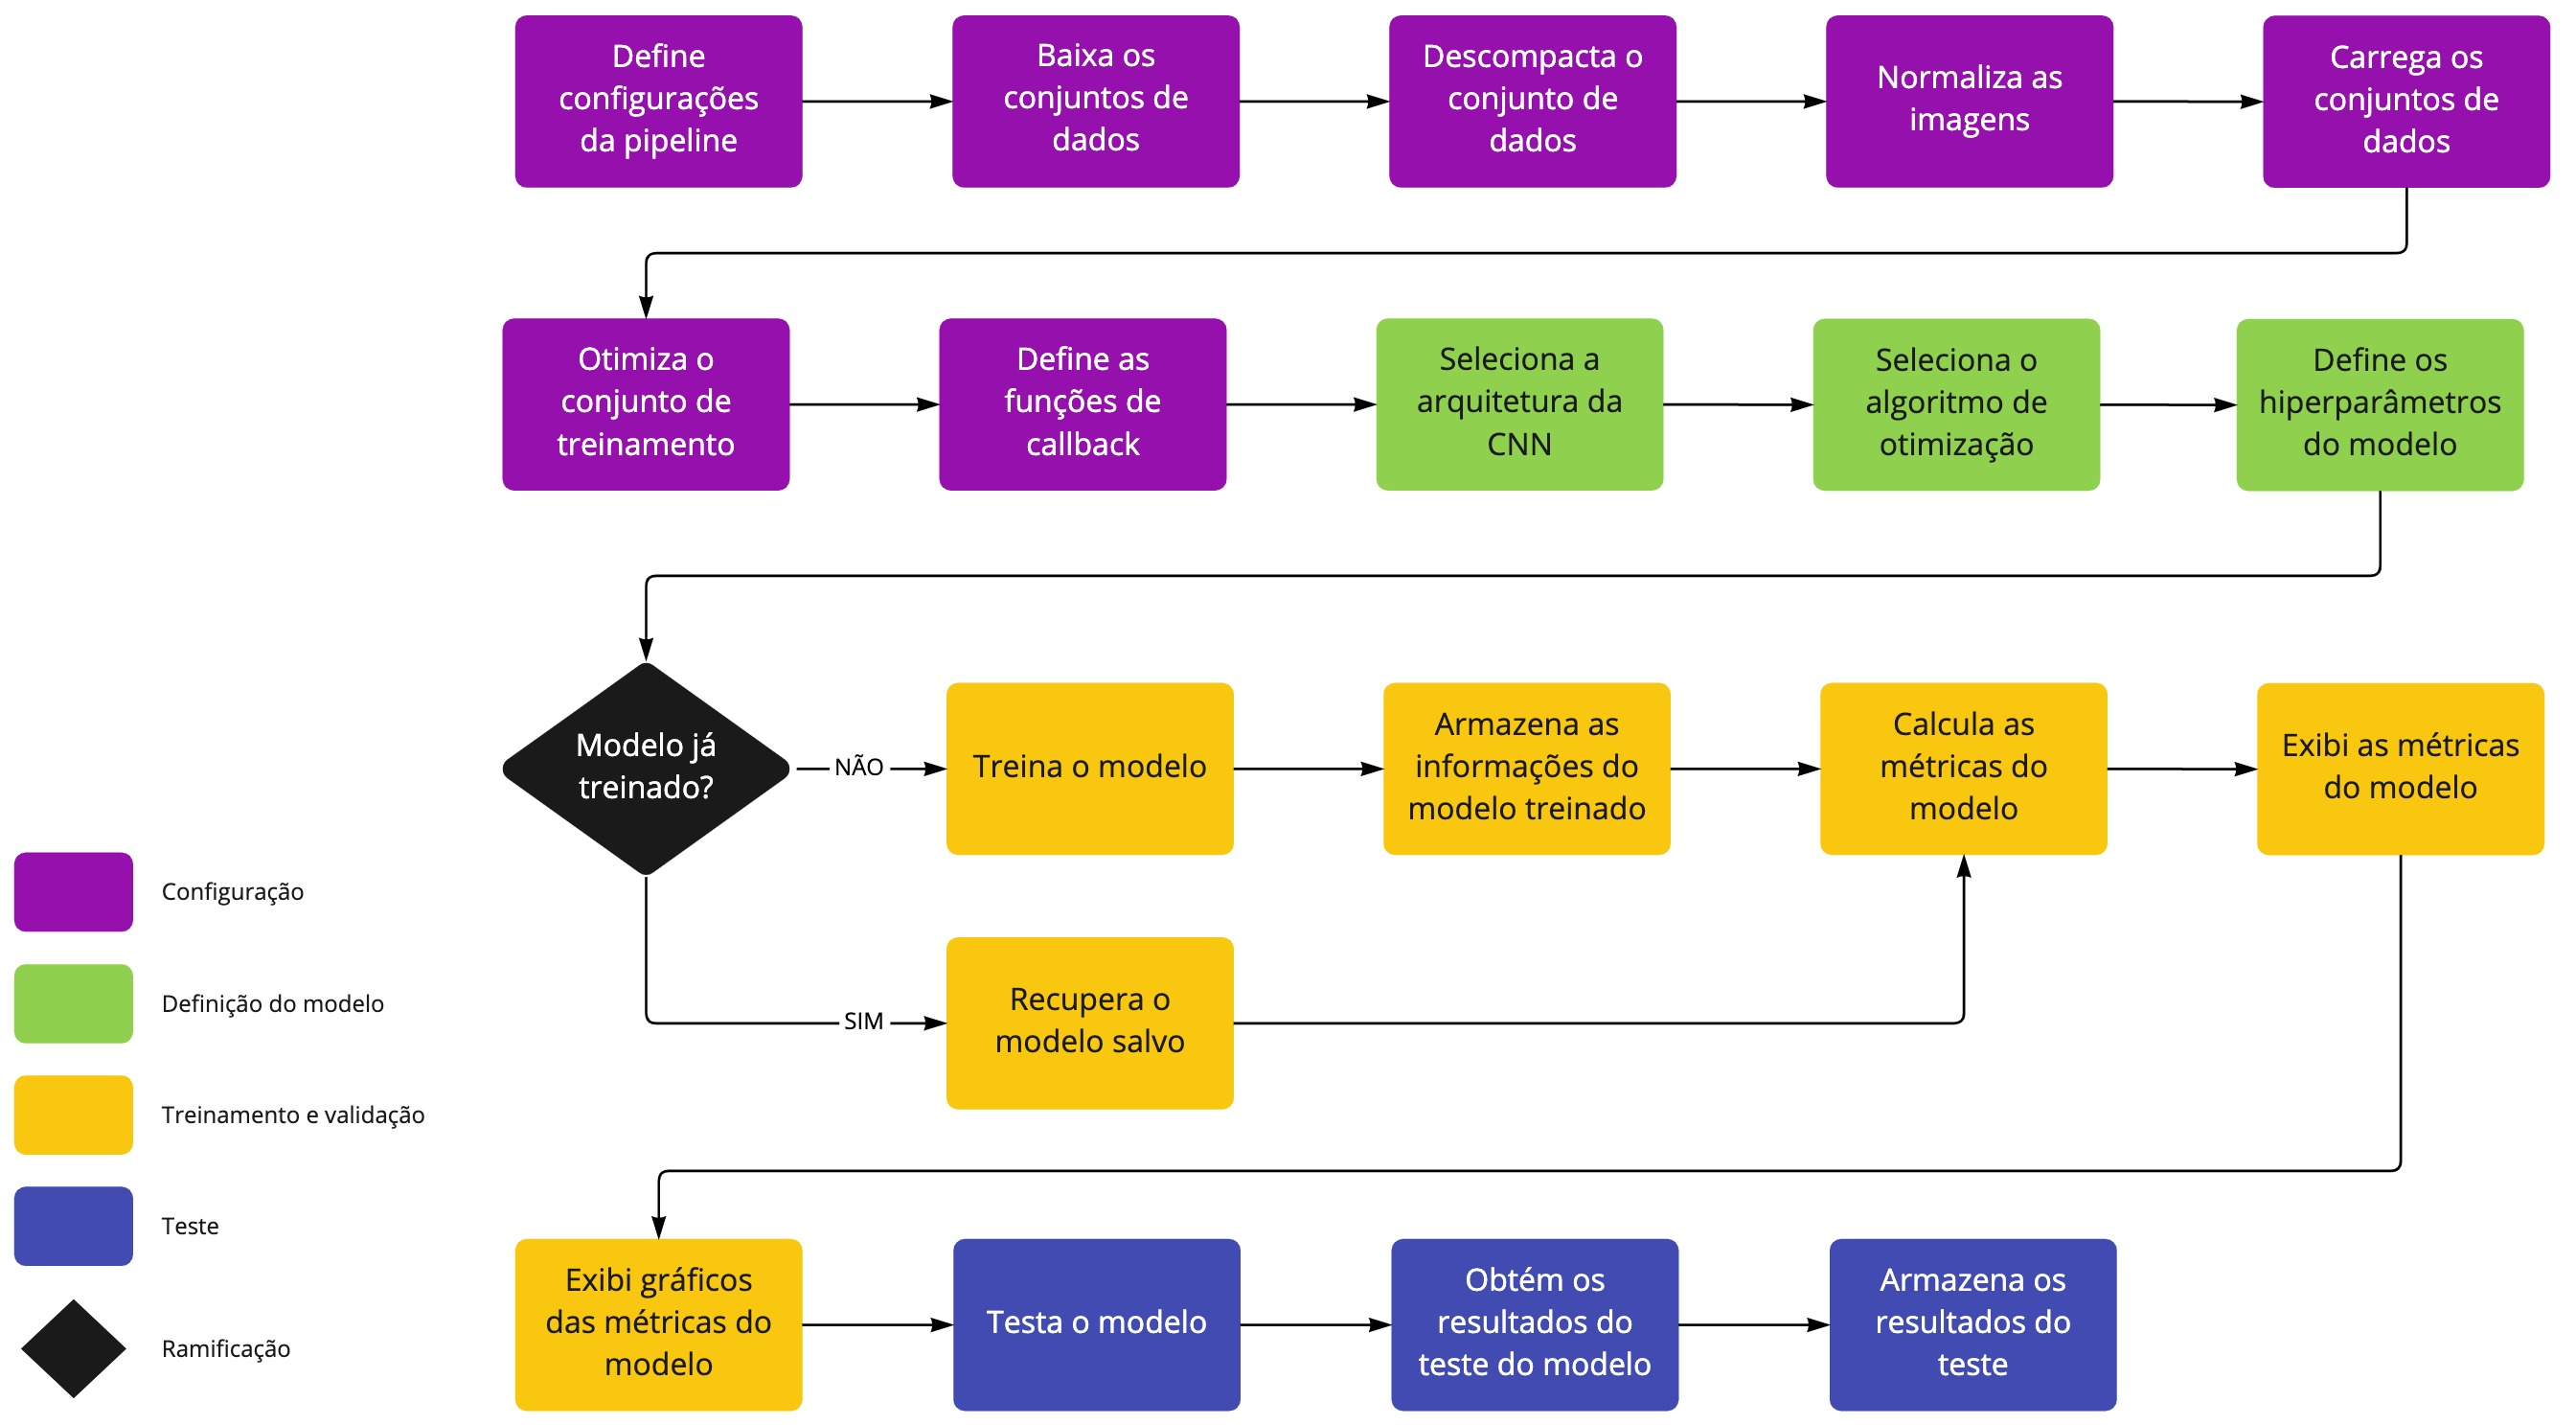
\includegraphics[width=1.0\textwidth]{imagens/materiais_metodos/modulo_modelo/pipeline_modelo_cnn.jpg}
    \label{fig:pipeline_model_cnn}
    \source{Danilo Assunção, 2022}
\end{figure}

\subsection{Grupo de configuração}
O grupo de configuração tem como objetivo determinar todos os parâmetros necessários deste módulo e, também, extrair e carregar o conjunto de dados pré-processado, otimizar e configurar funções de \textit{callback} (funções personalizadas chamadas durante o processo de execução), como pode ser visto na Figura \ref{fig:pipeline_modelo_cnn_grupo_configuração}.

\begin{figure}[H]
    \centering
    \caption{Grupo de configuração}
    \includegraphics[width=1.0\textwidth]{imagens/materiais_metodos/modulo_modelo/pipeline_modelo_cnn_grupo_configuração.jpg}
    \label{fig:pipeline_modelo_cnn_grupo_configuração}
    \source{Danilo Assunção, 2022}
\end{figure}

As configurações do \textit{pipeline} são constantes definidas contendo uma série de características presentes neste módulo, como a dimensão das imagens que serão trabalhadas, a localização de diretórios locais e na nuvem, e a parametrização para as condicionais executadas em pontos específicos, tendo como exemplo a exibição de \textit{logs} da ferramenta e alguns parâmetros gerais utilizados pelo modelo, tal como, o número de \textit{batches} por época. Então, é feito a transferência do conjunto de dados pré-processados através do \textit{Google Drive}, para assim o conjunto de dados ser descompactado e gerar três diretórios, contendo, cada um, o conjunto de dados de treinamento, validação e teste. Após a obtenção dos conjuntos de dados distintos, é realizado um processo de normalização nos \textit{pixels} das imagens de treinamento para valores compreendidos entre 0 e 1. Em seguida, os dados são carregados em estruturas que redimensionam e organizam as imagens em memória RAM, e, estas estruturas, são criadas e divididas em três partições, a de treinamento, validação e teste, em que, esses conjuntos de dados acabam por ter nestas estruturas a aplicação de um algoritmo que aleatoriamente embaralha as imagens contidas em cada um dos conjunto de dados. Após a criação destas estruturas, os dados presentes para treinamento são otimizados utilizando um mecanismo de \textit{cache}, para que o processo de leitura das imagens seja realizado de maneira mais otimizada a cada \textit{batch} de imagens que serão entregues ao ciclo de treinamento do modelo, e, por fim, algumas funções (\textit{callback functions}) são definidas para serem chamadas durante a execução do treinamento, sendo elas responsáveis por recuperar os resultados obtidos em cada época no processo de treinamento do modelo.

\subsection{Grupo de definição do modelo}
No grupo de definição do modelo, temos os passos responsáveis por selecionar a arquitetura de CNN que é utilizada na execução do modelo, sendo esta metodologia empregada visando a determinar dinamicamente as arquiteturas que serão utilizadas nos testes do modelo determinado. As arquiteturas de CNN foram escolhidas com base na revisão sistemática realizada neste trabalho, sendo elas, InceptionResnet v2, VGGNet 16, VGGNet 19, Resnet-152, Inception v3. Cada uma destas arquiteturas pode ou não utilizar uma técnica de transferência de aprendizado de ajuste fino, e para o uso desta técnica, será necessário o uso de pesos já pré-treinados. O método de ajuste fino foi escolhido como o método de transferência de aprendizado deste trabalho dado os aspectos positivos em seu uso especificados em \citeonline{li2017learning}. Em seguida, é feita a seleção dos algoritmos de otimização da CNN, tais algoritmos foram, Gradiente Descendente Estocástico (SGD), Adadelta, Adagrad, Adamax. Posteriormente é feita a definição dos hiperparâmetros do otimizador selecionado, para assim os parâmetros serem igualmente definidos para todas as arquiteturas propostas, tendo como exemplo a taxa de aprendizado. A representação desta etapa pode ser visualizada através da Figura \ref{fig:pipeline_modelo_cnn_grupo_definicao_modelo}.
 
\begin{figure}[H]
    \centering
    \caption{Grupo de definição do modelo}
    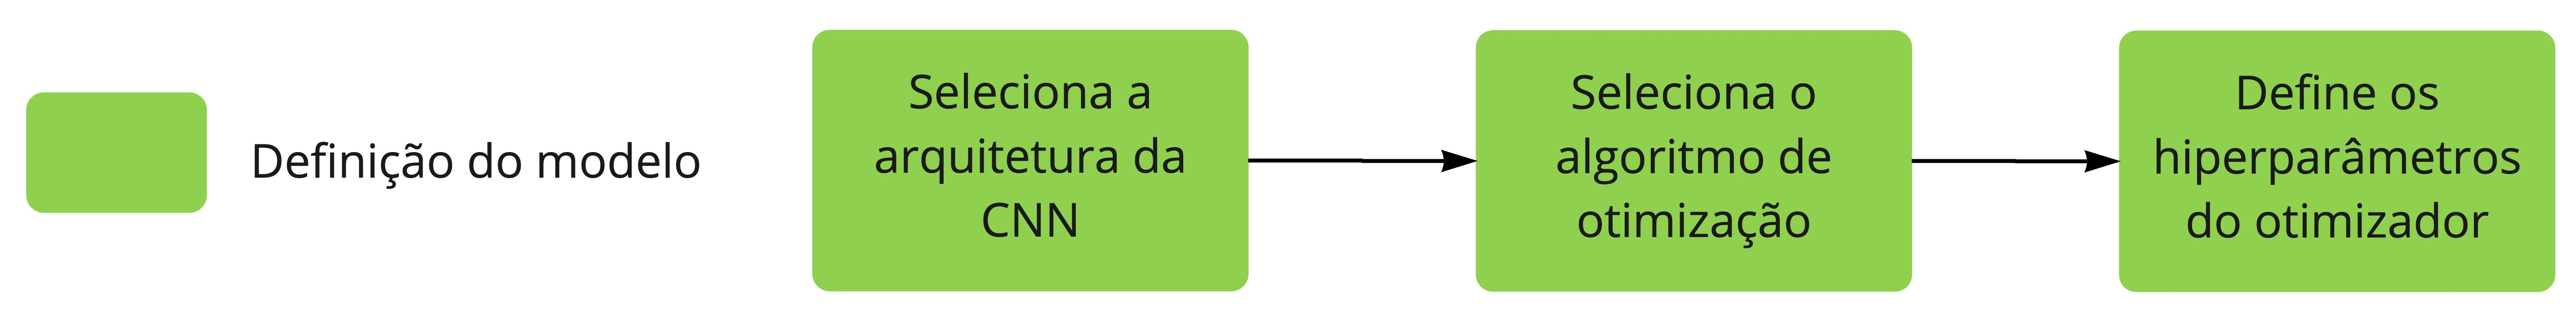
\includegraphics[width=1.0\textwidth]{imagens/materiais_metodos/modulo_modelo/pipeline_modelo_cnn_grupo_definicao_modelo.jpg}
    \label{fig:pipeline_modelo_cnn_grupo_definicao_modelo}
    \source{Danilo Assunção, 2022}
\end{figure}

\subsection{Grupo de treinamento e validação}
Este grupo possui as etapas responsáveis por realizar o fluxo de treinamento e validação do modelo utilizando os conjuntos de treinamento e validação para, respectivamente, obter e armazenar os resultados deste processamento e exibir algumas representações gráficas dos resultados retornados. O fluxo de todo o processo pode ser visto na Figura \ref{fig:pipeline_modelo_cnn_grupo_treinamento_validacao}.
                         
\begin{figure}[H]
    \centering
    \caption{Grupo de treinamento e validação}
    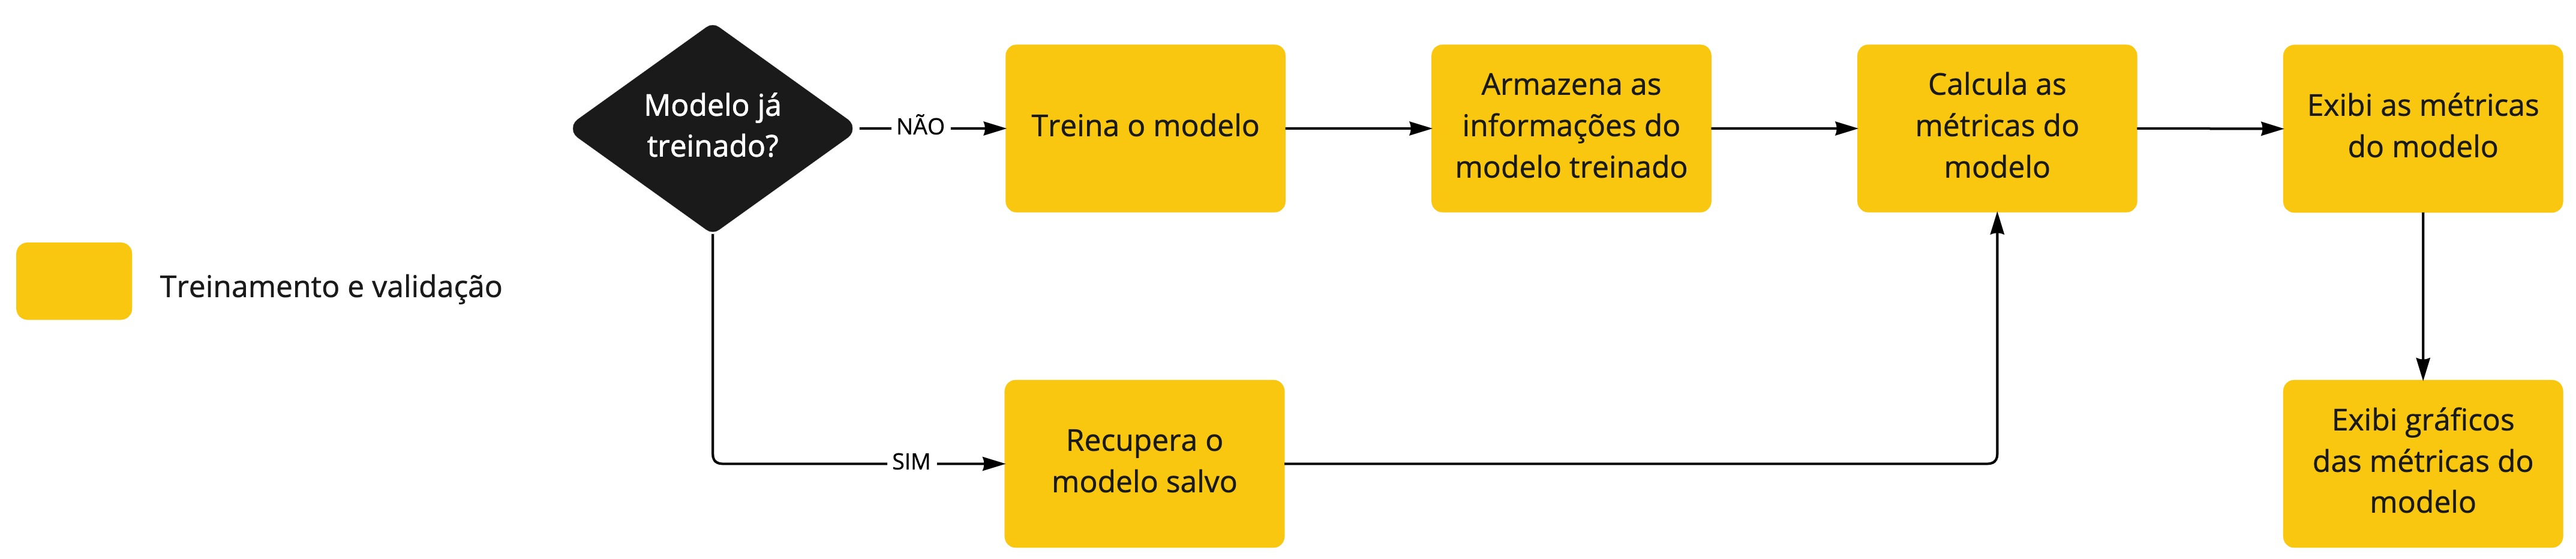
\includegraphics[width=1.0\textwidth]{imagens/materiais_metodos/modulo_modelo/pipeline_modelo_cnn_grupo_treinamento_validacao.jpg}
    \label{fig:pipeline_modelo_cnn_grupo_treinamento_validacao}
    \source{Danilo Assunção, 2022}
\end{figure}

O fluxo de treinamento e validação realiza uma checagem, na qual consiste em validar se as configurações definidas para o algoritmo do modelo selecionado já possui dados salvos de treinamento, caso houver, é feita a recuperação destes dados do modelo já treinado na nuvem, para assim seguir para o passo de cálculo e exibição das métricas do treinamento, caso contrário é realizado o treinamento do modelo e executado os passos seguintes. As métricas do processo de treinamento são exibidas durante cada época e, no final de todo o treinamento, é feita a coleta das medidas resultantes deste processo, sendo essas medidas a Precisão, Revocação, Acurácia e Taxa de erro. Com a visualização gráfica desses resultados, são geradas duas representações, sendo elas, o gráfico de acurácia por épocas e o gráfico de perda por épocas (dados da função de perda).

\subsection{Grupo de teste}
Neste grupo o modelo é testado utilizando o conjunto de dados de teste a partir do modelo treinado. Dado esta análise, logo em seguida é realizado o cálculo das medidas como Precisão, Revocação, Acurácia, Medida F e a Matriz Confusão. Por fim, estes resultados são armazenados em estruturas organizadas no \textit{Google Drive}. A representação do fluxo das etapas do grupo de teste pode ser visto através da Figura \ref{fig:pipeline_modelo_cnn_grupo_teste}.

\begin{figure}[H]
    \centering
    \caption{Grupo de teste}
    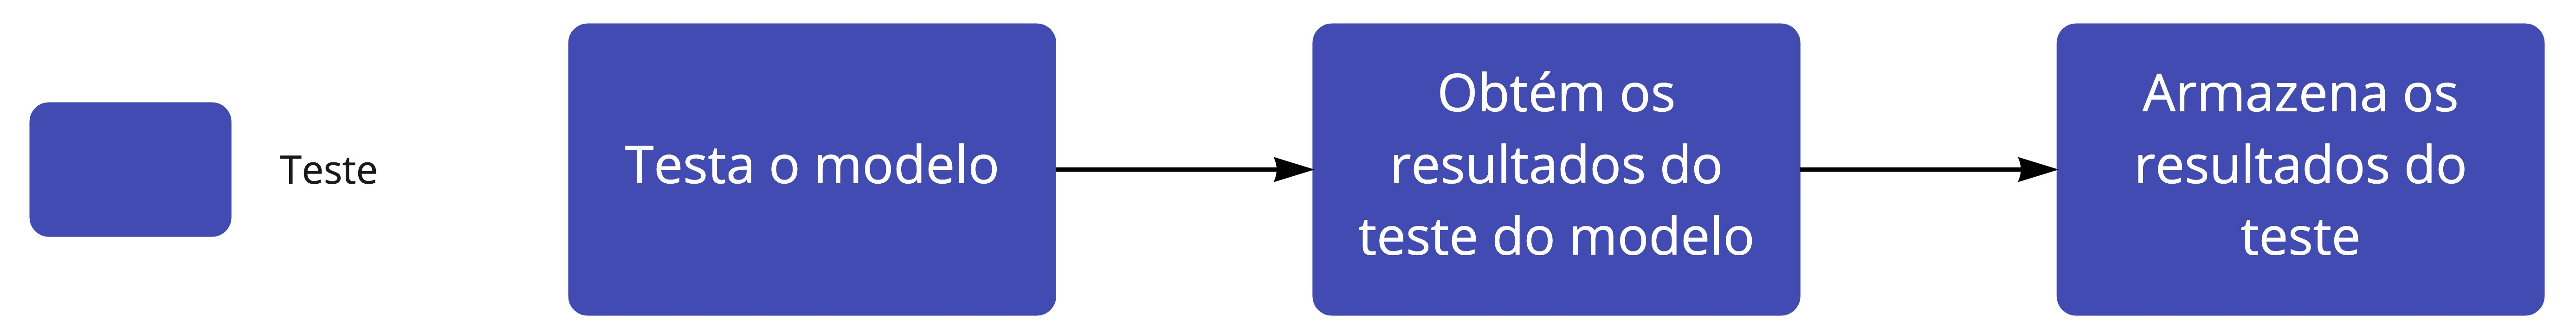
\includegraphics[width=1.0\textwidth]{imagens/materiais_metodos/modulo_modelo/pipeline_modelo_cnn_grupo_teste.jpg}
    \label{fig:pipeline_modelo_cnn_grupo_teste}
    \source{Danilo Assunção, 2022}
\end{figure}

\section{Avaliação}
\label{sec:avaliacao}
A avaliação consiste em comparar os resultados produzidos automaticamente pela CNN e, assim, observar a aplicação de métricas de aprendizado de máquina supervisionado (Revocação, Precisão, Acurácia, Medida F), possibilitando mensurar os resultados obtidos no processo de discriminação das classes, com o objetivo de obter o estado da arte para o modelo adequado ao problema proposto. A estratégia para esta avaliação será feita a partir de determinados passos, representados pela Figura \ref{fig:estrategia_experimentacao}.

\begin{figure}[H]
    \centering
    \caption{Estratégia de experimentação}
    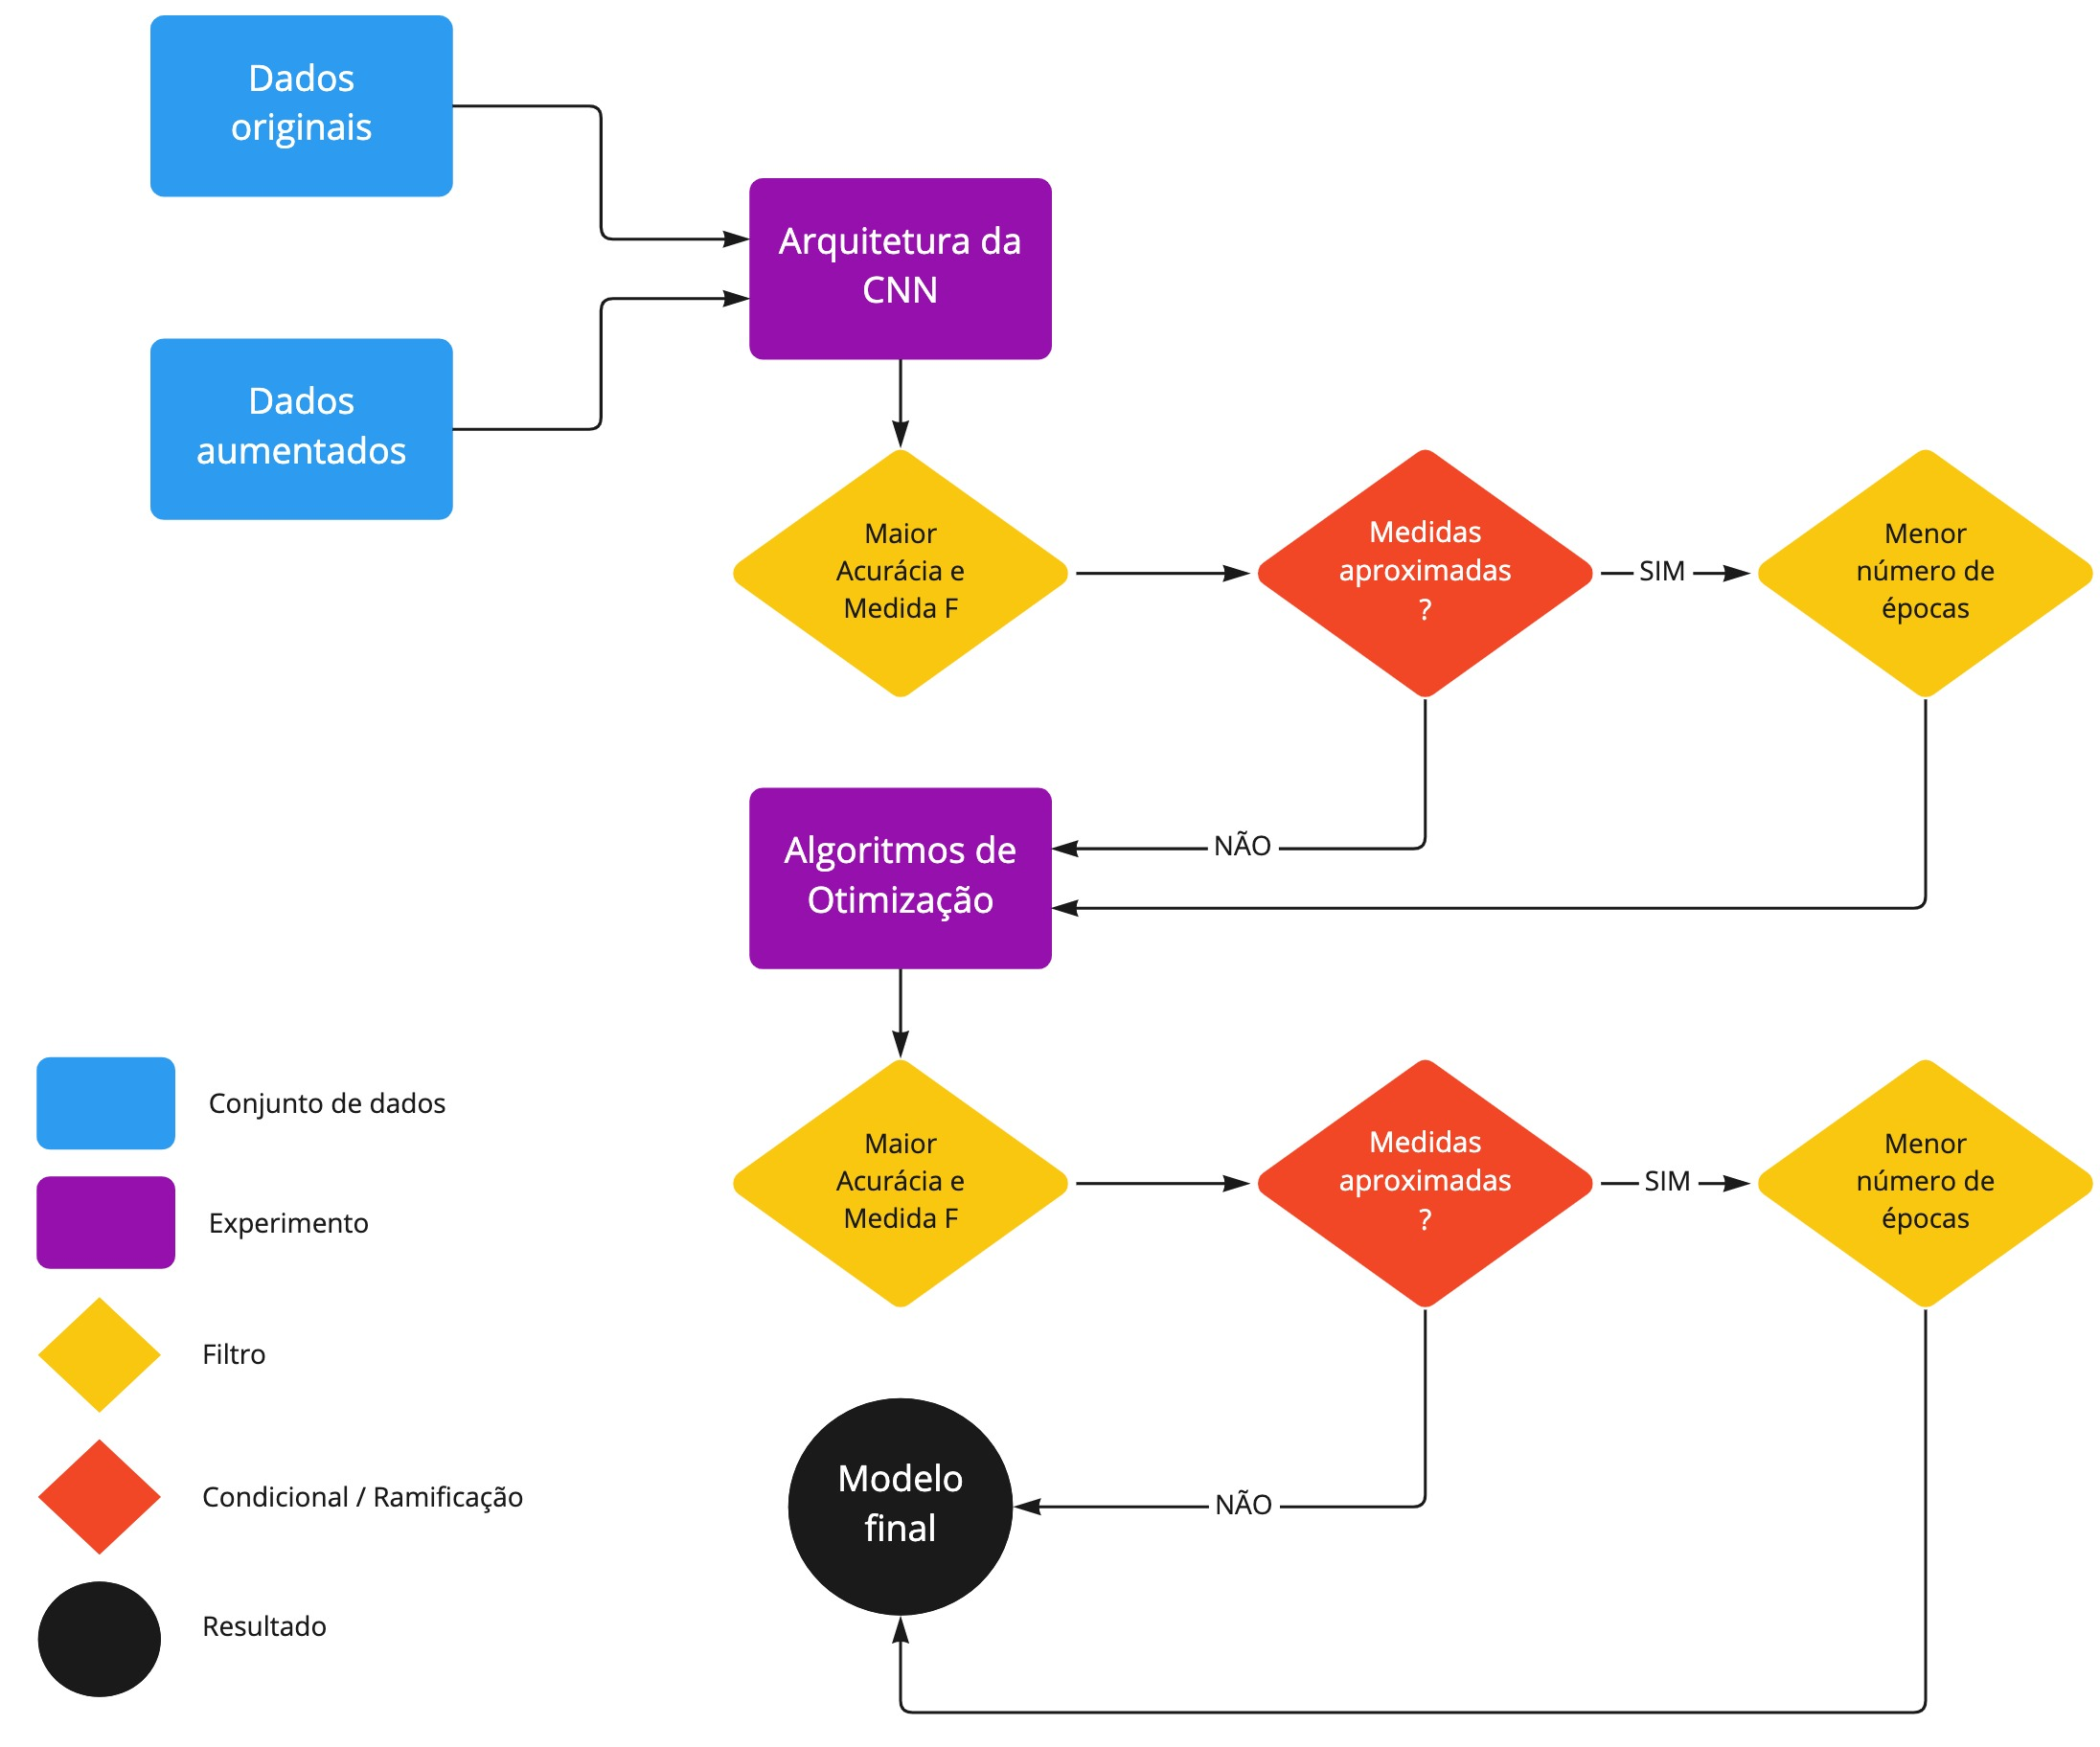
\includegraphics[scale=.18]{imagens/materiais_metodos/avaliacao/estrategia_experimentacao.jpg}
    \label{fig:estrategia_experimentacao}
    \source{Danilo Assunção, 2022}
\end{figure}

A estratégia de experimentação estabelecida é ilustrada na Figura \ref{fig:estrategia_experimentacao}, em que o processo realiza a seleção da arquitetura de CNN e do algoritmo de otimização para a CNN que demonstrar o melhor resultado, baseando-se no modelo abordado e seguindo as etapas pré-estabelecidas.

Serão utilizados dois conjuntos de dados para essa experimentação, sendo eles, o conjunto com as imagens originais e o conjunto com as imagens aumentadas pela técnica de aumento de dados. Para cada conjunto, foi feito a atribuição de etapas contendo uma experimentação que consiste na execução de um mecanismo que produz métricas de comparação, e um filtro que determina o item que será utilizado na próxima etapa do fluxo de experimentação. A primeira etapa consiste em determinar qual arquitetura de CNN será selecionada com base nas arquiteturas propostas, e, para todos estes exemplares propostos, foram considerados os hiperparâmetros relacionados em \citeonline{buschbacher2020image}. Com ênfase nas técnicas e experiências de tal trabalho, foi feito o uso de SGD como algoritmo de otimização com um valor de momento (técnica incluída no SGD que acumula o gradiente dos passos anteriores para determinar a direção a seguir) de 0,9 e com uma taxa de aprendizado de 0,001 para até 30 épocas, 0,0005 de 31 a 40 épocas e 0,0001 de 41 a 50 épocas, que será o número total de épocas aplicada nos experimentos, e, para as arquiteturas de CNN propostas, será feito um caso de teste com ou sem o uso de uma técnica de transferência de aprendizado. Após a realização das experimentações citadas anteriormente, os valores obtidos passaram por um filtro que determinará qual a arquitetura de CNN empregada no modelo que alcançou a maior Acurácia e Medida F. Durante o experimento de seleção da CNN, é considerada uma regra de captura destes resultados, realizando o armazenamento dos dados do modelo para uma determinada época, sendo isso apontado com base em uma condição de parada, que é acionada caso após as cinco épocas de treinamento seguintes do modelo não houver melhorias em seu desempenho. Após a execução deste primeiro experimento é feita uma validação e, assim, avaliar a existência de testes com resultados aproximados, dado este caso, será feito o uso de um segundo filtro, determinando a melhor arquitetura de CNN do modelo com base no número de épocas usado em treinamento para os modelos treinados nesta etapa.

Para a última etapa do experimento, foi considerada a escolha do algoritmo de otimização mais adequado para a arquitetura de CNN selecionada no passo anterior, em que serão realizados experimentos utilizando a arquitetura selecionada através do primeiro experimento, porém, realizado os testes a partir da utilização dos algoritmos de otimização propostos. A seleção do algoritmo de otimização foi definido ao filtrar o cenário que tiver como resultado a maior Acurácia e Medida F entre eles. Em adicional, caso existam cenários com resultados aproximados, foi considerado a aplicação de mais um filtro, considerando o número de épocas exigidas para se obter o melhor modelo deste experimento.

\begin{comment}
%------------------------------------------------------------------------
% CAPITULO - PROPOSTA DE PESQUISA
% Somente habilitado na qualificação
%------------------------------------------------------------------------
\chapter{Proposta de pesquisa}
Na literatura foi possível observar que, o processo de extração manual de características das imagens é algo fundamental para um melhor desempenho na classificação, mas é tida como uma tarefa especializada e trabalhosa. Muitas dessas características de mais alto nível acabam por não poder ser extraídas manualmente ao utilizar apenas métodos de segmentação. Sendo assim, um procedimento que permita determinar automaticamente as características adequadas para um deliberado problema, que envolva a identificação por meio de imagens vem sendo muito requisitado  \cite{waldchen2018machine}. No campo da ecologia, uma das tarefas é a identificação de espécies de abelhas a partir de imagens de suas asas \cite{liu2020classification}, visto que a combinação de técnicas que envolvem o mecanismo de aprendizado profundo não é normalmente explorado \cite{liu2020classification}. Entretanto, pesquisadores têm demonstrado, nos últimos anos, um aumento no interesse pela área de aprendizado de máquina, na qual a construção de sistemas de classificação de espécies mais eficientes, que utilizam técnicas de aprendizagem de máquina, acaba por ser de grande interesse e aplicabilidade no ramo científico \cite{liu2020classification}. Para a aplicação de uma CNN na resolução de problemas envolvendo imagens e reconhecimento de espécies, é necessária uma quantidade maior de dados para que a rede consiga convergir para um bom quadro de hipóteses, permitindo alcançar melhores resultados no processo de reconhecimento. Portanto, dois problemas ocorrem no treinamento destes modelos em conjunto de dados ecológicos, sendo eles o conjunto de dados de imagens limitado e os números de instâncias desequilibrados entre as diferentes classes, dessa maneira, as precisões dos modelos de CNN existentes para conjuntos de dados ecológicos podem ser baixas \cite{liu2020classification}. Visando a resolver os problemas mencionados, neste trabalho será utilizada uma CNN para, assim, realizar a extração automática das características contidas na morfologia das asas das abelhas presentes em imagens digitais. Baseando-se nas características obtidas para a identificação das respectivas espécies, em conjunto a técnicas de aumento de dados na série de imagens disponibilizadas que, serão ampliadas em diversas vezes os seus tamanhos, permitindo que o modelo possa treinar em um conjunto de dados maior com finalidade de obter-se melhores resultados através desse modelo, visando também a elevar a eficiência da velocidade de convergência do modelo a partir de técnicas de transferências de aprendizado. Almeja-se, assim, um melhor desempenho nos resultados para o processo de classificação das espécies de abelhas.

\section{Plano de trabalho e cronograma}
A seguir são apresentados um cronograma representado pela Tabela \ref{tab:cronograma} e todas as atividades que englobam este projeto de pesquisa:

\begin{enumerate}
  \item Revisão bibliográfica: uma revisão sistemática da literatura foi realizada propositando a identificar o estado da arte a partir de CNNs, utilizando técnicas que, provêem um mecanismo que permita o uso deste tipo de rede em diversos cenários para a identificação de espécies;
  \item Teste de proficiência em inglês: realização da prova de proficiência em inglês solicitada pelo programa;
  \item Qualificação: realização do exame de qualificação;
  \item Publicação de artigo: publicação de um artigo científico demonstrando os resultados obtidos no processo de identificação de espécies com o uso de CNNs;
  \item Preparação dos dados: criação de uma ferramenta responsável por executar diversos tratamentos em cima dos conjuntos de dados originais, para a criação e organização dos conjuntos de dados de treinamento, validação e teste;
  \item Preparação do modelo: criação de uma ferramenta para configuração e execução de modelos de aprendizado de máquina para diversas arquiteturas de CNNs;
  \item Execução do modelo: execução das ferramentas propostas, teste do modelo e armazenamento automático dos resultados obtidos na execução dos testes;
  \item Avaliação: testes utilizando os resultados obtidos na execução do modelo e análise dos resultados obtidos;
  \item Escrita da dissertação;
  \item Defesa.
\end{enumerate}

%----------------------------------------------------
% TABELA - CRONOGRAMA
%----------------------------------------------------
\begin{table}[H]
\centering
\caption{Cronograma}
\label{tab:cronograma}
\resizebox{\textwidth}{!}{%
\begin{tabular}{|ll|lllll|llllllllllll|llllllll|}
\hline
\multicolumn{2}{|l|}{Atividade} &
  \multicolumn{5}{l|}{2020} &
  \multicolumn{12}{l|}{2021} &
  \multicolumn{8}{l|}{2022} \\ \hline
\multicolumn{1}{|l|}{\#} &
  Descrição &
  \multicolumn{1}{l|}{8} &
  \multicolumn{1}{l|}{9} &
  \multicolumn{1}{l|}{10} &
  \multicolumn{1}{l|}{11} &
  12 &
  \multicolumn{1}{l|}{1} &
  \multicolumn{1}{l|}{2} &
  \multicolumn{1}{l|}{3} &
  \multicolumn{1}{l|}{4} &
  \multicolumn{1}{l|}{5} &
  \multicolumn{1}{l|}{6} &
  \multicolumn{1}{l|}{7} &
  \multicolumn{1}{l|}{8} &
  \multicolumn{1}{l|}{9} &
  \multicolumn{1}{l|}{10} &
  \multicolumn{1}{l|}{11} &
  12 &
  \multicolumn{1}{l|}{1} &
  \multicolumn{1}{l|}{2} &
  \multicolumn{1}{l|}{3} &
  \multicolumn{1}{l|}{4} &
  \multicolumn{1}{l|}{5} &
  \multicolumn{1}{l|}{6} &
  \multicolumn{1}{l|}{7} &
  8 \\ \hline
\multicolumn{1}{|l|}{1} &
  Revisão bibliográfica &
  \multicolumn{1}{l|}{x} &
  \multicolumn{1}{l|}{x} &
  \multicolumn{1}{l|}{x} &
  \multicolumn{1}{l|}{x} &
  x &
  \multicolumn{1}{l|}{x} &
  \multicolumn{1}{l|}{x} &
  \multicolumn{1}{l|}{x} &
  \multicolumn{1}{l|}{x} &
  \multicolumn{1}{l|}{} &
  \multicolumn{1}{l|}{} &
  \multicolumn{1}{l|}{} &
  \multicolumn{1}{l|}{} &
  \multicolumn{1}{l|}{} &
  \multicolumn{1}{l|}{} &
  \multicolumn{1}{l|}{} &
   &
  \multicolumn{1}{l|}{} &
  \multicolumn{1}{l|}{} &
  \multicolumn{1}{l|}{} &
  \multicolumn{1}{l|}{} &
  \multicolumn{1}{l|}{} &
  \multicolumn{1}{l|}{} &
  \multicolumn{1}{l|}{} &
   \\ \hline
\multicolumn{1}{|l|}{2} &
  Teste de proficiencia em inglês &
  \multicolumn{1}{l|}{} &
  \multicolumn{1}{l|}{} &
  \multicolumn{1}{l|}{} &
  \multicolumn{1}{l|}{} &
   &
  \multicolumn{1}{l|}{} &
  \multicolumn{1}{l|}{} &
  \multicolumn{1}{l|}{} &
  \multicolumn{1}{l|}{} &
  \multicolumn{1}{l|}{x} &
  \multicolumn{1}{l|}{} &
  \multicolumn{1}{l|}{} &
  \multicolumn{1}{l|}{} &
  \multicolumn{1}{l|}{} &
  \multicolumn{1}{l|}{} &
  \multicolumn{1}{l|}{} &
   &
  \multicolumn{1}{l|}{} &
  \multicolumn{1}{l|}{} &
  \multicolumn{1}{l|}{} &
  \multicolumn{1}{l|}{} &
  \multicolumn{1}{l|}{} &
  \multicolumn{1}{l|}{} &
  \multicolumn{1}{l|}{} &
   \\ \hline
\multicolumn{1}{|l|}{3} &
  Qualificação &
  \multicolumn{1}{l|}{} &
  \multicolumn{1}{l|}{} &
  \multicolumn{1}{l|}{} &
  \multicolumn{1}{l|}{} &
   &
  \multicolumn{1}{l|}{} &
  \multicolumn{1}{l|}{} &
  \multicolumn{1}{l|}{} &
  \multicolumn{1}{l|}{} &
  \multicolumn{1}{l|}{} &
  \multicolumn{1}{l|}{x} &
  \multicolumn{1}{l|}{} &
  \multicolumn{1}{l|}{} &
  \multicolumn{1}{l|}{} &
  \multicolumn{1}{l|}{} &
  \multicolumn{1}{l|}{} &
   &
  \multicolumn{1}{l|}{} &
  \multicolumn{1}{l|}{} &
  \multicolumn{1}{l|}{} &
  \multicolumn{1}{l|}{} &
  \multicolumn{1}{l|}{} &
  \multicolumn{1}{l|}{} &
  \multicolumn{1}{l|}{} &
   \\ \hline
\multicolumn{1}{|l|}{4} &
  Publicação de artigo &
  \multicolumn{1}{l|}{} &
  \multicolumn{1}{l|}{} &
  \multicolumn{1}{l|}{} &
  \multicolumn{1}{l|}{} &
   &
  \multicolumn{1}{l|}{} &
  \multicolumn{1}{l|}{} &
  \multicolumn{1}{l|}{} &
  \multicolumn{1}{l|}{} &
  \multicolumn{1}{l|}{} &
  \multicolumn{1}{l|}{} &
  \multicolumn{1}{l|}{} &
  \multicolumn{1}{l|}{} &
  \multicolumn{1}{l|}{} &
  \multicolumn{1}{l|}{} &
  \multicolumn{1}{l|}{x} &
  x &
  \multicolumn{1}{l|}{x} &
  \multicolumn{1}{l|}{} &
  \multicolumn{1}{l|}{} &
  \multicolumn{1}{l|}{} &
  \multicolumn{1}{l|}{} &
  \multicolumn{1}{l|}{} &
  \multicolumn{1}{l|}{x} &
  x \\ \hline
\multicolumn{1}{|l|}{5} &
  Preparação dos dados &
  \multicolumn{1}{l|}{} &
  \multicolumn{1}{l|}{} &
  \multicolumn{1}{l|}{} &
  \multicolumn{1}{l|}{} &
   &
  \multicolumn{1}{l|}{} &
  \multicolumn{1}{l|}{} &
  \multicolumn{1}{l|}{} &
  \multicolumn{1}{l|}{} &
  \multicolumn{1}{l|}{x} &
  \multicolumn{1}{l|}{x} &
  \multicolumn{1}{l|}{x} &
  \multicolumn{1}{l|}{x} &
  \multicolumn{1}{l|}{x} &
  \multicolumn{1}{l|}{x} &
  \multicolumn{1}{l|}{x} &
  x &
  \multicolumn{1}{l|}{} &
  \multicolumn{1}{l|}{} &
  \multicolumn{1}{l|}{} &
  \multicolumn{1}{l|}{} &
  \multicolumn{1}{l|}{} &
  \multicolumn{1}{l|}{} &
  \multicolumn{1}{l|}{} &
   \\ \hline
\multicolumn{1}{|l|}{6} &
  Preparação do modelo &
  \multicolumn{1}{l|}{} &
  \multicolumn{1}{l|}{} &
  \multicolumn{1}{l|}{} &
  \multicolumn{1}{l|}{} &
   &
  \multicolumn{1}{l|}{} &
  \multicolumn{1}{l|}{} &
  \multicolumn{1}{l|}{} &
  \multicolumn{1}{l|}{} &
  \multicolumn{1}{l|}{} &
  \multicolumn{1}{l|}{x} &
  \multicolumn{1}{l|}{x} &
  \multicolumn{1}{l|}{x} &
  \multicolumn{1}{l|}{x} &
  \multicolumn{1}{l|}{x} &
  \multicolumn{1}{l|}{x} &
  x &
  \multicolumn{1}{l|}{x} &
  \multicolumn{1}{l|}{} &
  \multicolumn{1}{l|}{} &
  \multicolumn{1}{l|}{} &
  \multicolumn{1}{l|}{} &
  \multicolumn{1}{l|}{} &
  \multicolumn{1}{l|}{} &
   \\ \hline
\multicolumn{1}{|l|}{7} &
  Execução do modelo &
  \multicolumn{1}{l|}{} &
  \multicolumn{1}{l|}{} &
  \multicolumn{1}{l|}{} &
  \multicolumn{1}{l|}{} &
   &
  \multicolumn{1}{l|}{} &
  \multicolumn{1}{l|}{} &
  \multicolumn{1}{l|}{} &
  \multicolumn{1}{l|}{} &
  \multicolumn{1}{l|}{} &
  \multicolumn{1}{l|}{} &
  \multicolumn{1}{l|}{} &
  \multicolumn{1}{l|}{} &
  \multicolumn{1}{l|}{x} &
  \multicolumn{1}{l|}{x} &
  \multicolumn{1}{l|}{x} &
  x &
  \multicolumn{1}{l|}{x} &
  \multicolumn{1}{l|}{x} &
  \multicolumn{1}{l|}{x} &
  \multicolumn{1}{l|}{x} &
  \multicolumn{1}{l|}{} &
  \multicolumn{1}{l|}{} &
  \multicolumn{1}{l|}{} &
   \\ \hline
\multicolumn{1}{|l|}{8} &
  Avaliação &
  \multicolumn{1}{l|}{} &
  \multicolumn{1}{l|}{} &
  \multicolumn{1}{l|}{} &
  \multicolumn{1}{l|}{} &
   &
  \multicolumn{1}{l|}{} &
  \multicolumn{1}{l|}{} &
  \multicolumn{1}{l|}{} &
  \multicolumn{1}{l|}{} &
  \multicolumn{1}{l|}{} &
  \multicolumn{1}{l|}{} &
  \multicolumn{1}{l|}{} &
  \multicolumn{1}{l|}{} &
  \multicolumn{1}{l|}{} &
  \multicolumn{1}{l|}{} &
  \multicolumn{1}{l|}{} &
   &
  \multicolumn{1}{l|}{} &
  \multicolumn{1}{l|}{} &
  \multicolumn{1}{l|}{x} &
  \multicolumn{1}{l|}{x} &
  \multicolumn{1}{l|}{x} &
  \multicolumn{1}{l|}{x} &
  \multicolumn{1}{l|}{} &
   \\ \hline
\multicolumn{1}{|l|}{9} &
  Texto de dissertação &
  \multicolumn{1}{l|}{} &
  \multicolumn{1}{l|}{} &
  \multicolumn{1}{l|}{} &
  \multicolumn{1}{l|}{} &
   &
  \multicolumn{1}{l|}{} &
  \multicolumn{1}{l|}{} &
  \multicolumn{1}{l|}{} &
  \multicolumn{1}{l|}{} &
  \multicolumn{1}{l|}{} &
  \multicolumn{1}{l|}{} &
  \multicolumn{1}{l|}{} &
  \multicolumn{1}{l|}{} &
  \multicolumn{1}{l|}{} &
  \multicolumn{1}{l|}{} &
  \multicolumn{1}{l|}{} &
   &
  \multicolumn{1}{l|}{x} &
  \multicolumn{1}{l|}{x} &
  \multicolumn{1}{l|}{x} &
  \multicolumn{1}{l|}{x} &
  \multicolumn{1}{l|}{x} &
  \multicolumn{1}{l|}{x} &
  \multicolumn{1}{l|}{x} &
  x \\ \hline
\multicolumn{1}{|l|}{10} &
  Defesa &
  \multicolumn{1}{l|}{} &
  \multicolumn{1}{l|}{} &
  \multicolumn{1}{l|}{} &
  \multicolumn{1}{l|}{} &
   &
  \multicolumn{1}{l|}{} &
  \multicolumn{1}{l|}{} &
  \multicolumn{1}{l|}{} &
  \multicolumn{1}{l|}{} &
  \multicolumn{1}{l|}{} &
  \multicolumn{1}{l|}{} &
  \multicolumn{1}{l|}{} &
  \multicolumn{1}{l|}{} &
  \multicolumn{1}{l|}{} &
  \multicolumn{1}{l|}{} &
  \multicolumn{1}{l|}{} &
   &
  \multicolumn{1}{l|}{} &
  \multicolumn{1}{l|}{} &
  \multicolumn{1}{l|}{} &
  \multicolumn{1}{l|}{} &
  \multicolumn{1}{l|}{} &
  \multicolumn{1}{l|}{} &
  \multicolumn{1}{l|}{} &
  x \\ \hline
\end{tabular}%
}
\source{Danilo Assunção, 2022}
\end{table}

\section{Considerações finais}
Este trabalho propõe a utilização de visão computacional para a construção de um modelo de CNN, o qual realiza o reconhecimento de espécies de abelhas a partir da morfologia de suas asas presentes em imagens digitais. Pretende-se utilizar em conjunto a este mecanismo, técnicas de aumento de dados e transferência de aprendizado. Inicialmente, foi realizada uma revisão sistemática da literatura, que identificou as técnicas de aumento de dados e transferência de aprendizado utilizando algoritmos de CNN para tarefas de reconhecimento de espécies no geral. Esta revisão permitiu o entendimento das diversas possibilidades disponíveis para a aplicação de técnicas de aprendizado profundo, mesmo quando se tem poucos dados disponíveis, o que permite uma maior autonomia e flexibilidade no acolhimento das características das imagens, junto a uma automatização como um todo no processo de reconhecimento. Com este método, espera-se obter bons resultados na classificação das espécies de abelhas, utilizando um modelo de CNN como automatizador de todo o processo de extração e classificação deste domínio.
\end{comment}

%------------------------------------------------------------------------
% CAPITULO - Resultados e discussões
%------------------------------------------------------------------------
\chapter{Resultados e discussões}
Este capítulo detalha os resultados obtidos durante o processo de treinamento, validação e teste do modelo de aprendizado de máquina utilizando algoritmos de CNN e otimização que foram selecionados para a resolução do problema em questão, que envolve a identificação automática de espécies de abelhas através de imagens de suas asas.

Seguindo as diretrizes estabelecidas pela metodologia especificada, é feito o detalhamento dos resultados e a exemplificação de cada cenário de maneira descritiva e ilustrativa a partir dos dados coletados nesta etapa. Dito isto, as seções a seguir seguirão o detalhamento dos passos descritos pela Figura \ref{fig:estrategia_experimentacao}, considerando as etapas de experimentação, em que é sucedida a primeira etapa para seleção da arquitetura de CNN, e, por fim, a seleção do algoritmo de otimização para a CNN.

\section{Seleção da arquitetura da CNN}
Esta seção tem como objetivo, detalhar os experimentos realizados no processo de seleção da arquitetura da CNN que obteve o melhor resultado com relação ao domínio proposto. As arquiteturas de CNN abordadas neste trabalho foram selecionadas com base na revisão sistemática feita também neste trabalho, sendo elas, InceptionResNet v2, Inception v3, ResNet-152, VGG16 e VGG19. Tais arquiteturas também foram empregadas levando em consideração o uso de técnicas de aumento de dados e transferência de aprendizado para fins comparativos.

\subsection{InceptionResNet v2}
Para o modelo empregando a arquitetura de CNN InceptionResNet v2, o primeiro experimento realizado foi utilizando o conjunto de dados original, que contém as imagens disponibilizadas sem o uso de técnicas de aumento de dados. Este modelo foi treinado por até 34 épocas, posteriormente, não houve melhorias em seus resultados, considerando o critério de parada que são 5 épocas no total. Para os experimentos utilizando apenas InceptionResNet v2, não foi aplicada nenhuma técnica de transferência de aprendizado. A seguir, é possível visualizar os resultados obtidos na fase de treinamento para este experimento, através da Figura \ref{fig:inception_resnet_v2_dados_originais}.

\begin{figure}[H]
    \centering
    \caption{Resultados do treinamento com a InceptionResNet v2 + Dados originais}
    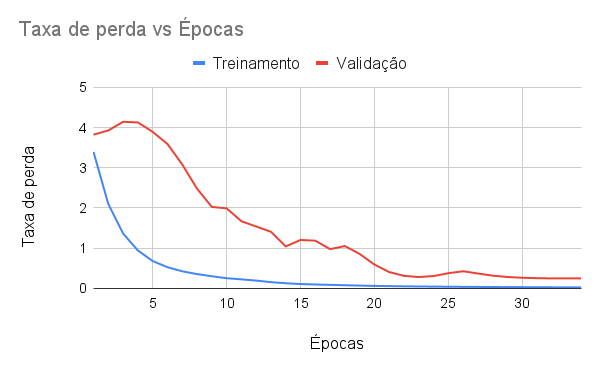
\includegraphics[width=.50\textwidth]{imagens/resultados_discussao/architecture/inception_resnet_v2/original/perda.png}\hfill
    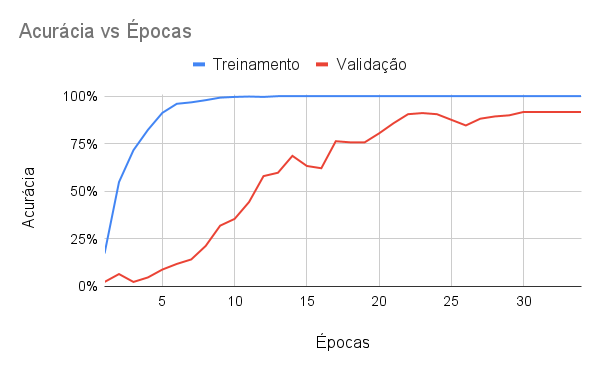
\includegraphics[width=.50\textwidth]{imagens/resultados_discussao/architecture/inception_resnet_v2/original/acuracia.png}\bigbreak    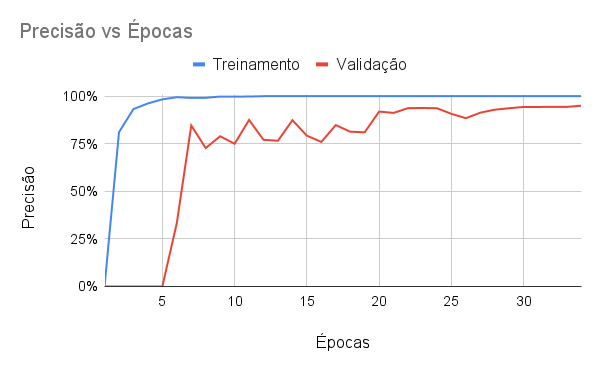
\includegraphics[width=.50\textwidth]{imagens/resultados_discussao/architecture/inception_resnet_v2/original/precisao.png}\hfill
    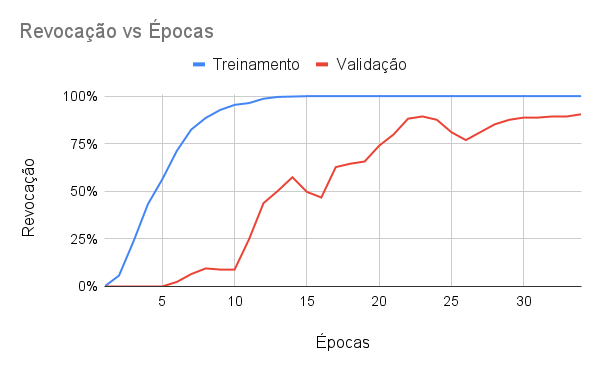
\includegraphics[width=.50\textwidth]{imagens/resultados_discussao/architecture/inception_resnet_v2/original/revocacao.png}
    \label{fig:inception_resnet_v2_dados_originais}
    \source{Danilo Assunção, 2022}
\end{figure}

As representações da Figura \ref{fig:inception_resnet_v2_dados_originais} representam as linhas de treinamento, que correspondem aos dados de treinamento obtidos em cada época do modelo e respectivamente a linha que representa os dados obtidos em cada época na validação do modelo e todos os gráficos representam, cada um deles, uma medida obtida para determinar o desempenho geral do modelo, sendo eles, respectivamente, a taxa de perda, acurácia, precisão e revocação resultantes deste processo. A taxa de perda é um número que mensura o fator de previsibilidade do modelo, ou seja, caso a previsão do modelo for boa, a perda tende à zero, caso contrário, a perda será maior.

Esta arquitetura é a união de duas arquiteturas consistentes que são a Inception e a ResNet, e, esta junção, visa a obter algumas características relevantes de ambas as arquiteturas, isto é, a família de arquiteturas Inception são exemplares que demonstram alcançar um desempenho muito bom a um custo computacional relativamente baixo \cite{szegedy2017inception}, enquanto a arquiteturas da família ResNet é uma abordagem que faz uso de conexões de atalho, e este aspecto auxilia na resolução do problema de Dissipação do Gradiente \cite{feng2017overview}, apontando que, no decorrer do treinamento de uma rede, os gradientes propagados passarão por multiplicações com valores menores que 1, realizados em cada camada da rede e possuindo valores mínimos ao chegar nas camadas inciais da rede. Tendo como efeito, o encontro também de valores mínimos pelo ajuste dos pesos, sendo ele calculado a cada iteração do treinamento da rede. Desta forma, devido ao requisito de uma elevada quantidade de iterações para se obter um ajuste minimamente considerável, acaba por acarretar em um alto custo para o treinamento das primeiras camadas da rede \cite{hochreiter1998vanishing}. Diante disso, a Dissipação do Gradiente soluciona problemas relacionados quando se possui redes muito profundas, dado que, a adição de mais camadas na rede permite determinar representações mais complexas e, para problemas mais complexos, possuir uma CNN profunda pode ser necessário. Para este modelo, foram obtidos os resultados e coletadas as suas medidas, sendo elas apresentadas no Quadro \ref{quad:resultados_teste_inception_resnet_v2_com_dados_originais}.

\begin{quadro}[H]
\caption{Resultados do teste com a InceptionResNet v2 + Dados originais}
\label{quad:resultados_teste_inception_resnet_v2_com_dados_originais}
\centering
\begin{tabular}{|l|l|l|l|l|l|l|l|}
\cline{1-8}
Épocas & Perda & Acurácia & Precisão & Revocação & Medida F & Acertos & Erros \\ \hline
34 & 0,24 & 90,58\% & 93,30\% & 87,43\% & 90,27\% & 173 & 18 \\
\cline{1-8}
\end{tabular}
\source{Danilo Assunção, 2022}
\end{quadro}

No teste deste experimento foi alcançado um valor de 90,27\% para a Medida F, que é a medida sendo utilizada para comparativo neste trabalho e, considerando que este modelo não possui nenhuma técnica de aumento de dados e transferência de aprendizado, ele conseguiu atingir um valor de 90,58\% de Acurácia, acertando um total de 173 imagens e errando 18 imagens.

Ainda visando melhorias no modelo atual, foi efetuada uma experimentação utilizando a mesma arquitetura de CNN, mas aplicando em adicional a técnica de aumento de dados ao conjunto de dados original, obtendo-se assim um conjunto de dados aumentado em até 7 vezes o seu tamanho original. Neste experimento, considerando o conjunto de dados aumentado, o modelo teve de treinar durante um total de 26 épocas, até não demonstrar mais melhorias e aplicar o critério de parada do processo de treinamento. Os dados adquiridos no treinamento deste modelo podem ser vistos na Figura \ref{fig:inception_resnet_v2_dados_aumentados}.

\begin{figure}[H]
    \centering
    \caption{Resultados do treinamento da InceptionResNet v2 + Dados aumentados}
    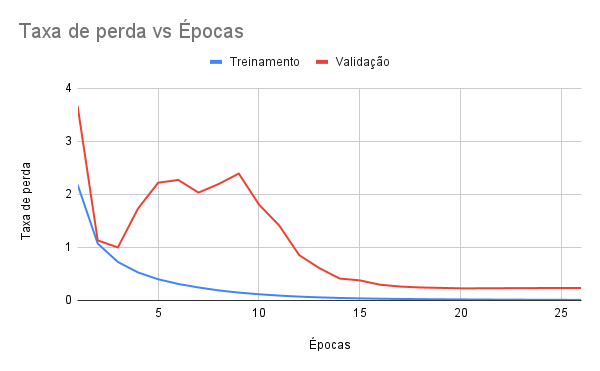
\includegraphics[width=.50\textwidth]{imagens/resultados_discussao/architecture/inception_resnet_v2/augmented/perda.png}\hfill
    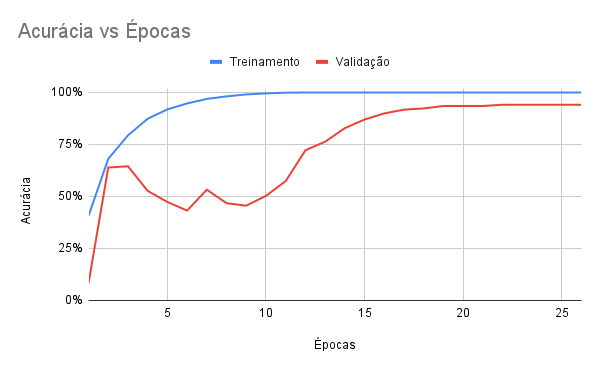
\includegraphics[width=.50\textwidth]{imagens/resultados_discussao/architecture/inception_resnet_v2/augmented/acuracia.png}\bigbreak    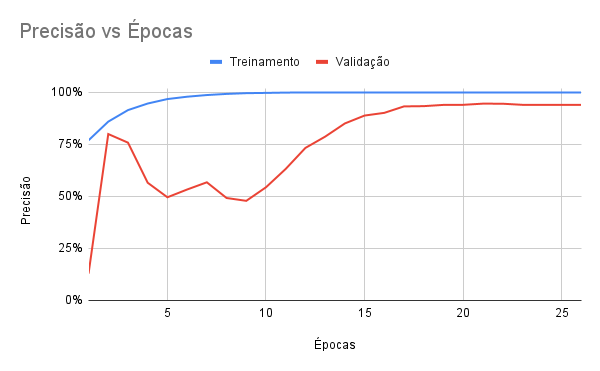
\includegraphics[width=.50\textwidth]{imagens/resultados_discussao/architecture/inception_resnet_v2/augmented/precisao.png}\hfill
    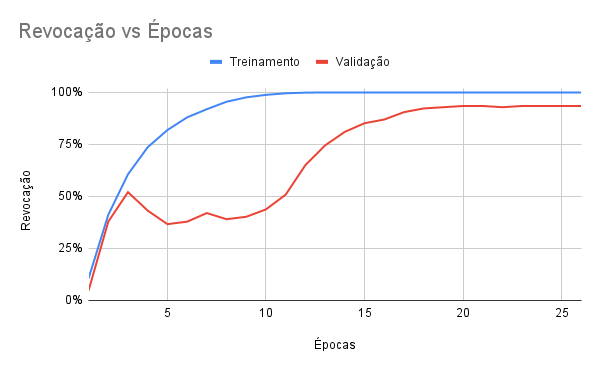
\includegraphics[width=.50\textwidth]{imagens/resultados_discussao/architecture/inception_resnet_v2/augmented/revocacao.png}
    \label{fig:inception_resnet_v2_dados_aumentados}
    \source{Danilo Assunção, 2022}
\end{figure}

Para a fase de teste deste modelo utilizando os dados aumentados, temos a visualização dos resultados obtidos no Quadro \ref{quad:resultados_teste_inception_resnet_v2_com_dados_aumentados}.

\begin{quadro}[H]
\caption{Resultados do teste com a InceptionResNet v2 + Dados aumentados}
\label{quad:resultados_teste_inception_resnet_v2_com_dados_aumentados}
\centering
\begin{tabular}{|l|l|l|l|l|l|l|l|}
\cline{1-8}
Épocas & Perda & Acurácia & Precisão & Revocação & Medida F & Acertos & Erros \\ \hline
26 & 0,13 & 94,24\% & 95,21\% & 93,72\% & 94,46\% & 180 & 11 \\
\cline{1-8}
\end{tabular}
\source{Danilo Assunção, 2022}
\end{quadro}

Comparando a Medida F e a Acurácia resultante dos dois últimos testes, o modelo que utilizou o conjunto de dados aumentado teve um acréscimo de 4,19\% em sua Medida F e 3,66\% em sua Acurácia, somente ampliando a quantidade de imagens do conjunto de dados. É observável também que, além do desempenho ter sido melhorado com o aumento de dados, a quantidade de épocas necessárias para se ter este resultado foi menor com relação ao modelo que não usa o aumento de dados, tendo utilizado 8 épocas a menos para se atingir resultados melhores neste modelo. Sendo assim, o uso da InceptionResNet v2 com aumento de dados, mostrou ser melhor neste experimento.

Considerando os modelos anteriores, foram também executados testes utilizando o conjunto de dados original e o conjunto de dados aumentado, junto à técnica de transferência de aprendizado. O primeiro teste foi feito empregando apenas o conjunto de dados original e seus dados obtidos no processo de treinamento, podendo ser observado na Figura \ref{fig:inception_resnet_v2_original_transferencia_aprendizado}.

\begin{figure}[H]
    \centering
    \caption{Resultados do treinamento com a InceptionResNet v2 + Dados originais + Transferência de aprendizado}
    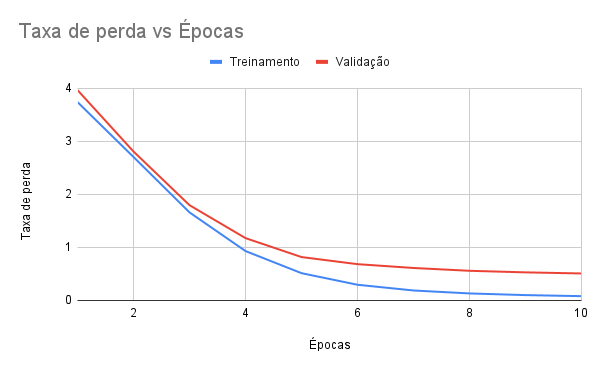
\includegraphics[width=.50\textwidth]{imagens/resultados_discussao/architecture/inception_resnet_v2/transfer_learning/original/perda.png}\hfill
    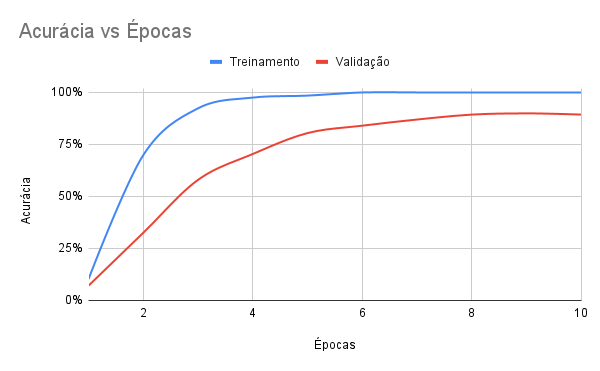
\includegraphics[width=.50\textwidth]{imagens/resultados_discussao/architecture/inception_resnet_v2/transfer_learning/original/acuracia.png}\bigbreak    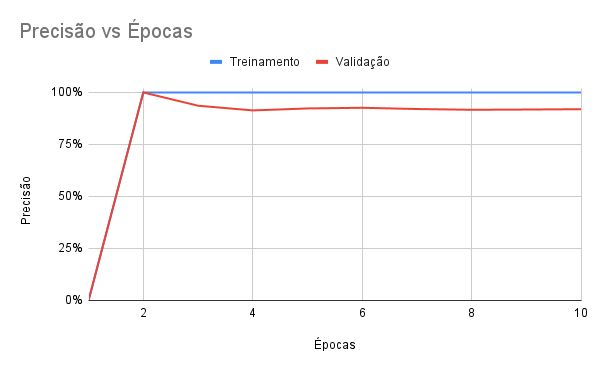
\includegraphics[width=.50\textwidth]{imagens/resultados_discussao/architecture/inception_resnet_v2/transfer_learning/original/precisao.png}\hfill
    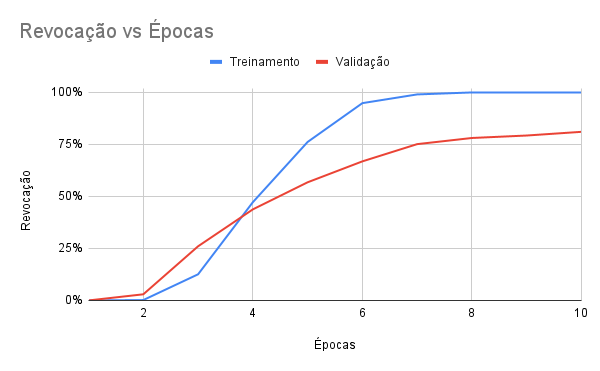
\includegraphics[width=.50\textwidth]{imagens/resultados_discussao/architecture/inception_resnet_v2/transfer_learning/original/revocacao.png}
    \label{fig:inception_resnet_v2_original_transferencia_aprendizado}
    \source{Danilo Assunção, 2022}
\end{figure}

Para o teste deste modelo foi coletado os valores que podem ser vistos através do Quadro \ref{quad:test_inception_resnet_v2_original_transfer_learning}.

\begin{quadro}[H]
\caption{Resultados do teste com a InceptionResNet v2 + Dados originais + Transferência de aprendizado}
\label{quad:test_inception_resnet_v2_original_transfer_learning}
\centering
\begin{tabular}{|l|l|l|l|l|l|l|l|}
\cline{1-8}
Épocas & Perda & Acurácia & Precisão & Revocação & Medida F & Acertos & Erros \\ \hline
10 & 0,47 & 90,58\% & 93,90\% & 80,63\% & 86,76\% & 173 & 18 \\
\cline{1-8}
\end{tabular}
\source{Danilo Assunção, 2022}
\end{quadro}

Por fim, o último experimento utilizando esta arquitetura foi feito aplicando ambas as técnicas de aumento de dados e de transferência de aprendizado. Os resultados obtidos durante o treinamento deste modelo, usando ambas as técnicas, podem ser analisados através da Figura \ref{fig:inception_resnet_v2_augmented_transfer_learning}.

\begin{figure}[H]
    \centering
    \caption{Resultados do treinamento com a InceptionResNet v2 + Dados aumentados + Transferência de aprendizado}
    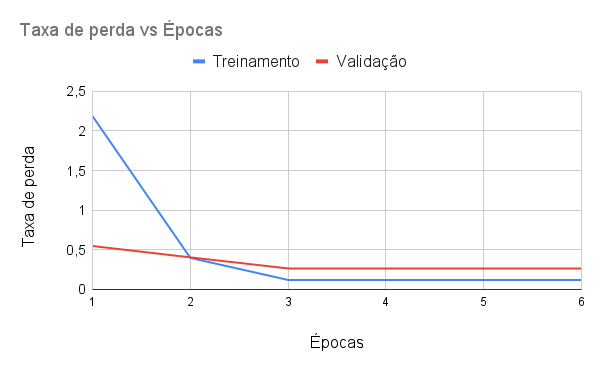
\includegraphics[width=.50\textwidth]{imagens/resultados_discussao/architecture/inception_resnet_v2/transfer_learning/augmented/perda.png}\hfill
    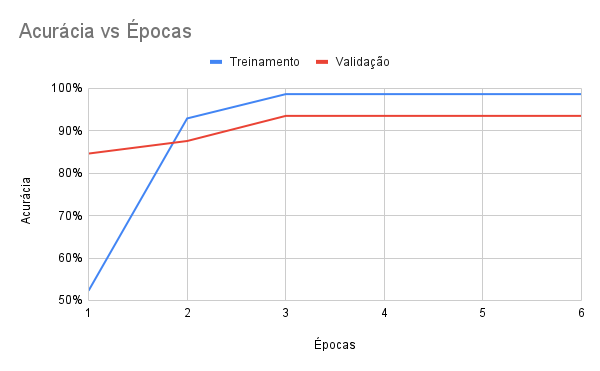
\includegraphics[width=.50\textwidth]{imagens/resultados_discussao/architecture/inception_resnet_v2/transfer_learning/augmented/acuracia.png}\bigbreak    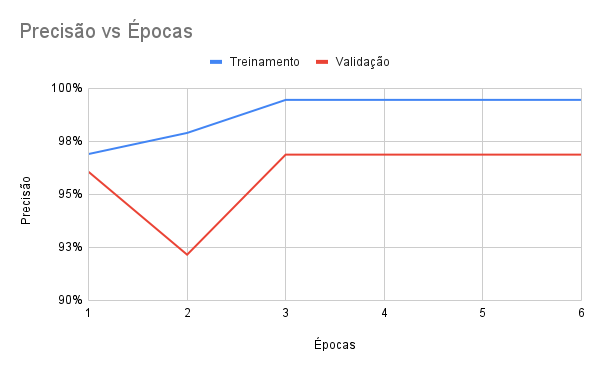
\includegraphics[width=.50\textwidth]{imagens/resultados_discussao/architecture/inception_resnet_v2/transfer_learning/augmented/precisao.png}\hfill
    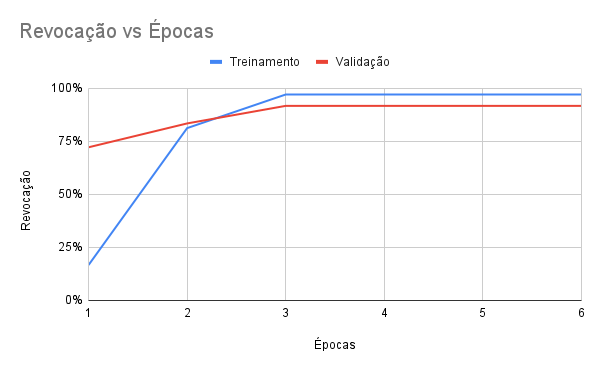
\includegraphics[width=.50\textwidth]{imagens/resultados_discussao/architecture/inception_resnet_v2/transfer_learning/augmented/revocacao.png}
    \label{fig:inception_resnet_v2_augmented_transfer_learning}
    \source{Danilo Assunção, 2022}
\end{figure}

O treinamento deste modelo, logo nas épocas iniciais, já demonstrava relativamente bons resultados devido ao uso da técnica de transferência de aprendizado. Em relação ao modelo que usa transferência de aprendizado com os dados originais, este exemplo precisou de apenas 6 épocas, tendo obtido seu melhor resultado em 4 épocas a menos em comparação com o modelo anterior. Os dados do teste deste experimento podem ser visualizados no Quadro \ref{quad:test_inception_resnet_v2_augmented_transfer_learning}.

\begin{quadro}[H]
\caption{Resultados do teste com a InceptionResNet v2 + Dados aumentados + Transferência de aprendizado}
\label{quad:test_inception_resnet_v2_augmented_transfer_learning}
\centering
\begin{tabular}{|l|l|l|l|l|l|l|l|}
\cline{1-8}
Épocas & Perda & Acurácia & Precisão & Revocação & Medida F & Acertos & Erros \\ \hline
5 & 0,31 & 91,62\% & 95,58\% & 90,58\% & 93,01\% & 175 & 16 \\
\cline{1-8}
\end{tabular}
\source{Danilo Assunção, 2022}
\end{quadro}

Os resultados em termos de desempenho deste último modelo, demonstraram melhores medidas em comparação com a Medida F e Acurácia do modelo que usa a técnica de transferência de aprendizado com o conjunto de dados original, tendo obtido uma melhoria de 6,25\% em sua Medida F e 1,04\% na Acurácia utilizando 5 épocas a menos do que o modelo anterior. 

Comparando os dois experimentos com maiores resultados, sendo eles, este último experimento e o experimento que utiliza apenas o conjunto de dados aumentado, em que, o experimento que aplica somente a técnica de aumento de dados foi superior a este último modelo experimentado, atingindo uma diferença de 1,45\% em sua Medida F e 2,62\% em sua Acurácia, entretanto utilizando 21 épocas a mais do que o modelo comparado.

\subsection{Inception v3}
Inception v3 é uma arquitetura de rede neural convolucional da família Inception que possui certas melhorias com relação a suas versões antecessoras, e foi construída com base em \citeonline{szegedy2016rethinking}. Para o modelo que usa a arquitetura Inception v3, na realização do primeiro experimento foi utilizando o conjunto de dados original. Este modelo foi treinado por 37 épocas até não haver mais melhorias em seus resultados. A seguir, é possível visualizar os resultados obtidos na fase de treinamento para este experimento, através da Figura \ref{fig:inception_v3_dados_originais}.

\begin{figure}[H]
    \centering
    \caption{Resultados do treinamento com a Inception v3 + Dados originais}
    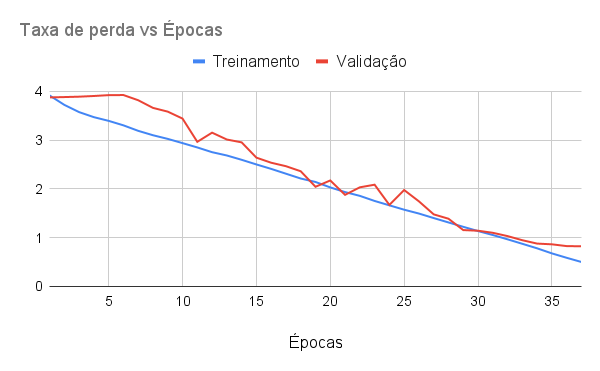
\includegraphics[width=.50\textwidth]{imagens/resultados_discussao/architecture/inception_v3/original/perda.png}\hfill
    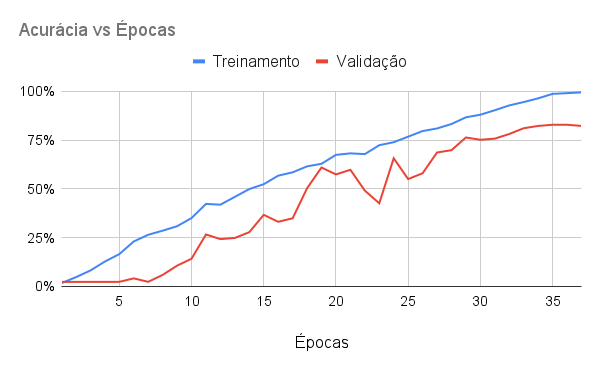
\includegraphics[width=.50\textwidth]{imagens/resultados_discussao/architecture/inception_v3/original/acuracia.png}\bigbreak    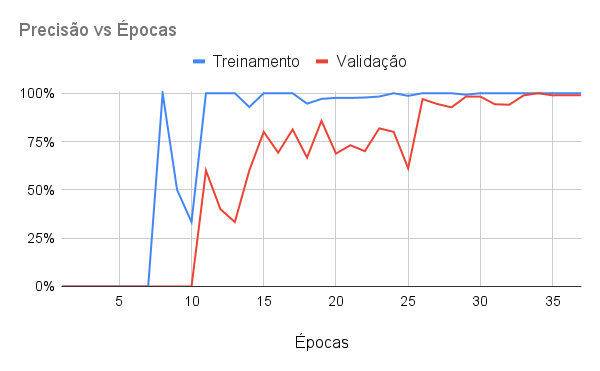
\includegraphics[width=.50\textwidth]{imagens/resultados_discussao/architecture/inception_v3/original/precisao.png}\hfill
    \includegraphics[width=.50\textwidth]{imagens/resultados_discussao/architecture/inception_v3/original/revocacao.png}
    \label{fig:inception_v3_dados_originais}
    \source{Danilo Assunção, 2022}
\end{figure}

Para este modelo, foram obtidos os resultados e coletadas as suas medidas, sendo elas apresentadas no Quadro \ref{quad:resultados_teste_inception_v3_com_dados_originais}.

\begin{quadro}[H]
\caption{Resultados do teste com a Inception v3 + Dados originais}
\label{quad:resultados_teste_inception_v3_com_dados_originais}
\centering
\begin{tabular}{|l|l|l|l|l|l|l|l|}
\cline{1-8}
Épocas & Perda & Acurácia & Precisão & Revocação & Medida F & Acertos & Erros \\ \hline
37 & 0,87 & 81,15\% & 100,00\% & 51,83\% & 68,28\% & 155 & 36 \\
\cline{1-8}
\end{tabular}
\source{Danilo Assunção, 2022}
\end{quadro}

No teste deste experimento foi alcançado um valor de 68,28\% para a Medida F, que é a medida sendo utilizada para comparativo neste trabalho, e, considerando que este modelo não possui nenhuma técnica de aumento de dados e transferência de aprendizado, ele conseguiu atingir um valor de 81,15\% de Acurácia, acertando um total de 155 imagens e errando 36 imagens.

No experimento seguinte, considerando a aplicação da técnica de aumento de dados através do uso do conjunto de dados aumentado, o modelo não mais demonstrou melhorias até seu treinamento por 13 épocas. Os dados adquiridos no treinamento deste modelo podem ser vistos na Figura \ref{fig:inception_v3_dados_aumentados}.

\begin{figure}[H]
    \centering
    \caption{Resultados do treinamento da Inception v3 + Dados aumentados}
    \includegraphics[width=.50\textwidth]{imagens/resultados_discussao/architecture/inception_v3/augmented/perda.png}\hfill
    \includegraphics[width=.50\textwidth]{imagens/resultados_discussao/architecture/inception_v3/augmented/acuracia.png}\bigbreak    \includegraphics[width=.50\textwidth]{imagens/resultados_discussao/architecture/inception_v3/augmented/precisao.png}\hfill
    \includegraphics[width=.50\textwidth]{imagens/resultados_discussao/architecture/inception_v3/augmented/revocacao.png}
    \label{fig:inception_v3_dados_aumentados}
    \source{Danilo Assunção, 2022}
\end{figure}

Para a fase de teste deste modelo utilizando os dados aumentados, temos a visualização dos resultados obtidos no Quadro \ref{quad:resultados_teste_inception_v3_com_dados_aumentados}.

\begin{quadro}[H]
\caption{Resultados do teste com a Inception v3 + Dados aumentados}
\label{quad:resultados_teste_inception_v3_com_dados_aumentados}
\centering
\begin{tabular}{|l|l|l|l|l|l|l|l|}
\cline{1-8}
Épocas & Perda & Acurácia & Precisão & Revocação & Medida F & Acertos & Erros \\ \hline
13 & 0,28 & 91,10\% & 91,44\% & 89,53\% & 90,48\% & 174 & 17 \\
\cline{1-8}
\end{tabular}
\source{Danilo Assunção, 2022}
\end{quadro}

Comparando a Medida F e a Acurácia resultante dos dois últimos testes, o modelo que utilizou o conjunto de dados aumentado teve um acréscimo de 22,20\% em sua Medida F e 9,95\% em sua Acurácia, somente ampliando a quantidade de imagens do conjunto de dados. É observável também que, além do desempenho ter sido melhorado com o aumento de dados, a quantidade de épocas necessárias para se ter este resultado foi menor em relação ao modelo que não usa o aumento de dados, tendo utilizado 24 épocas a menos para atingir resultados melhores neste modelo. Sendo assim, o uso da Inception v3 com aumento de dados, demonstrou ser superior em comparação ao experimento que utiliza o conjunto de dados original.

Considerando os modelos anteriores, foram também executados testes utilizando o conjunto de dados original e o conjunto de dados aumentado, em união com a técnica de transferência de aprendizado. O primeiro teste foi feito empregando o conjunto de dados original com a técnica de transferência de aprendizado. Seus dados obtidos no processo de treinamento podem ser observados na Figura \ref{fig:inception_v3_original_transferencia_aprendizado}.

\begin{figure}[H]
    \centering
    \caption{Resultados do treinamento com a Inception v3 + Dados originais + Transferência de aprendizado}
    \includegraphics[width=.50\textwidth]{imagens/resultados_discussao/architecture/inception_v3/transfer_learning/original/perda.png}\hfill
    \includegraphics[width=.50\textwidth]{imagens/resultados_discussao/architecture/inception_v3/transfer_learning/original/acuracia.png}\bigbreak    \includegraphics[width=.50\textwidth]{imagens/resultados_discussao/architecture/inception_v3/transfer_learning/original/precisao.png}\hfill
    \includegraphics[width=.50\textwidth]{imagens/resultados_discussao/architecture/inception_v3/transfer_learning/original/revocacao.png}
    \label{fig:inception_v3_original_transferencia_aprendizado}
    \source{Danilo Assunção, 2022}
\end{figure}

Para o teste deste modelo foi coletado os valores que podem ser vistos através do Quadro \ref{quad:test_inception_v3_original_transfer_learning}.

\begin{quadro}[H]
\caption{Resultados do teste com a Inception v3 + Dados originais + Transferência de aprendizado}
\label{quad:test_inception_v3_original_transfer_learning}
\centering
\begin{tabular}{|l|l|l|l|l|l|l|l|}
\cline{1-8}
Épocas & Perda & Acurácia & Precisão & Revocação & Medida F & Acertos & Erros \\ \hline
37 & 0,87 & 81,15\% & 100,00\% & 51,83\% & 68,28\% & 155 & 36 \\
\cline{1-8}
\end{tabular}
\source{Danilo Assunção, 2022}
\end{quadro}

Por fim, o último experimento utilizando esta arquitetura foi feito aplicando ambas as técnicas de aumento de dados e de transferência de aprendizado. Os resultados obtidos durante o treinamento deste modelo, usando ambas as técnicas, podem ser analisados através da Figura \ref{fig:inception_v3_augmented_transfer_learning}.

\begin{figure}[H]
    \centering
    \caption{Resultados do treinamento com a Inception v3 + Dados aumentados + Transferência de aprendizado}
    \includegraphics[width=.50\textwidth]{imagens/resultados_discussao/architecture/inception_v3/transfer_learning/augmented/perda.png}\hfill
    \includegraphics[width=.50\textwidth]{imagens/resultados_discussao/architecture/inception_v3/transfer_learning/augmented/acuracia.png}\bigbreak    \includegraphics[width=.50\textwidth]{imagens/resultados_discussao/architecture/inception_v3/transfer_learning/augmented/precisao.png}\hfill
    \includegraphics[width=.50\textwidth]{imagens/resultados_discussao/architecture/inception_v3/transfer_learning/augmented/revocacao.png}
    \label{fig:inception_v3_augmented_transfer_learning}
    \source{Danilo Assunção, 2022}
\end{figure}

Em relação ao modelo que usa transferência de aprendizado com os dados originais, este exemplo precisou de apenas 6 épocas, obtendo seu melhor resultado em 31 épocas a menos em comparação ao modelo anterior. Os dados do teste deste experimento podem ser visualizados no Quadro \ref{quad:test_inception_v3_augmented_transfer_learning}.

\begin{quadro}[H]
\caption{Resultados do teste com a Inception v3 + Dados aumentados + Transferência de aprendizado}
\label{quad:test_inception_v3_augmented_transfer_learning}
\centering
\begin{tabular}{|l|l|l|l|l|l|l|l|}
\cline{1-8}
Épocas & Perda & Acurácia & Precisão & Revocação & Medida F & Acertos & Erros \\ \hline
6 & 0,18 & 94,24\% & 95,19\% & 93,19\% & 94,18\% & 180 & 11 \\
\cline{1-8}
\end{tabular}
\source{Danilo Assunção, 2022}
\end{quadro}

Os resultados em termos de desempenho deste último modelo, demonstraram melhores valores em comparação com a Medida F e Acurácia do experimento que utiliza a técnica de transferência de aprendizado com o conjunto de dados original, tendo obtido uma melhoria de 25,90\% em sua Medida F e 13,09\% na Acurácia, utilizando 31 épocas a menos do que o modelo anterior. 

Por apresentarem os maiores resultados, foi feita uma comparação com este último experimento em relação ao experimento que utiliza apenas o conjunto de dados aumentado, em que, este último experimento obteve um desempenho melhor, atingindo um aumento de 3,70\% em sua Medida F e 3,14\% em sua Acurácia, treinando por 7 épocas a menos do que o modelo comparado.

\subsection{ResNet-152}
\label{subsec:result_resnet_152}
ResNet-152 é uma arquitetura de rede neural convolucional da família ResNet, possuindo uma profundidade de 152 camadas. A ResNet-152 é 8 vezes mais profunda do que as redes da família VGG, entretanto, dado a sua arquitetura, a ResNet-152 ainda possui menor complexidade \cite{he2016deep} devido a certas condições presentes nesta arquitetura. 

Para a arquitetura ResNet-152, o primeiro experimento realizado foi utilizando o conjunto de dados original. Este modelo foi treinado por 35 épocas até não haver mais melhorias em seus resultados. A seguir, é possível visualizar os resultados obtidos na fase de treinamento para este experimento, através da Figura \ref{fig:resnet_152_dados_originais}.

\begin{figure}[H]
    \centering
    \caption{Resultados do treinamento com a ResNet-152 + Dados originais}
    \includegraphics[width=.50\textwidth]{imagens/resultados_discussao/architecture/resnet_152/original/perda.png}\hfill
    \includegraphics[width=.50\textwidth]{imagens/resultados_discussao/architecture/resnet_152/original/acuracia.png}\bigbreak    \includegraphics[width=.50\textwidth]{imagens/resultados_discussao/architecture/resnet_152/original/precisao.png}\hfill
    \includegraphics[width=.50\textwidth]{imagens/resultados_discussao/architecture/resnet_152/original/revocacao.png}
    \label{fig:resnet_152_dados_originais}
    \source{Danilo Assunção, 2022}
\end{figure}

Para este modelo, foram obtidos os resultados e coletadas as suas medidas, sendo elas apresentadas no Quadro \ref{quad:resultados_teste_resnet_152_com_dados_originais}.

\begin{quadro}[H]
\caption{Resultados do teste com a ResNet-152 + Dados originais}
\label{quad:resultados_teste_resnet_152_com_dados_originais}
\centering
\begin{tabular}{|l|l|l|l|l|l|l|l|}
\cline{1-8}
Épocas & Perda & Acurácia & Precisão & Revocação & Medida F & Acertos & Erros \\ \hline
35 & 1,34 & 69,11\% & 90,32\% & 29,32\% & 44,27\% & 132 & 59 \\
\cline{1-8}
\end{tabular}
\source{Danilo Assunção, 2022}
\end{quadro}

No experimento seguinte, foi feita a aplicação da técnica de aumento de dados através do uso do conjunto de dados aumentado, em que o modelo foi treinado por 20 épocas até não demonstrar mais melhorias em seu desempenho. Os dados adquiridos no treinamento deste modelo podem ser vistos na Figura \ref{fig:resnet_152_dados_aumentados}.

\begin{figure}[H]
    \centering
    \caption{Resultados do treinamento da ResNet-152 + Dados aumentados}
    \includegraphics[width=.50\textwidth]{imagens/resultados_discussao/architecture/resnet_152/augmented/perda.png}\hfill
    \includegraphics[width=.50\textwidth]{imagens/resultados_discussao/architecture/resnet_152/augmented/acuracia.png}\bigbreak    \includegraphics[width=.50\textwidth]{imagens/resultados_discussao/architecture/resnet_152/augmented/precisao.png}\hfill
    \includegraphics[width=.50\textwidth]{imagens/resultados_discussao/architecture/resnet_152/augmented/revocacao.png}
    \label{fig:resnet_152_dados_aumentados}
    \source{Danilo Assunção, 2022}
\end{figure}

Para a fase de teste deste modelo utilizando os dados aumentados, temos a visualização dos resultados obtidos no Quadro \ref{quad:resultados_teste_resnet_152_com_dados_aumentados}.

\begin{quadro}[H]
\caption{Resultados do teste com a ResNet-152 + Dados aumentados}
\label{quad:resultados_teste_resnet_152_com_dados_aumentados}
\centering
\begin{tabular}{|l|l|l|l|l|l|l|l|}
\cline{1-8}
Épocas & Perda & Acurácia & Precisão & Revocação & Medida F & Acertos & Erros \\ \hline
20 & 0,22 & 93,19\% & 94,18\% & 93,19\% & 93,68\% & 178 & 13 \\
\cline{1-8}
\end{tabular}
\source{Danilo Assunção, 2022}
\end{quadro}

Comparando a Medida F e a Acurácia resultante dos dois últimos testes, o modelo que utilizou o conjunto de dados aumentado teve um acréscimo de 49,41\% em sua Medida F e 24,08\% em sua Acurácia, somente ampliando a quantidade de imagens do conjunto de dados. Contudo, além do desempenho ter sido melhorado com o aumento de dados, a quantidade de épocas necessárias para se ter este resultado foi menor em relação ao modelo que usa o conjunto de dados original, tendo utilizado 15 épocas a menos para se atingir estes resultados.

O teste a seguir foi feito empregando o conjunto de dados original com a técnica de transferência de aprendizado. Seus dados obtidos no processo de treinamento podem ser observados na Figura \ref{fig:resnet_152_original_transferencia_aprendizado}.

\begin{figure}[H]
    \centering
    \caption{Resultados do treinamento com a ResNet-152 + Dados originais + Transferência de aprendizado}
    \includegraphics[width=.50\textwidth]{imagens/resultados_discussao/architecture/resnet_152/transfer_learning/original/perda.png}\hfill
    \includegraphics[width=.50\textwidth]{imagens/resultados_discussao/architecture/resnet_152/transfer_learning/original/acuracia.png}\bigbreak    \includegraphics[width=.50\textwidth]{imagens/resultados_discussao/architecture/resnet_152/transfer_learning/original/precisao.png}\hfill
    \includegraphics[width=.50\textwidth]{imagens/resultados_discussao/architecture/resnet_152/transfer_learning/original/revocacao.png}
    \label{fig:resnet_152_original_transferencia_aprendizado}
    \source{Danilo Assunção, 2022}
\end{figure}

Para o teste deste modelo foi coletado os valores que podem ser vistos através do Quadro \ref{quad:test_resnet_152_original_transfer_learning}.

\begin{quadro}[H]
\caption{Resultados do teste com a ResNet-152 + Dados originais + Transferência de aprendizado}
\label{quad:test_resnet_152_original_transfer_learning}
\centering
\begin{tabular}{|l|l|l|l|l|l|l|l|}
\cline{1-8}
Épocas & Perda & Acurácia & Precisão & Revocação & Medida F & Acertos & Erros \\ \hline
37 & 0,40 & 93,72\% & 96,91\% & 82,20\% & 88,95\% & 179 & 12 \\
\cline{1-8}
\end{tabular}
\source{Danilo Assunção, 2022}
\end{quadro}

Por fim, o último experimento utilizando esta arquitetura foi feito aplicando ambas as técnicas de aumento de dados e de transferência de aprendizado. Os resultados obtidos durante o treinamento deste modelo, usando ambas as técnicas, podem ser analisados através da Figura \ref{fig:resnet_152_augmented_transfer_learning}.

\begin{figure}[H]
    \centering
    \caption{Resultados do treinamento com a ResNet-152 + Dados aumentados + Transferência de aprendizado}
    \includegraphics[width=.50\textwidth]{imagens/resultados_discussao/architecture/resnet_152/transfer_learning/augmented/perda.png}\hfill
    \includegraphics[width=.50\textwidth]{imagens/resultados_discussao/architecture/resnet_152/transfer_learning/augmented/acuracia.png}\bigbreak    \includegraphics[width=.50\textwidth]{imagens/resultados_discussao/architecture/resnet_152/transfer_learning/augmented/precisao.png}\hfill
    \includegraphics[width=.50\textwidth]{imagens/resultados_discussao/architecture/resnet_152/transfer_learning/augmented/revocacao.png}
    \label{fig:resnet_152_augmented_transfer_learning}
    \source{Danilo Assunção, 2022}
\end{figure}

Os dados do teste deste experimento podem ser visualizados no Quadro \ref{quad:test_resnet_152_augmented_transfer_learning}.

\begin{quadro}[H]
\caption{Resultados do teste com a ResNet-152 + Dados aumentados + Transferência de aprendizado}
\label{quad:test_resnet_152_augmented_transfer_learning}
\centering
\begin{tabular}{|l|l|l|l|l|l|l|l|}
\cline{1-8}
Épocas & Perda & Acurácia & Precisão & Revocação & Medida F & Acertos & Erros \\ \hline
6 & 0,10 & 96,34\% & 96,34\% & 96,34\% & 96,34\% & 184 & 7 \\
\cline{1-8}
\end{tabular}
\source{Danilo Assunção, 2022}
\end{quadro}

Os resultados em termos de desempenho deste último modelo, demonstraram melhores valores em comparação com a Medida F e Acurácia do experimento que utiliza a técnica de transferência de aprendizado com o conjunto de dados original, tendo obtido uma melhoria de 7,39\% em sua Medida F e 2,62\% na Acurácia, utilizando 31 épocas a menos do que o modelo anterior. 

Uma comparação foi realizada a partir dos dois experimentos que trouxeram os maiores resultados, sendo eles o último experimento e o experimento que utiliza apenas o conjunto de dados aumentado. O último experimento acabou por ter um desempenho melhor ao atingir um aumento de 2,66\% em sua Medida F e 3,15\% em sua Acurácia, apresentando esse resultado ao treinar por 14 épocas a menos do que o modelo comparado e utilizando ambas as técnicas.

\subsection{VGG16}
VGG é uma arquitetura de CNN clássica, baseada em uma análise de como aumentar a profundidade de tais redes, proposta em \citeonline{simonyan2014very}. A VGG16 é uma arquitetura que faz parte da família de arquiteturas VGG contendo um total de 16 camadas.

Para a arquitetura VGG16, o primeiro experimento realizado foi utilizando o conjunto de dados original. Este modelo foi treinado por 42 épocas até não haver mais melhorias em seus resultados. A seguir, é possível visualizar os resultados obtidos na fase de treinamento para este experimento, através da Figura \ref{fig:vgg_16_dados_originais}.

\begin{figure}[H]
    \centering
    \caption{Resultados do treinamento com a VGG16 + Dados originais}
    \includegraphics[width=.50\textwidth]{imagens/resultados_discussao/architecture/vgg_16/original/perda.png}\hfill
    \includegraphics[width=.50\textwidth]{imagens/resultados_discussao/architecture/vgg_16/original/acuracia.png}\bigbreak    \includegraphics[width=.50\textwidth]{imagens/resultados_discussao/architecture/vgg_16/original/precisao.png}\hfill
    \includegraphics[width=.50\textwidth]{imagens/resultados_discussao/architecture/vgg_16/original/revocacao.png}
    \label{fig:vgg_16_dados_originais}
    \source{Danilo Assunção, 2022}
\end{figure}

Para este modelo, foram obtidos os resultados e coletadas as suas medidas, sendo elas apresentadas no Quadro \ref{quad:resultados_teste_vgg_16_com_dados_originais}.

\begin{quadro}[H]
\caption{Resultados do teste com a VGG16 + Dados originais}
\label{quad:resultados_teste_vgg_16_com_dados_originais}
\centering
\begin{tabular}{|l|l|l|l|l|l|l|l|}
\cline{1-8}
Épocas & Perda & Acurácia & Precisão & Revocação & Medida F & Acertos & Erros \\ \hline
42 & 1,05 & 79,06\% & 81,87\% & 78,01\% & 79,89\% & 151 & 40 \\
\cline{1-8}
\end{tabular}
\source{Danilo Assunção, 2022}
\end{quadro}

No experimento seguinte, foi feita a aplicação da técnica de aumento de dados através do uso do conjunto de dados aumentado, com este modelo sendo treinado por um total de 25 épocas até não demonstrar mais melhorias em seu desempenho. Os dados adquiridos no treinamento deste modelo podem ser vistos na Figura \ref{fig:vgg_16_dados_aumentados}.

\begin{figure}[H]
    \centering
    \caption{Resultados do treinamento da VGG16 + Dados aumentados}
    \includegraphics[width=.50\textwidth]{imagens/resultados_discussao/architecture/vgg_16/augmented/perda.png}\hfill
    \includegraphics[width=.50\textwidth]{imagens/resultados_discussao/architecture/vgg_16/augmented/acuracia.png}\bigbreak    \includegraphics[width=.50\textwidth]{imagens/resultados_discussao/architecture/vgg_16/augmented/precisao.png}\hfill
    \includegraphics[width=.50\textwidth]{imagens/resultados_discussao/architecture/vgg_16/augmented/revocacao.png}
    \label{fig:vgg_16_dados_aumentados}
    \source{Danilo Assunção, 2022}
\end{figure}

Para a fase de teste deste modelo utilizando os dados aumentados, temos a visualização dos resultados obtidos no Quadro \ref{quad:resultados_teste_vgg_16_com_dados_aumentados}.

\begin{quadro}[H]
\caption{Resultados do teste com a VGG16 + Dados aumentados}
\label{quad:resultados_teste_vgg_16_com_dados_aumentados}
\centering
\begin{tabular}{|l|l|l|l|l|l|l|l|}
\cline{1-8}
Épocas & Perda & Acurácia & Precisão & Revocação & Medida F & Acertos & Erros \\ \hline
25 & 1,33 & 77,49\% & 79,35\% & 76,44\% & 77,87\% & 148 & 43 \\
\cline{1-8}
\end{tabular}
\source{Danilo Assunção, 2022}
\end{quadro}

Comparando a Medida F e a Acurácia resultante dos dois últimos testes, o modelo que utilizou o conjunto de dados original ainda teve um maior desempenho com relação ao experimento que usa conjunto de dados aumentado, tendo uma diferença de 2,02\% na Medida F e 1,57\% na Acurácia. Este foi o primeiro experimento no qual a técnica de aumento de dados não demonstrou melhores resultados com relação ao experimento usando apenas o conjunto de dados original. Entretanto, ainda houve uma diferença de 17 épocas para que o experimento que usa os dados originais obtivesse tais resultados.

O teste a seguir foi feito aplicando o conjunto de dados original com a técnica de transferência de aprendizado. Os dados obtidos no processo de treinamento deste experimento podem ser vistos na Figura \ref{fig:vgg_16_original_transferencia_aprendizado}.

\begin{figure}[H]
    \centering
    \caption{Resultados do treinamento com a VGG16 + Dados originais + Transferência de aprendizado}
    \includegraphics[width=.50\textwidth]{imagens/resultados_discussao/architecture/vgg_16/transfer_learning/original/perda.png}\hfill
    \includegraphics[width=.50\textwidth]{imagens/resultados_discussao/architecture/vgg_16/transfer_learning/original/acuracia.png}\bigbreak    \includegraphics[width=.50\textwidth]{imagens/resultados_discussao/architecture/vgg_16/transfer_learning/original/precisao.png}\hfill
    \includegraphics[width=.50\textwidth]{imagens/resultados_discussao/architecture/vgg_16/transfer_learning/original/revocacao.png}
    \label{fig:vgg_16_original_transferencia_aprendizado}
    \source{Danilo Assunção, 2022}
\end{figure}

Para o teste deste modelo foi coletado os valores que podem ser vistos através do Quadro \ref{quad:test_vgg_16_original_transfer_learning}.

\begin{quadro}[H]
\caption{Resultados do teste com a VGG16 + Dados originais + Transferência de aprendizado}
\label{quad:test_vgg_16_original_transfer_learning}
\centering
\begin{tabular}{|l|l|l|l|l|l|l|l|}
\cline{1-8}
Épocas & Perda & Acurácia & Precisão & Revocação & Medida F & Acertos & Erros \\ \hline
34 & 0,31 & 90,58\% & 90,58\% & 90,58\% & 90,58\% & 173 & 18 \\
\cline{1-8}
\end{tabular}
\source{Danilo Assunção, 2022}
\end{quadro}

E por último, foi feito o teste aplicando as técnicas de aumento de dados e de transferência de aprendizado. Os resultados obtidos durante o treinamento deste modelo, usando ambas as técnicas, podem ser analisados através da Figura \ref{fig:vgg_16_augmented_transfer_learning}.

\begin{figure}[H]
    \centering
    \caption{Resultados do treinamento com a VGG16 + Dados aumentados + Transferência de aprendizado}
    \includegraphics[width=.50\textwidth]{imagens/resultados_discussao/architecture/vgg_16/transfer_learning/augmented/perda.png}\hfill
    \includegraphics[width=.50\textwidth]{imagens/resultados_discussao/architecture/vgg_16/transfer_learning/augmented/acuracia.png}\bigbreak    \includegraphics[width=.50\textwidth]{imagens/resultados_discussao/architecture/vgg_16/transfer_learning/augmented/precisao.png}\hfill
    \includegraphics[width=.50\textwidth]{imagens/resultados_discussao/architecture/vgg_16/transfer_learning/augmented/revocacao.png}
    \label{fig:vgg_16_augmented_transfer_learning}
    \source{Danilo Assunção, 2022}
\end{figure}

Os dados do teste deste experimento podem ser visualizados no Quadro \ref{quad:test_vgg_16_augmented_transfer_learning}.

\begin{quadro}[H]
\caption{Resultados do teste com a VGG16 + Dados aumentados + Transferência de aprendizado}
\label{quad:test_vgg_16_augmented_transfer_learning}
\centering
\begin{tabular}{|l|l|l|l|l|l|l|l|}
\cline{1-8}
Épocas & Perda & Acurácia & Precisão & Revocação & Medida F & Acertos & Erros \\ \hline
8 & 0,26 & 93,19\% & 93,19\% & 93,19\% & 93,19\% & 178 & 13 \\
\cline{1-8}
\end{tabular}
\source{Danilo Assunção, 2022}
\end{quadro}

Os resultados em termos de desempenho deste último modelo, demonstraram melhores valores em comparação com a Medida F e Acurácia do experimento que utiliza a técnica de transferência de aprendizado com o conjunto de dados original, tendo obtido uma melhoria de 2,61\% em sua Medida F e 2,61\% na Acurácia e utilizando 26 épocas a menos do que o modelo anterior.

Neste experimento utilizando a arquitetura VGG16, os dois modelos que melhor desempenharam foram ambos os exemplares que utilizam a técnica de transferência de aprendizado, sendo assim, para esta arquitetura, a técnica de transferência de aprendizado foi a que melhor auxiliou em termos de desempenho.

\subsection{VGG19}
VGG19 é uma arquitetura de CNN que pertence à família VGG, possuindo um total de 19 camadas que compõem a sua estrutura.

Para a arquitetura VGG19, o primeiro experimento realizado foi utilizando o conjunto de dados original. Este modelo foi treinado por 48 épocas até não apresentar mais melhorias em seus resultados. A seguir, é possível visualizar os resultados obtidos na fase de treinamento para este experimento, através da Figura \ref{fig:vgg_19_dados_originais}.

\begin{figure}[H]
    \centering
    \caption{Resultados do treinamento com a VGG19 + Dados originais}
    \includegraphics[width=.50\textwidth]{imagens/resultados_discussao/architecture/vgg_19/original/perda.png}\hfill
    \includegraphics[width=.50\textwidth]{imagens/resultados_discussao/architecture/vgg_19/original/acuracia.png}\bigbreak    \includegraphics[width=.50\textwidth]{imagens/resultados_discussao/architecture/vgg_19/original/precisao.png}\hfill
    \includegraphics[width=.50\textwidth]{imagens/resultados_discussao/architecture/vgg_19/original/revocacao.png}
    \label{fig:vgg_19_dados_originais}
    \source{Danilo Assunção, 2022}
\end{figure}

Para este modelo, foram obtidos os resultados e coletadas as suas medidas, sendo elas apresentadas no Quadro \ref{quad:resultados_teste_vgg_19_com_dados_originais}.

\begin{quadro}[H]
\caption{Resultados do teste com a VGG19 + Dados originais}
\label{quad:resultados_teste_vgg_19_com_dados_originais}
\centering
\begin{tabular}{|l|l|l|l|l|l|l|l|}
\cline{1-8}
Épocas & Perda & Acurácia & Precisão & Revocação & Medida F & Acertos & Erros \\ \hline
48 & 0,84 & 82,72\% & 84,41\% & 82,20\% & 83,29\% & 158 & 33 \\
\cline{1-8}
\end{tabular}
\source{Danilo Assunção, 2022}
\end{quadro}

No experimento seguinte, foi feita a aplicação da técnica de aumento de dados através do uso do conjunto de dados aumentado, em que o modelo foi treinado por um total de 18 épocas até não demonstrar mais melhorias em seu desempenho. Os dados adquiridos no treinamento deste modelo podem ser vistos na Figura \ref{fig:vgg_19_dados_aumentados}.

\begin{figure}[H]
    \centering
    \caption{Resultados do treinamento da VGG19 + Dados aumentados}
    \includegraphics[width=.50\textwidth]{imagens/resultados_discussao/architecture/vgg_19/augmented/perda.png}\hfill
    \includegraphics[width=.50\textwidth]{imagens/resultados_discussao/architecture/vgg_19/augmented/acuracia.png}\bigbreak    \includegraphics[width=.50\textwidth]{imagens/resultados_discussao/architecture/vgg_19/augmented/precisao.png}\hfill
    \includegraphics[width=.50\textwidth]{imagens/resultados_discussao/architecture/vgg_19/augmented/revocacao.png}
    \label{fig:vgg_19_dados_aumentados}
    \source{Danilo Assunção, 2022}
\end{figure}

Para a fase de teste deste modelo utilizando os dados aumentados, temos a visualização dos resultados obtidos no Quadro \ref{quad:resultados_teste_vgg_19_com_dados_aumentados}.

\begin{quadro}[H]
\caption{Resultados do teste com a VGG19 + Dados aumentados}
\label{quad:resultados_teste_vgg_19_com_dados_aumentados}
\centering
\begin{tabular}{|l|l|l|l|l|l|l|l|}
\cline{1-8}
Épocas & Perda & Acurácia & Precisão & Revocação & Medida F & Acertos & Erros \\ \hline
18 & 1,47 & 80,10\% & 79,89\% & 79,06\% & 79,47\% & 153 & 38 \\
\cline{1-8}
\end{tabular}
\source{Danilo Assunção, 2022}
\end{quadro}

Comparando a Medida F e a Acurácia resultante dos dois últimos testes, o modelo que utilizou o conjunto de dados original ainda teve um maior desempenho em relação ao experimento que usa conjunto de dados aumentado, tendo uma diferença de 3,82\% na Medida F e 2,62\% na Acurácia, tendo percorrido 30 épocas a mais para se atingir estes resultados. Este foi um resultado similar ao cenário visto na VGG16, onde o modelo que usa o conjunto de dados aumentado obteve um desempenho menor em relação ao modelo que usa o conjunto de dados original.

O teste a seguir foi feito aplicando o conjunto de dados original com a técnica de transferência de aprendizado. Os dados obtidos no processo de treinamento deste experimento podem ser vistos na Figura \ref{fig:vgg_19_original_transferencia_aprendizado}.

\begin{figure}[H]
    \centering
    \caption{Resultados do treinamento com a VGG19 + Dados originais + Transferência de aprendizado}
    \includegraphics[width=.50\textwidth]{imagens/resultados_discussao/architecture/vgg_19/transfer_learning/original/perda.png}\hfill
    \includegraphics[width=.50\textwidth]{imagens/resultados_discussao/architecture/vgg_19/transfer_learning/original/acuracia.png}\bigbreak    \includegraphics[width=.50\textwidth]{imagens/resultados_discussao/architecture/vgg_19/transfer_learning/original/precisao.png}\hfill
    \includegraphics[width=.50\textwidth]{imagens/resultados_discussao/architecture/vgg_19/transfer_learning/original/revocacao.png}
    \label{fig:vgg_19_original_transferencia_aprendizado}
    \source{Danilo Assunção, 2022}
\end{figure}

Para o teste deste modelo foi coletado os valores que podem ser vistos através do Quadro \ref{quad:test_vgg_19_original_transfer_learning}.

\begin{quadro}[H]
\caption{Resultados do teste com a VGG19 + Dados originais + Transferência de aprendizado}
\label{quad:test_vgg_19_original_transfer_learning}
\centering
\begin{tabular}{|l|l|l|l|l|l|l|l|}
\cline{1-8}
Épocas & Perda & Acurácia & Precisão & Revocação & Medida F & Acertos & Erros \\ \hline
23 & 0,51 & 89,01\% & 90,32\% & 87,96\% & 89,12\% & 170 & 21 \\
\cline{1-8}
\end{tabular}
\source{Danilo Assunção, 2022}
\end{quadro}

Por fim, foi executado o teste aplicando ambas as técnicas de aumento de dados e transferência de aprendizado. Os resultados obtidos durante o treinamento deste modelo podem ser analisados através da Figura \ref{fig:vgg_19_augmented_transfer_learning}.

\begin{figure}[H]
    \centering
    \caption{Resultados do treinamento com a VGG19 + Dados aumentados + Transferência de aprendizado}
    \includegraphics[width=.50\textwidth]{imagens/resultados_discussao/architecture/vgg_19/transfer_learning/augmented/perda.png}\hfill
    \includegraphics[width=.50\textwidth]{imagens/resultados_discussao/architecture/vgg_19/transfer_learning/augmented/acuracia.png}\bigbreak    \includegraphics[width=.50\textwidth]{imagens/resultados_discussao/architecture/vgg_19/transfer_learning/augmented/precisao.png}\hfill
    \includegraphics[width=.50\textwidth]{imagens/resultados_discussao/architecture/vgg_19/transfer_learning/augmented/revocacao.png}
    \label{fig:vgg_19_augmented_transfer_learning}
    \source{Danilo Assunção, 2022}
\end{figure}

Os dados do teste deste experimento podem ser visualizados no Quadro \ref{quad:test_vgg_19_augmented_transfer_learning}.

\begin{quadro}[H]
\caption{Resultados do teste com a VGG19 + Dados aumentados + Transferência de aprendizado}
\label{quad:test_vgg_19_augmented_transfer_learning}
\centering
\begin{tabular}{|l|l|l|l|l|l|l|l|}
\cline{1-8}
Épocas & Perda & Acurácia & Precisão & Revocação & Medida F & Acertos & Erros \\ \hline
5 & 0,27 & 94,24\% & 94,74\% & 94,24\% & 94,49\% & 180 & 11 \\
\cline{1-8}
\end{tabular}
\source{Danilo Assunção, 2022}
\end{quadro}

Os resultados em termos de desempenho deste último modelo, demonstraram melhores valores em comparação com a Medida F e Acurácia do experimento que utiliza a técnica de transferência de aprendizado com o conjunto de dados original, tendo obtido uma diferença superior de 5,37\% em sua Medida F e 5,23\% em na Acurácia utilizando 18 épocas a menos do que o modelo anterior.

Neste experimento utilizando a arquitetura VGG19, os dois modelos que melhor desempenharam foram também os exemplares que utilizam a técnica de transferência de aprendizado, sendo assim, para esta arquitetura, a técnica de transferência de aprendizado foi a que também melhor auxiliou em termos de desempenho para os modelos que usaram a arquitetura VGG.

\subsection{Conclusão}
Todas as arquiteturas de CNN utilizadas nos experimentos desta seção possuem suas especificidades, isto é, cada uma contém características que permitem a resolução de um determinado problema. Se tratando das técnicas de aumento de dados e transferência de aprendizado, a técnica que mais influenciou em termos de desempenho foi a técnica de aumento de dados, que proporcionou resultados relevantes para os modelos em comparação aos modelos que utilizaram o conjunto de dados original, entretanto, a técnica de transferência de aprendizado também teve uma participação no aspecto da quantidade de épocas nas quais esses modelos foram treinados, dado que, com o uso desta técnica, foi notado uma considerável queda na quantidade de épocas necessárias para se atingir certos resultados, e, com a união de ambas as técnicas, têm-se normalmente os mesmos comportamentos presentes ao mesmo tempo, elevando consideravelmente o resultado obtido nos testes, já que as medidas resultantes do modelo eram melhoradas e o número de épocas necessário para se atingir estes resultados eram menores. 

Um outro aspecto também observado através dos gráficos contendo as medidas obtidas na fase de treinamento dos experimentos, é a incidência de cenários com sobreajuste (Figura \ref{fig:inception_v3_original_transferencia_aprendizado}) ou subajuste, (Figura \ref{fig:resnet_152_dados_originais}) sendo tais cenários predominantemente encontrados apenas em modelos que utilizaram o conjunto de dados original, e dado este comportamento, foi possível identificar que as técnicas de aumento de dados e transparência ajudaram muito a mitigar casos de sobreajuste ou subajuste nos modelos que utilizam estes métodos, em principal a técnica de aumento de dados, tornando-se um bom indicativo que, para a prevenção de sobreajuste ou subajuste, o uso de técnicas de aumento de dados e transferência de aprendizado podem favorecer contra este tipo de problema, evitando que cenários deste tipo ocorram.

Concluindo, neste experimento o modelo que melhor desempenhou em termos de Acurácia e Medida F foi a arquitetura ResNet-152, que fez uso das técnicas de aumento de dados e transferência de aprendizado, e retornou o melhor resultado em relação aos outros modelos ao obter uma Acurácia e Medida F de 96,33\% respectivamente.

\section{Seleção do algoritmo de otimização}
Nesta seção serão abordados algumas experimentações com base na arquitetura de CNN extraída no primeiro experimento, isto é, utilizando-se da arquitetura de CNN selecionada na primeira experimentação (ResNet-152) e realizados outros testes em cima desta arquitetura, aplicando algoritmos de otimização distintos para verificar qual o algoritmo que possui o melhor resultado, em referência ao modelo proposto. O conjunto de dados considerado neste segundo experimento foi o conjunto de dados ampliado pela técnica de aumento de dados, visto que, a arquitetura selecionada no primeiro experimento obteve o melhor resultado utilizando o conjunto de dados aumentado. Contudo, para esta experimentação, foi feito o uso de alguns algoritmos de otimização para CNNs disponibilizados pela biblioteca utilizada nesta ferramenta, sendo estes algoritmos, SGD, Adagrad, Adadelta e Adamax. O detalhamento dos resultados obtidos do SGD já foram esclarecidos na Subseção \ref{subsec:result_resnet_152} a partir da Figura \ref{fig:resnet_152_augmented_transfer_learning}, sendo que no primeiro experimento, as CNNs utilizam por padrão o algoritmo de otimização SGD, e o resultado obtido neste experimento para as medidas, tanto a Acurácia quanto a Medida F, foi de 96,33\%. Para todos estes algoritmos, nenhum hiperparâmetro é alterado, além da estratégia que determina a taxa de aprendizado, definida na Seção \ref{sec:avaliacao}, ou seja, desconsiderando a taxa de aprendizado, o restante dos hiperparâmetros são os já definidos pela biblioteca utilizada pela ferramenta.

\subsection{Adagrad}
Adagrad é um algoritmo de otimização definido em \citeonline{duchi2011adaptive}, que aplica taxas de aprendizado específicas para os parâmetros da rede, que são adaptadas em relação à frequência com que um parâmetro é atualizado durante o treinamento. Quanto mais atualizações um parâmetro recebe, menores são as atualizações.

O primeiro passo deste teste foi feito executando o modelo selecionado no primeiro experimento que definia a arquitetura de CNN junto com o otimizador Adagrad. O treinamento deste modelo foi parado a partir da época 7, dado que não houve melhorias após esta época considerando os critérios de parada estabelecidos para o treinamento dos modelos em todos os experimentos. Os dados obtidos no treinamento deste modelo são mostrados através da Figura \ref{fig:adagrad_training}.

\begin{figure}[H]
    \centering
    \caption{Resultados do treinamento usando Adagrad}
    \includegraphics[width=.50\textwidth]{imagens/resultados_discussao/optimizer/adagrad/perda.png}\hfill
    \includegraphics[width=.50\textwidth]{imagens/resultados_discussao/optimizer/adagrad/acuracia.png}\bigbreak    \includegraphics[width=.50\textwidth]{imagens/resultados_discussao/optimizer/adagrad/precisao.png}\hfill
    \includegraphics[width=.50\textwidth]{imagens/resultados_discussao/optimizer/adagrad/revocacao.png}
    \label{fig:adagrad_training}
    \source{Danilo Assunção, 2022}
\end{figure}

Abaixo é exibido a partir do Quadro \ref{quad:test_adagrad} os dados obtidos no teste deste modelo depois da fase de treinamento.

\begin{quadro}[H]
\caption{Resultados do teste usando Adagrad}
\label{quad:test_adagrad}
\centering
\begin{tabular}{|l|l|l|l|l|l|l|l|}
\cline{1-8}
Épocas & Perda & Acurácia & Precisão & Revocação & Medida F & Acertos & Erros \\ \hline
7 & 0,13 & 94,76\% & 95,74\% & 94,24\% & 94,99\% & 181 & 10 \\
\cline{1-8}
\end{tabular}
\source{Danilo Assunção, 2022}
\end{quadro}

Considerando os resultados obtidos, foram de fato relevantes, porém se comparado com o modelo utilizando SGD, o Adagrad não desempenhou tão bem e isso pode ter ligação com a taxa de aprendizado utilizada na inicialização do algoritmo, dado que o valor foi estabelecido seguindo os valores já definidos para a avaliação deste trabalho. Comparando este modelo que usou Adagrad com o modelo que utilizou o otimizador SGD, é apresentado no teste, usando o Adagrad, uma queda na Medida F e Acurácia de 1,34\% e 1,57\% , respectivamente com 1 época a mais executada.

\subsection{Adadelta}
Com base na definição em \citeonline{zeiler2012adadelta}, Adadelta é um método de descida de gradiente (otimizador), que se baseia na taxa de aprendizagem adaptativa por dimensão para resolver duas desvantagens contidas em otimizadores como o Adagrad, sendo elas, o decaimento contínuo das taxas de aprendizado ao longo do treinamento que se torna infinitesimalmente pequena em algum ponto, dado que a partir de um certo número de iterações o modelo pode perder a capacidade de aprender novos padrões, e, respectivamente, a necessidade da definição manual de uma taxa de aprendizado global.

O primeiro passo deste teste foi feito executando o modelo selecionado no primeiro experimento que definia a arquitetura de CNN junto com o otimizador Adadelta. O treinamento deste modelo foi parado a partir da época 37, dado que não houve melhorias após esta época considerando os critérios de parada estabelecidos para o treinamento dos modelos em todos os experimentos. Os dados obtidos no treinamento deste modelo são mostrados através da Figura \ref{fig:adagrad_training}.

Na imagem \ref{fig:adadelta_training} 
\begin{figure}[H]
    \centering
    \caption{Resultados do treinamento usando Adadelta}
    \includegraphics[width=.50\textwidth]{imagens/resultados_discussao/optimizer/adadelta/perda.png}\hfill
    \includegraphics[width=.50\textwidth]{imagens/resultados_discussao/optimizer/adadelta/acuracia.png}\bigbreak    \includegraphics[width=.50\textwidth]{imagens/resultados_discussao/optimizer/adadelta/precisao.png}\hfill
    \includegraphics[width=.50\textwidth]{imagens/resultados_discussao/optimizer/adadelta/revocacao.png}
    \label{fig:adadelta_training}
    \source{Danilo Assunção, 2022}
\end{figure}

Abaixo é exibido, a partir do Quadro \ref{quad:test_adadelta}, os dados obtidos no teste deste modelo depois da fase de treinamento.

\begin{quadro}[H]
\caption{Resultados do teste usando Adadelta}
\label{quad:test_adadelta}
\centering
\begin{tabular}{|l|l|l|l|l|l|l|l|}
\cline{1-8}
Épocas & Perda & Acurácia & Precisão & Revocação & Medida F & Acertos & Erros \\ \hline
37 & 0,14 & 94,24\% & 95,65\% & 92,15\% & 93,87\% & 180 & 11 \\
\cline{1-8}
\end{tabular}
\source{Danilo Assunção, 2022}
\end{quadro}

Considerando os resultados obtidos, foram de fato relevantes, porém se comparado com o modelo utilizando SGD, o Adadelta teve um desempenho levemente inferior, isto é, comparando ambos os testes destes modelos, o que usou o Adadelta teve uma diferença abaixo do teste usando SGD de 2,46\% e 2,09\% na Medida F e Acurácia, respectivamente com 31 épocas a mais em ciclos de treinamento.

\subsection{Adamax}
Adamax é um algoritmo de otimização adaptativo sendo uma variante do algoritmo Adam, baseado na norma do infinito. Ambos foram detalhados em \citeonline{kingma2014adam}.

O primeiro passo deste teste foi realizado executando o modelo selecionado no primeiro experimento que definia a arquitetura de CNN junto com o otimizador Adamax. O treinamento deste modelo foi parado a partir da época 20, dado que não houve melhorias após esta época considerando os critérios de parada estabelecidos para o treinamento dos modelos em todos os experimentos. Os dados obtidos no treinamento deste modelo são mostrados através da Figura \ref{fig:adamax_training}.

\begin{figure}[H]
    \centering
    \caption{Resultados do treinamento usando Adamax}
    \includegraphics[width=.50\textwidth]{imagens/resultados_discussao/optimizer/adamax/perda.png}\hfill
    \includegraphics[width=.50\textwidth]{imagens/resultados_discussao/optimizer/adamax/acuracia.png}\bigbreak    \includegraphics[width=.50\textwidth]{imagens/resultados_discussao/optimizer/adamax/precisao.png}\hfill
    \includegraphics[width=.50\textwidth]{imagens/resultados_discussao/optimizer/adamax/revocacao.png}
    \label{fig:adamax_training}
    \source{Danilo Assunção, 2022}
\end{figure}

Abaixo é exibido, a partir do Quadro \ref{quad:test_adamax}, os dados obtidos no teste deste modelo depois da fase de treinamento.

\begin{quadro}[H]
\caption{Resultados do teste usando Adamax}
\label{quad:test_adamax}
\centering
\begin{tabular}{|l|l|l|l|l|l|l|l|}
\cline{1-8}
Épocas & Perda & Acurácia & Precisão & Revocação & Medida F & Acertos & Erros \\ \hline
12 & 0,08 & 97,91\% & 97,91\% & 97,91\% & 97,91\% & 187 & 4 \\
\cline{1-8}
\end{tabular}
\source{Danilo Assunção, 2022}
\end{quadro}

Considerando os resultados obtidos, foram de fato relevantes, porém se comparado com o modelo utilizando SGD, o Adamax obteve uma Medida F e Acurácia maior, atingindo uma baixa diferença de 1,58\% em ambas as medidas, porém com 6 épocas de treinamento a mais se comparado com o modelo que usou SGD.

\subsection{Conclusão}
Neste segundo experimento foi feito testes utilizando alguns algoritmos de otimização junto com a ResNet-152 (arquitetura selecionada no primeiro experimento), visando avaliar quais destes métodos fornecem o melhor resultado com base no problema que envolve a identificação das espécies de abelhas.

No escopo analisado, os algoritmos Adadelta e Adagrad demonstraram o menor desempenho em relação a todos os algoritmos avaliados. Neste último experimento, dois algoritmos obtiveram valores acima de 96\% de Acurácia e Medida F, sendo tais algoritmos, SGD e Adamax. O algoritmo Adamax foi o que atingiu a maior Acurácia e Medida F em comparação ao SGD, com uma diferença de 1,58\% para ambas as medidas citadas, ainda assim, isto foi obtido com um custo de 6 ciclos de treinamento adicionais, dado que o SGD foi o que convergiu mais rapidamente. Contudo, foi perceptível a vantagem no uso do Adamax que possui a capacidade de determinar a taxa de aprendizado de maneira automática com base no cenário abordado e este aspecto acaba por ser uma vantagem com relação à algoritmos como o SGD, dado que este tipo de algoritmo exige o ajuste manual de seus hiperparâmetros, como a taxa de aprendizado, o que torna mais complexo determinar o valor ideal neste contexto \cite{le2011optimization}. A partir disto, foi determinado que o algoritmo selecionado neste experimento é o Adamax, que alcançou uma Acurácia e Medida F de 97,91\%.

\section{Modelo final}
Para determinar o modelo final, foram conduzidos dois experimentos essenciais: a seleção da arquitetura de uma CNN e a seleção do algoritmo de otimização para a arquitetura selecionada e, com isso, foi possível determinar os componentes para a construção de um modelo em relação ao domínio abordado. No primeiro experimento, a arquitetura selecionada foi a ResNet-152 em conjunto com a técnica de transferência de aprendizado proposta neste trabalho, e esta arquitetura possibilitou o modelo a obter um resultado de 96,33\% nas medidas comparativas de Acurácia e Medida F. E para o segundo experimento, o que melhor desempenhou em termos de Acurácia e Medida F, junto à ResNet-152, foi o algoritmo Adamax que obteve respectivamente para ambas as medidas com um total de 97,91\%. Portanto, para o modelo final, foi definido utilizando a ResNet-152 com o algoritmo Adamax aplicando a técnica de aprendizado por transferência em cima do conjunto de dados ampliado, através da técnica de aumento de dados.

\section{Conclusão dos resultados}
Este capítulo detalhou todos os cenários analisados que levaram à escolha final do modelo com melhor desempenho. Com base nos valores anteriormente apresentados foi possível observar que, o uso de uma CNN com a utilização do conjunto de dados original, sem empregar nenhuma técnica específica para aprimoramento dos resultados, não seria possível alcançar valores relevantes devido ao seu baixo volume de dados, porém a utilização de técnicas de aumento de dados e transferência de aprendizado possibilitaram o uso de uma CNN para o domínio abordado. Para uma melhor visualização desta percepção, a seguir são apresentados alguns gráficos através das Figuras \ref{fig:medida_acuracia_medida_f_vs_grupo} e \ref{fig:media_epocas_vs_grupo}, que apresentam a média aritmética dos valores obtidos nas análises feitas através do primeiro experimento para determinados grupos de experimentação, sendo tais grupos, o conjunto de dados original (Original), o conjunto de dados aumentado (Aumentado), o conjunto de dados original com transferência de aprendizado (Original + Transferência) e o conjunto de dados aumentado com transferência de aprendizado (Aumentado + Transferência).

\begin{figure}[H]
    \centering
    \caption{Média aritmética de acurácia e medida F por Grupo}
    \includegraphics[width=1.0\textwidth]{imagens/resultados_discussao/conclusao/media_acuracia_e_medida_f_vs_grupo.png}
    \label{fig:medida_acuracia_medida_f_vs_grupo}
    \source{Danilo Assunção, 2022}
\end{figure}

Na Figura \ref{fig:medida_acuracia_medida_f_vs_grupo} temos a visualização das médias aritméticas de Acurácia e Medida F de cada grupo de experimentação, permitindo visualizar a influência das técnicas de aumento de dados e transferência de aprendizado nos experimentos em geral. O uso do conjunto de dados original, sem a aplicação de quaisquer técnicas, obteve em média 81,15\% na Acurácia e 79,89\% na Medida F, respectivamente, o mesmo conjunto de dados com o uso da transferência de aprendizado, resultaram na subida, em média, de 9,43\% na Acurácia e 9,06\% na Medida F. Neste caso, a transferência de aprendizado indicou aprimorar os resultados, em média, um pouco acima de 9\% para ambas as medidas e, dado o aumento da Medida F, indicando que este método também melhorou a precisão e revocação dos modelos testados. Para o grupo que usou o conjunto de dados aumentado, foi obtido nos testes em média uma Acurácia e Medida F de 91,10\% e 90,48\%, respectivamente, neste mesmo conjunto de dados com a união da técnica de transferência de aprendizado, as duas medidas subiram para 94,24\% e 94,18\%, ocorrendo um aumento em média de 4\% na Acurácia e Medida F. Analisando o grupo inicial, sem nenhum uso das técnicas propostas com o último grupo que utilizou ambas as técnicas de aumento de dados e transferência de aprendizado, é alcançado, em média, uma diferença de 13,09\% na Acurácia e 14,29\% na Medida F, o que enfatiza uma notável melhora quando tais técnicas são empregadas em um contexto com um conjunto de dados pequeno.

Não somente as medidas usadas para avaliar o modelo foram melhoradas, mas também a quantidade média de épocas necessárias para se obter tais resultados, conforme é apresentado pela Figura \ref{fig:media_epocas_vs_grupo}.

\begin{figure}[H]
    \centering
    \caption{Média de Épocas por Grupo}
    \includegraphics[width=1.0\textwidth]{imagens/resultados_discussao/conclusao/media_epocas_vs_grupo.png}
    \label{fig:media_epocas_vs_grupo}
    \source{Danilo Assunção, 2022}
\end{figure}

Neste gráfico que relaciona a quantidade média de épocas usadas no treinamento com relação aos grupos de experimentação deste trabalho, é possível observar que as técnicas de aumento de dados e transferência de aprendizado tiveram um impacto direto na diminuição da quantidade de épocas médias necessárias para se atingir os melhores resultados dos modelos, limitado ao valor de até 50 épocas. Considerando o grupo com o uso médio de épocas maior e menor, obteve-se uma diferença de 31 épocas (-83,78\%), demonstrando que as técnicas de aumento de dados e transferência de aprendizado, em conjunto, não somente melhoraram os resultados do modelo como também precisaram de menos épocas para obter estes resultados.

Concluindo, foi observado a partir dos experimentos que a aplicação de uma CNN pode ser uma ferramenta bem poderosa para o problema que envolve o reconhecimento das espécies de abelhas, contudo, dado o cenário com um baixo volume de dados, uma CNN pode não exibir bons resultados e, para solucionar este contexto, foi feito o uso de técnicas de aumento de dados e transferência de aprendizado, que auxiliam no aumento do desempenho do resultado do modelo proposto e permitindo que o modelo final selecionado obtivesse uma Acurácia e Medida F de 97,91\% nos testes executados.

%------------------------------------------------------------------------
% CAPITULO - Conclusão
%------------------------------------------------------------------------
\chapter{Conclusão}
O problema inicial que aborda a classificação das espécies de abelhas através da imagem de suas asas surgiu baseado em necessidades reais. Atualmente o responsável por realizar a classificação dessas espécies é um especialista que necessita de um vasto conhecimento para conseguir realizar essa tarefa que é totalmente manual, então dois problemas podem ser percebidos com isto, o primeiro é a necessidade de um especialista no assunto, o qual pode haver certa dificuldade de se encontrar e o segundo é o trabalho manual que é suscetível a erros. Diante disto, foi visto que através da imagem das asas de abelhas podem ser desenvolvidos métodos estatísticos que permitem realizar a classificação destas espécies, tais métodos podem ser realizados através de aprendizado de máquina que permitem automatizar a tarefa de identificação das espécies de maneira computadorizada. 

Com base nesta premissa, em \citeonline{rebelo2021fully} foi desenvolvido um importante trabalho que relaciona métodos que envolvem o pré-processamento e segmentação das imagens para extração de características relevantes contidas nestes componentes e a classificação automática destas espécies utilizando um algoritmo de aprendizado de máquina tradicional. Tal prática resultou em cenários promissores que demonstram resultados bem relevantes. Contudo, ainda mirando na evolução destes métodos, foi pensado no uso de algoritmos mais sofisticados incluídos no campo de aprendizado profundo para a classificação das espécies de abelhas, neste caso, algoritmos que permitam tal ação sem mais a necessidade do uso de métodos \textit{handcrafted} no processo que extrai as características das imagens, e o método escolhido para essa evolução foi viabilizar o uso de uma CNN para esta tarefa e neste trabalho é visto a experimentação da CNN para o domínio proposto que envolve a identificação das espécies de abelhas através de imagens de suas asas. 

Todavia, foi identificado que o uso de uma CNN envolve algumas premissas como uma quantidade grande de dados para se obter bons resultados e também há certa complexidade em sua execução. Para minimizar tais complexidades foi estudado neste trabalho certas técnicas encontradas na literatura que permitem driblar cenários que estão relacionados com o problema que é a baixa quantidade de dados disponíveis para se executar o treinamento adequado do modelo usando uma CNN e essas técnicas denominadas como técnica de aumento de dados e técnica de transferência de aprendizado foram utilizadas nos experimentos realizados e possibilitaram o uso de um método mais avançado em termos de extração de características e classificação atingindo resultados satisfatórios (97,91\% de Acurácia e Medida F) relacionados com o da \textit{baseline} definido neste trabalho.

\section{Limitações}
Em maioria, quase todos os hiperparâmetros considerados neste trabalho foram usados de maneira padrão fornecidos pela biblioteca utilizada na ferramenta proposta, ou seja, ainda existe um espaço para melhorias dos parâmetros de otimização. E outra limitação neste trabalho tem relação com a quantidade de imagens disponibilizadas para testes, devido ao conjunto de dados disponibilizado originalmente ter uma quantidade pequena de imagens disponíveis.

\section{Trabalhos futuros}
Abaixo são apresentadas algumas possibilidades que podem ser futuramente aplicadas como evolução deste projeto.

\begin{itemize}
  \item \textbf{Estudo de métodos que auxiliem na identificação de espécies de abelhas sem ferrão}: como citado na introdução, a identificação automática pode ser um desafio, principalmente para as abelhas sem ferrão que possuem características muito parecidas entre as espécies de mesmo grupo \cite{francoy2010morfometria} e isso de fato se mostrou válido dado que neste trabalho os resultados menos precisos foram relacionados ao grupo de espécie de abelhas sem ferrão denominado Austroplebeia. É viável que seja feito um estudo para encontrar algum método que permita que uma CNN consiga classificar espécies dentro destes grupos de espécies com maior precisão;
  
  \item \textbf{GAN para o aumento do conjunto de dados}: em \citeonline{shorten2019survey} é proposto um método sofisticado utilizando GANs (Redes adversárias generativas). A partir deste método, pode haver a criação de um método que irá permitir ter uma rede especializada na geração de imagens de asas de abelhas que ajudarão no crescimento do conjunto de dados;
  
  \item \textbf{Hiperparâmetros do otimizador da CNN}: utilização de métodos que permitam identificar os melhores hiperparâmetros para o algoritmo de otimização da CNN visando aumentar o seu desempenho e com isto aumentar consequentemente o desempenho da rede;
  
  \item \textbf{Teste de outros métodos de transferência de aprendizado}: em \citeonline{li2017learning} são definidas algumas técnicas além do método de extração de características e ajuste fino que podem também demonstrar bons resultados se aplicado neste domínio de identificação de espécies;
  
  \item \textbf{Arquitetura automática da CNN}: dada a complexidade contida em arquiteturas de CNN, alguns trabalhos estão realizando estudos que visam determinar a um domínio de maneira totalmente automática e não mais utilizando estruturas de CNN já pré-estabelecidas como as aplicadas neste trabalho. Um cenário é uso de algoritmos genéticos para a criação de arquiteturas de CNN de maneira automática como apresentado no trabalho de \citeonline{ahmed2019novel}.
\end{itemize}

% ----------------------------------------------------------
% ELEMENTOS PÓS-TEXTUAIS
% ----------------------------------------------------------
\postextual
% ----------------------------------------------------------

% ----------------------------------------------------------
% Referências bibliográficas
% ----------------------------------------------------------
\bibliography{referencias}

% ----------------------------------------------------------
% Glossário
% ----------------------------------------------------------
%
% Consulte o manual da classe abntex2 para orientações sobre o glossário.
%
%\glossary

% ----------------------------------------------------------
% Apêndices
% ----------------------------------------------------------

% ---
% Inicia os apêndices
% ---
\begin{apendicesenv}

% Imprime uma página indicando o início dos apêndices
%\partapendices

\chapter{Matriz confusão do modelo final}

\begin{figure}[ht]
    \centering
    \includegraphics[width=1.1\textwidth, angle=270]{imagens/apendice/confusion_matrix.png}
\end{figure}

\chapter{Medidas obtidas no modelo final por espécie}

\begin{figure}[ht]
    \centering
    \includegraphics[width=0.9\textwidth]{imagens/apendice/final_model_metrics_by_species.png}
\end{figure}

\chapter{Medidas obtidas no modelo final por gênero de espécies}

\begin{figure}[ht]
    \centering
    \includegraphics[width=1.0\textwidth]{imagens/apendice/final_model_metrics_by_gender.png}
\end{figure}

\end{apendicesenv}
% ---

% ---
% Inicia os Anexos
% ---
% \begin{anexosenv}

% Imprime uma página indicando o início dos anexos
%\partanexos

% \end{anexosenv}

\end{document}